%!TEX encoding = UTF-8 Unicode
% ================================================================================
\documentclass[
    fontsize=12pt,
    headings=small,
    twoside=false, % true, wenn sich die Einrückung abwechseln soll
    parskip=half,           % Ersetzt manuelles Setzen von parskip/parindent.
    bibliography=totoc,
    numbers=noenddot,       % Entfernt den letzten Punkt der Kapitelnummern.
    open=any,               % Kapitel kann auf jeder Seite beginnen.
%   final                   % Entfernt alle todonotes und den Entwurfstempel.
    ]{scrreprt}
% ===================================Praeambel==================================
%!TEX encoding = UTF-8 Unicode
%!TEX root = hinweiseabschlussarbeit.tex

% Kodierung, Sprache, Patches {{{
\usepackage[T1]{fontenc}    % Ausgabekodierung; ermöglicht Akzente und Umlaute
                            %  sowie korrekte Silbentrennung.
\usepackage[utf8]{inputenc} % Erlaubt die direkte Eingabe spezieller Zeichen;
                            %  utf8 muss die Eingabekodierung des Editors sein.
\usepackage[ngerman]{babel} % Deutsche Sprachanpassungen (z.B. Überschriften).
\usepackage{microtype}      % Optimale Randausrichtung und Skalierung.
\usepackage[
    autostyle,
    ]{csquotes}             % Korrekte Anführungszeichen in der Literaturliste.
%\usepackage{fixltx2e}      % Patches fuer LaTeX2e - seit 2015 nicht mehr nötig
\usepackage{scrhack}        % Verhindert Warnungen mit älteren Paketen.
\usepackage[
  newcommands
]{ragged2e}                 % Verbesserte \ragged...Befehle
\PassOptionsToPackage{
  hyphens
}{url}                      % Sorgt für URL-Umbrüche in Fußzeilen u. Literatur
% }}}

% Schriftarten {{{
\usepackage{mathptmx}       % Times; modifies the default serif and math fonts
\usepackage[scaled=.92]{helvet}% modifies the sans serif font
\usepackage{courier}        % modifies the monospace font
% }}}

% Biblatex {{{
\usepackage[
    style=alphabetic,
    backend=biber,
    %backref=true,
    maxcitenames=2, %dieser Befehl macht et al. ab 3 Leuten (leider nicht für jede Quelle)
    maxbibnames=99, 
    ]{biblatex}             % Biblatex mit alphabetischem Style und biber.
%\bibliography{literaturliste.bib}
%\bibliography{literaturliste.bib}
%\bibliography{\jobname.bib}% Dateiname der bib-Datei.
%\addbibresource{literaturliste.bib}
\addbibresource{hinweiseabschlussarbeit.bib}
%\bibliography{literaturliste.bib} % Dateiname der bib-Datei.
%\bibliography{quellen} % Dateiname der bib-Datei.
%\addbibresource{hinweiseabschlussarbeit.bib}
%\addbibresource{quellen.bib}

%dieser Befehl macht, dass bei Quellen mit mehr Leuten da et al. steht anstatt u.a.
\DefineBibliographyStrings{ngerman}{
   andothers = {{et\,al\adddot}},
}


\DeclareFieldFormat*{title}{
    \mkbibemph{#1}}         % Make titles italics
% }}}

% Dokument- und Texteinstellungen {{{
\usepackage[
    a4paper,
    margin=2.54cm,
    marginparwidth=2.0cm,
    footskip=1.0cm
    ]{geometry}             % Ersetzt 'a4wide'.
\clubpenalty=10000          % Keine Einzelzeile am Beginn eines Absatzes
                            %  (Schusterjungen).
\widowpenalty=10000         % Keine Einzelzeile am Ende eines Absatzes
\displaywidowpenalty=10000  %  (Hurenkinder).
\usepackage{floatrow}       % Zentriert alle Floats
\usepackage{ifdraft}        % Ermöglicht \ifoptionfinal{true}{false}
\pagestyle{plain}           % keine Kopfzeilen
% \sloppy                    % großzügige Formatierungsweise
\deffootnote{1em}{1em}{
  \thefootnotemark.\ }      % Verbessert Layout mehrzeiliger Fußnoten
\ifdefined\chapterformat
	\renewcommand*{\chapterformat}{% Hübscht Kapitelüberschrift mit senkrechtem 
		\thechapter\enskip%          grauen Balken zwischen Nummer und Text auf
		\textcolor{gray!50}{\rule[-\dp\strutbox]{2pt}{\baselineskip}}\enskip
	}
\fi
%\setkomafont{disposition}{\normalcolor\bfseries} % Aus der KOMA-Skript-Anleitung: „Mit dieser Änderung verzichten Sie darauf, für alle Gliederungsebenen serifenlose Schrift voreinzustellen“

\makeatletter
\AtBeginDocument{%
    \hypersetup{%
        pdftitle = {\@title},
        pdfauthor  = \@author,
    }
}
\makeatother
% }}}

% Weitere Pakete {{{
\usepackage{graphicx}       % Einfügen von Graphiken.
\usepackage{tabu}           % Einfügen von Tabellen.
\usepackage{multirow}       % Tabellenzeilen zusammenfassen.
\usepackage{multicol}       % Tabellenspalten zusammenfassen.
\usepackage{booktabs}       % Schönere Tabellen (\toprule\midrule\bottomrule).
\usepackage[nocut]{thmbox}  % Theorembox bspw. für Angreifermodell.
\usepackage{amsmath}        % Erweiterte Handhabung mathematischer Formeln.
\usepackage{amssymb}        % Erweiterte mathematische Symbole.
\usepackage{rotating}
\usepackage[
    printonlyused
    ]{acronym}              % Abkürzungsverzeichnis
%\usepackage[
%    colorinlistoftodos,
%    textsize=tiny,
%    tickmarkheight=2, % Notizen und TODOs - mit der todonotes.sty von
%    \ifoptionfinal{disable}{}%  Benjamin Kellermann ist das Package "changebar"
%    ]{todonotes}            %  bereits integriert.
         %  bereits integriert.
\usepackage[
    breaklinks,
    hidelinks,
    pdfdisplaydoctitle,
    pdfpagemode = {UseOutlines},
    pdfpagelabels,
    ]{hyperref}             % Sprungmarken im PDF. Lädt das URL-Paket.
    \urlstyle{rm}           % Entfernt die Formattierung von URLs.
%\usepackage{breakurl}
%\def\UrlBreaks{\do\/\do-}
\usepackage{listings}       % Spezielle Umgebung für Quelltextformatierung.
    \lstset{                
        language=C,
        breaklines=true,
        breakatwhitespace=true,
        frame=l,            % Linie links: l, doppelt: L
		framerule=2.5pt,    % Dicke der Linie
		rulecolor=\color{gray},% Farbe der Linie
        captionpos=b,
        xleftmargin=6ex,
        tabsize=4,
        numbers=left,
        numberstyle=\ttfamily\footnotesize,
        basicstyle=\ttfamily\footnotesize,
        keywordstyle=\bfseries\color{green!50!black},
        commentstyle=\itshape\color{magenta!90!black},
        identifierstyle=\ttfamily,
        stringstyle=\color{orange!90!black},
        showstringspaces=false,
        }
%\usepackage{filecontents}  % Direktes Einfügen von Dateiinhalt. Wird hier für
                            %  die Verwendung einer .bib-Datei in dieser .tex-
                            %  Datei benötigt.
% }}}

%%% ADDED
\usepackage{nomencl}
% Ändere den Namen für das Abkürzungsverzeichnis
\renewcommand{\nomname}{List of Abbreviations}
\usepackage{csquotes}
\usepackage{wrapfig}
%\usepackage{enumerate}
\usepackage[inline]{enumitem}
%\usepackage{floatrow}
%\floatsetup[table]{capposition=above}
\usepackage{tabularx}
\usepackage{ dsfont }
\usepackage{ amssymb, amsmath}
\usepackage{ bbold }
\usepackage[colorinlistoftodos]{todonotes}   
\setcounter{tocdepth}{3}
\setcounter{secnumdepth}{3}

% ===================================Dokument===================================

\title{Transparenzschaffende Maßnahmen für Verfahren des maschinellen Lernens}
\author{Lynn Oesterwind}
% \date{01.01.2015} % Falls ein bestimmtes Datum eingesetzt werden soll, einfach
                    %  diese Zeile aktivieren.

\begin{document}

\begin{titlepage}% {{{

\includegraphics[width=6.8cm]{pic/up-uhh-logo-u-2010-u-farbe-u-rgb.pdf}
\begin{center}\Large
	\vfill
	Masterarbeit
	\vfill
	\makeatletter
	{\Large\textsf{\textbf{\@title}}\par}
	\makeatother
	\vfill
	vorgelegt von
	\par\bigskip
	\makeatletter
	{\@author} \par
	\makeatother
	Matrikelnummer 6919328 \par
	Studiengang Wirtschaftsinformatik
	\vfill
	\makeatletter
	eingereicht am {\@date}
	\makeatother
	\vfill
	Betreuer: Joshua Stock\par
	Erstgutachter: Prof. Dr.-Ing. Hannes Federrath \par
	Zweitgutachter: Dr.-Ing. Daniel Demmler
\end{center}
\ifoptionfinal{}{
\begin{tikzpicture}[remember picture, overlay]
    \node[draw, red, font=\ttfamily\bfseries\Large, xshift=30mm, yshift=238mm,
        rotate=340, text centered, text width=6cm, very thick, rounded
        corners=4mm] at (current page.south) {Entwurf vom \today};
\end{tikzpicture}
}
\end{titlepage}% }}}

% Seitenzahlen i, ii, ...
\pagenumbering{roman}

% Tabellenverzeichnis
\tableofcontents
% Abbildungsverzeichnis
%\listoffigures
% Füge Abbildungsverzeichnis dem Inhaltsverzeichnis hinzu
%\addcontentsline{toc}{chapter}{\listfigurename}
%Tabellenverzeichnis
%\listoftables
% Füge Tabellenverzeichnis dem Inhaltsverzeichnis hinzu
%\addcontentsline{toc}{chapter}{\listtablename}
    
% Erstelle Nomenclature
%\makenomenclature
%% See link for extensive abilities related to nomenclature
% Link: https://www.overleaf.com/learn/latex/Nomenclatures

\newcommand{\abrvCS}{CS}
\nomenclature{\abrvCS{}}{Charging Station}
% Zeige Nomenclature an
%\printnomenclature[9em]


\chapter*{Aufgabenstellung}
Nur Studien-, Bachelor-, Master- und Diplomarbeiten: Soweit eine ausformulierte Aufgabenstellung mit der Betreuerin bzw. dem Betreuer vereinbart wurde, diese bitte hier einfügen.
\todo[inline]{Da der Pipeline-Begriff schon vergeben ist (siehe z.B. z.B. \cite{kreuzberger2022machine} oder https://docs.microsoft.com/de-de/azure/machine-learning/concept-ml-pipelines), hier daran denken, diesen in Datenfluss umzuändern :)}

\chapter*{Zusammenfassung}

Für die eilige Leserin bzw. den eiligen Leser sollen auf etwa einer halben, maximal einer Seite die wichtigsten Inhalte, Erkenntnisse, Neuerungen bzw. Ergebnisse der Arbeit beschrieben werden.

Durch eine solche Zusammenfassung (im Engl. auch Abstract genannt) am Anfang der Arbeit wird die Arbeit deutlich aufgewertet. Hier sollte vermittelt werden, warum man die Arbeit lesen sollte.

%\tableofcontents

% Inkludiere 1_0_0_Vorbemerkung.tex Datei
\chapter{Einleitung}
\section{Motivation}

% Seitenzahlen 1,2,3, ...
\pagenumbering{arabic}

\section{Forschungsziel und Umfang}
\label{sec:ForschungszielundUmfang}
Auf Grundlage der Aufgabenstellung wurden folgende Forschungsfragen formuliert, welche mithilfe der Masterarbeit beantwortet werden sollen:
\begin{itemize}
    \item \textit{RQ1}: Wie können die unterschiedlichen Ebenen einer ML-Pipeline transparent gemacht werden?
    \item \textit{RQ2}: Welche Ansätze existieren, um verschiedene ML-Algorithmen, wie z.B. Entscheidungsbäume oder auch neuronale Netzwerke zu erklären?
    \item \textit{RQ3}: Inwieweit und auf welche Weise sollten ML-Algorithmen transparent gemacht werden, wenn diese Experten oder fachfremden Personen veranschaulicht werden?
\end{itemize}

\chapter{Theoretische Grundlagen}
Das vorliegende Kapitel führt in die theoretischen Grundlagen des MLs ein und stellt die Grundzüge der Transparenz von IT-Systemen dar.

\section{Maschinelles Lernen}
ML hat in den letzten Jahren Einzug in viele Bereiche des persönlichen und professionellen Lebens genommen. So wird es beispielsweise im Marketing und Vertrieb, aber auch in der Medizin eingesetzt. Mithilfe selbstlernender Algorithmen können beispielsweise Persönlichkeitsprofile erstellt oder Krankheiten erkannt werden \cite{strobel2019aspects, Wuttke.2022}. Es bestehen vielfältige Anwendugnsmöglichkeiten in nahezu allen Branchen. Technisch können ML-Algorithmen im Bereich der Computer Vision eingesetzt werden, um z.B. Objekte auf Bildern zu erkennen. Zusätzlich können Vorhersagen getroffen werden. Überdies sind ML-Algorithmen unter anderem in der Lage aus Texten Informationen zu ziehen oder diese sogar zu übersetzen \cite{shinde}.

Folgendes Kapitel bietet einen Überblick über ML, indem zunächst das Feld ML abgegrenzt wird. Darauffolgend wird auf die verschiedenen Lerntypen eingegangen und die Funktionsweise konkreter Algorithmen dargelegt.

\subsection{Begriffserklärung}
\label{subsec_MLBegriff}
\begin{wrapfigure}{r}{0.5\textwidth}
    \centering
    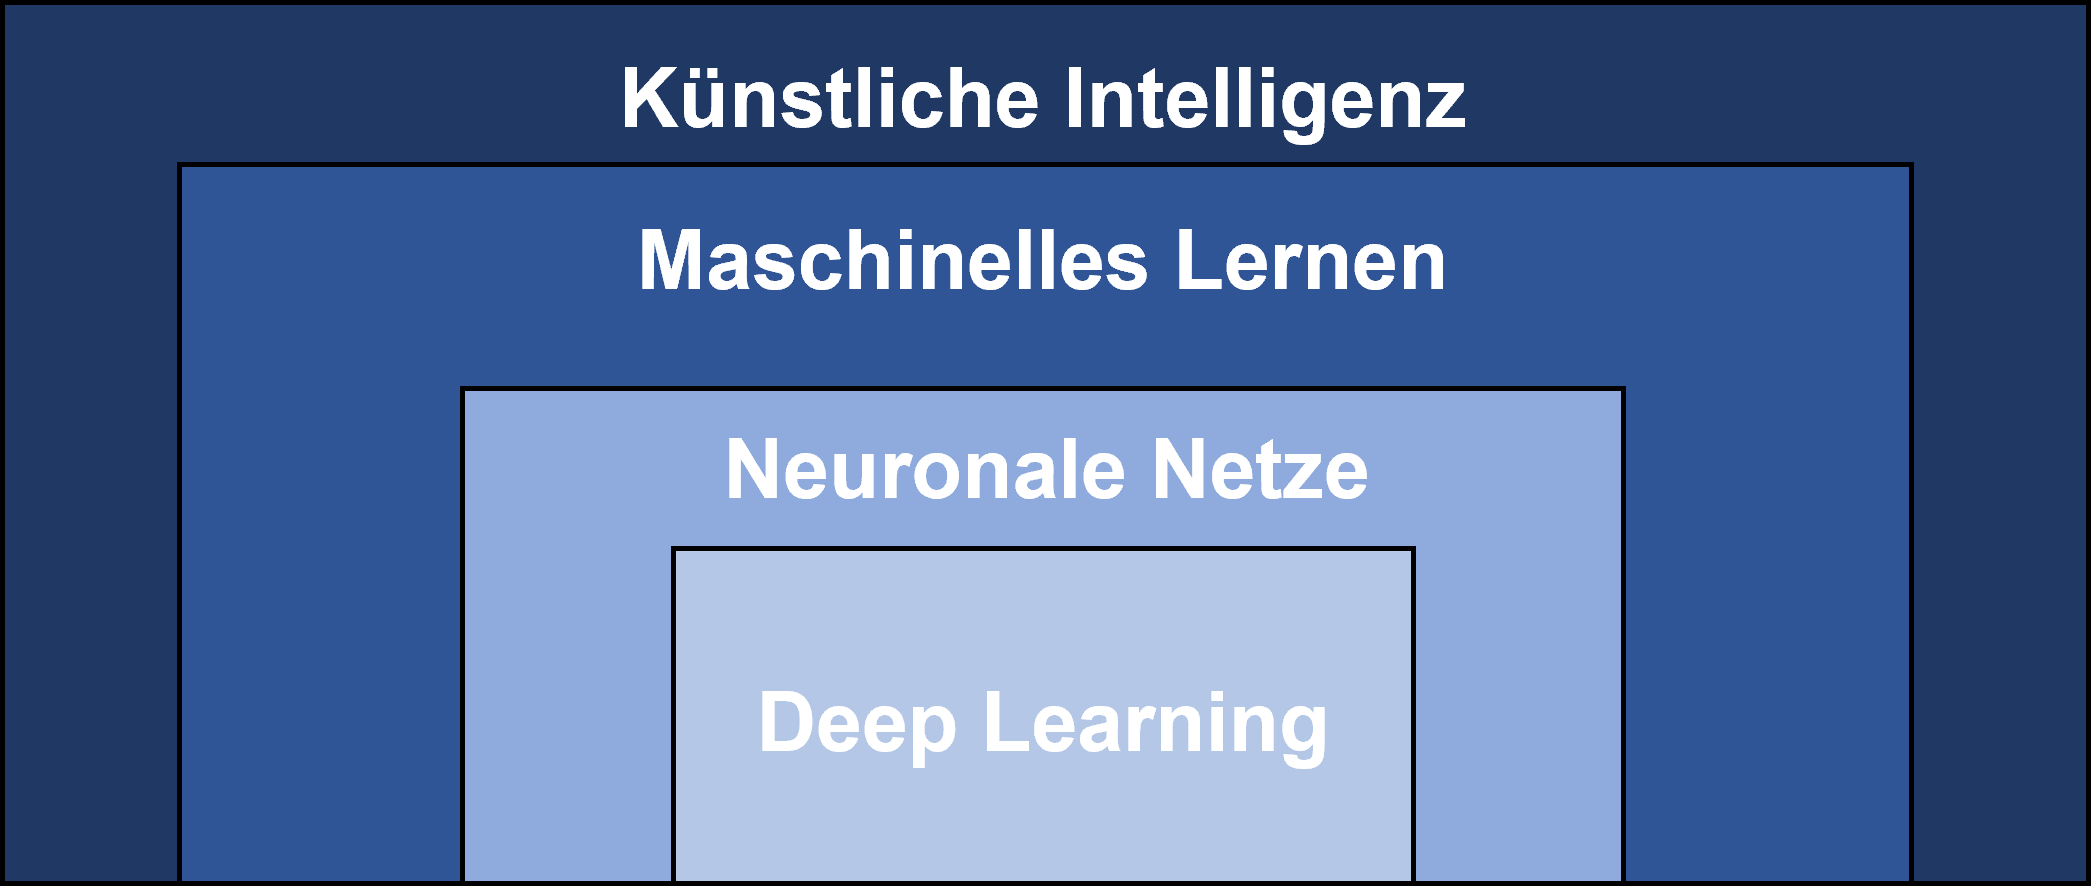
\includegraphics[scale=0.52]{pic/MA-Bilder/KI-ML-DL.PNG}
    \caption{Feld des MLs, eigene Darstellung in Anlehnung an \cite{shinde}}
    \label{Fig:KI-ML-DL}
\end{wrapfigure}
Im Zusammenhang mit dem Begriff des \glqq Maschinellen Lernens\grqq{} tauchen häufig auch Konzepte wie \glqq Künstliche Intelligenz\grqq{} (engl. Artifical Intelligence, Abk.: KI/AI), \glqq Neuronale Netze\grqq{} oder \glqq Deep Learning\grqq{} (DL) auf. Überdies werden diese Begriffe teilweise synonym verwendet, was jedoch nicht korrekt ist, obgleich eine gewisse Verwandtschaft besteht \cite{Kerner2020, shinde}. Um in Bezug auf die vorliegende Masterarbeit Klarheit zu schaffen, startet dieses Kapitel mit einer Abgrenzung dieser verschiedenen Begrifflichkeiten. Der Zusammenhang ist grob in Abbildung \ref{Fig:KI-ML-DL} dargestellt.

KI lässt sich definieren als die Befähigung \enquote{einer Maschine, menschliche Fähigkeiten wie logisches Denken, Lernen, Planen und Kreativität zu imitieren} \cite{euki}. Das ML dagegen ist ein Teilgebiet der KI und hat den automatisierten Lernprozess von Maschinen zum Gegenstand \cite{Kerner2020}.  Mithilfe von ML ist es möglich, große Datenmengen zu verarbeiten und aus diesen Entscheidungen oder Erkenntnisse abzuleiten. Abstrakter formuliert, kann ML als Berechnungsprozess verstanden werden, welcher Eingabedaten verwendet, ohne dass durch Programmcode exakt vorgegeben ist, wie schlussendlich das Ergebnis gebildet wird \cite{ElNaqa.2015b}. Neuronale Netze bilden wiederum ein Teilgebiet von ML \cite{Kerner2020}. Künstliche neuronale Netze bilden computerbasiert die Gehirnstrukturen von Menschen und Tieren nach, indem einzelne Knoten über Kanten verknüpft werden \cite{rojas2001kunstliche}. Neben den neuronalen Netzen existiert noch der Begriff des DLs. Deep Learning-Modelle sind neuronale Netze mit tieferen Strukturen, jedoch ist umstritten wie viele Schichten ein künstliches neuronales Netz zu einem \enquote{Deep Neuronal Network} (DNN) machen, und wie somit eine präzise Abgrenzung der Begriffe möglich ist \cite{Kerner2020}.

Die folgende Masterarbeit konzertiert sich auf das Forschungsfeld des MLs. Während der Literaturrecherche werden aber auch Quellen, welche KI, neuronalen Netzen oder Deep Learning zum Gegenstand haben, nicht ausgeschlossen, da diese wie gezeigt mit ML eng vermascht sind.
\subsection{Ablauf des maschinellen Lernens}
\label{subsec_AblaufML}
\begin{wrapfigure}{r}{0.5\textwidth}
    \centering
    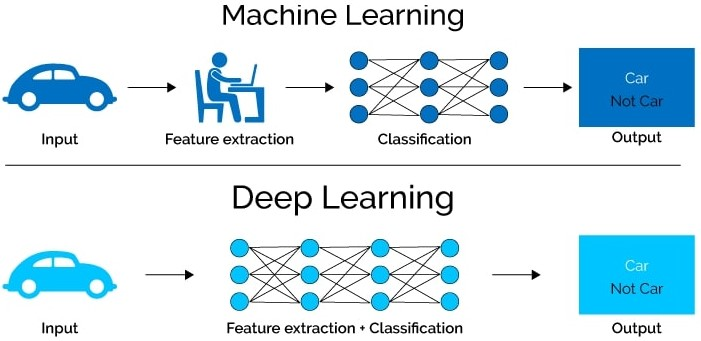
\includegraphics[scale=0.45]{pic/MA-Bilder/MLPipeline.jpeg}
    \caption{Prozess des MLs/DLs, entnommen aus \cite{WolfewiczML}}
    \label{Fig:mlpipeline}
\end{wrapfigure}
Der Ablauf beim ML kann auf unterschiedlichen Abstraktionsebenen beschrieben werden. Auf hohger Abstraktionsebene lässt sich der technische Ablauf vereinfacht in Abbildung \ref{Fig:mlpipeline} darstellen. Im Kontext dieser Masterarbeit wird der technische Ablauf des MLs von hier an als \emph{Datenfluss} bezeichnet. Ausgangspunkt für diesen Datenfluss sind Beispieldaten, welche die Grundlage für einen Algorithmus bieten, Muster und Zusammenhänge zu erkennen. Bei diesen Beispieldaten wird auch von Trainingsdaten gesprochen \cite{janiesch2021machine}. Um diese Daten für den Algorithmus effizient nutzbar zu machen, beginnt der Datenfluss mit der \emph{Feature Extraction}. Hier werden relevante Merkmale aus den Daten ausgewählt, zusammengefasst oder in ein Format überführt, welches für Maschinen leichter zu interpretieren ist \cite{janiesch2021machine}. Ein Beispiel für Feature Extraction ist im Umfeld der Textklassifikation die TF-IDF-Methode \cite{dalal2011automatic}. TF-IDF steht für \emph{term frequency-inverse document frequency} und diese gibt an, wie wichtig ein Wort in einem Text ist. Hier wird für ein Wort ein numerischer Wert zurückgegeben, mit dem ein Algorithmus besser umgehen kann. Je häufiger ein Wort vorkommt, desto höher ist der TF-IDF-Wert, wobei dieser Wert durch das Betrachten anderer Texte in einem gesamten Korpus gesenkt werden kann, um zu vermeiden, dass Wörter, welche grundsätzlich oft vorkommen, eine fälschlicherweise hohe Wichtigkeit zugesprochen bekommen \cite{bafna2016document}. Haben die Trainingsdaten die Feature-Extraction-Phase des Datenflusses passiert, beginnt der Prozess des "Model Buildings", welcher auch Training genannt wird \cite{Cady.2017, bacstanlar2014introduction}. Ergebnis des Trainings ist ein Modell, welches Zusammenhänge innerhalb der Trainingsdaten beschreibt. Das erstelle Modell kann z.B. ein Entscheidungsbaum oder ein neuronales Netzwerk sein (vgl. Kapitel \ref{subsubsec_Verfahren} \cite{Cleve.2020}. Schlussendlich soll das erstellte Modell den zweck erfüllen, Vorhersagen zu treffen, wie z.B. das Klassifizieren von unbekannten Datensätzen \cite{Wuttke.2022}. 

Neben dem eher technisch orientierten Datenfluss, können prozessual allerdings noch weitere organisatorische und inhaltliche Aspekte in den Vordergrund rücken. Grundsätzlich muss zu Beginn die Art des Problems identifiziert werden \cite{Verdhan.2020}. Weiter muss sich für einen konkreten Algorithmus (vgl. Kapitel \ref{subsubsec_Verfahren} entschieden werden \cite{ayodele}. Organisatorisch steht besonders bei ML-Projekten im Vordergrund, ob, wo und in welchem Format Trainingsdaten vorliegen. Weiter müssen diese Daten unter Umständen noch bereinigt oder auf ihre notwendigen Datenfelder herunter gebrochen werden \cite{Verdhan.2020}. Auch ist es möglich, dass Datensätze künstlich expandiert werden, was beispielsweise in der Bilderkennung häufig vorkommt. Hier werden Bilder aus den Trainingsdaten rotiert oder gespiegelt, um mehr Trainingsdaten für den Algorithmus zu generieren um somit z.B. Überanpassung zu vermeiden \cite{mikolajczyk2018data}. Nach der Feature Extraction und dem Training muss sich auch noch über die Auslieferung des Modells in den produktiven Betrieb Gedanken gemacht werden \cite{Verdhan.2020}. Weiter kann während des Betriebs auch das sog "Liefelong Learning" berücksichtigt werden. Dieses Lernparadigma zählt darauf ab, dass ein Algorithmus neues lernt, während er dabei auf bestehenden Wissen aufbaut \cite{chen2018lifelong}.
\todo[inline]{Ein Kapitel zu Über- und Unteranpassung und Bias?}

Bei der Herausforderung inhaltliche und organisatorische Ebenen von ML-Projekten zu überblicken helfen in der Praxis Vorgehensmodelle. Bekannte Beispiele hierfür sind der \emph{Cross-Industry Standard Process for Data-Mining} (CRISP-DM) und der \emph{Knowledge Discovery in Databases}-Prozess (KDD) \cite{weber2019new}. Das Prozessmodell CRISP-DM wurde von dem amerikanischen IT-Unternehmen \emph{IBM} entwickelt. CRISP-DM bezieht in mehreren Phasen unter anderem das Schaffen von Verständnis für die Domäne und die Daten mit ein. Ferner legt es Vorgaben für die Datenvorbereitung, Modellierung und Evaluation des Modells fest. Daneben wird auch der produktive Einsatz des generierten ML-Modells mit betrachtet \cite{IBMCRISP}. Das KDD-Prozess kann auch Anwendung bei ML-Projekten finden, setzt hierbei allerdings einen eher technischen Fokus \cite{weber2019new, fayyad1996data}. Dieses Modell legt in den ersten vier Phasen den Fokus auf die Datenauswahl, -vorbereitung, -transformation und Mustererkennung. Die letzte Phase beinhaltet die Interpretation und das Schaffen von Wissen \cite{fayyad1996data}. Weber et al. \cite{weber2019new} merken jedoch an, dass diese Modelle trotz ihres vielfachen Einsatzes in der Praxis auch Schwächen aufweisen. Dies begründen die Autoren damit, dass die experimentelle und die operative Phase des MLs nicht genügend Aufmerksamkeit bekommt \cite{weber2019new}. Geschlossen wird diese Lücke vom Konzept des \emph{Machine Learning Operations} (MLOps). Kreuzberger et al. \cite{kreuzberger2022machine} stellen heraus, welche Prozesse und Prinzipien dabei helfen ML-Projekte ganzheitlich bis hin zum Betrieb zu betrachten. Hierbei werden neben technischen Kompontenten oder Rollen, wie z.B. die eines Software Engineers auch prozessuale Elemente wie Automatisierung mitbedacht \cite{kreuzberger2022machine}.
\subsection{Typen des maschinellen Lernens}
\label{chap:Types}
Einzelne Algorithmen des MLs lassen sich zumeist einer von mehreren Klassen zuordnen. Hauptunterscheidungsmerkmal dieser Kategorien besteht in der Art des Lernens sowie in der Beschaffenheit der Ein- und Ausgabedaten. Die drei am häufigsten genannten Klassen sind überwachtes Lernen (engl.: \emph{supervised learning}), unüberwachtes Lernen (engl.: \emph{unsupervised learning}) und bestärkendes Lernen (engl.: \emph{reinforcement learning}), wobei auch noch Mischformen wie teilüberwachtes Lernen (engl.: \emph{semi-supervised learning}) existieren \cite{Alpaydin+2019, Wuttke.2022, ayodele}.

\textbf{Überwachtes Lernen}
\begin{addmargin}[25pt]{0pt}
Überwachtes Lernen ist der am häufigsten genutzte Typ des maschinellen Lernens. Hierbei lernt ein Computerprogramm, indem es sich bestehende Daten zu Nutze macht \cite{Verdhan.2020}. Diese zu Beginn vorhandenen Datensätze enthalten immer einen Input und einen Output \cite{Alpaydin+2019, Choo.2020}. Ein Algorithmus soll lernen, wie Merkmale, welche sich in den Daten befinden, mit den Zielvariablen zusammenhängen \cite{Wuttke.2022}. Es soll also eine Funktion $f:x \rightarrow y$ entstehen, welche folgende Input-Paare $\{(x\textsubscript{1}, y\textsubscript{1}), ... , (x\textsubscript{i}, y\textsubscript{i})\}$  aufeinander abbildet. Schlussendlich sollen Zielvariablen ($y$-Werte) für neue, unbekannte $x$-Werte mit der Funktion vorhergesagt werden \cite{Choo.2020}.

Typisch für Probleme, welche mithilfe von überwachtem Lernen angegangen werden, sind Klassifikations- und Regressionsprobleme\todo{Später überdenken: eigenes Kapitel für Anwendungsfälle sinnvoll?}. Klassifikationsalgorithmen beispielweise ermöglichen es auf Bildern zu erkennen, ob es sich um eine Katze oder einen Hund handelt. Die im vorherigen Abschnitt angesprochene Zielvariable y wäre in diesem Fall ein Wert, welcher einer Kategorie, also Hund oder Katze, entspräche. Ein Beispiel für ein Regressionsproblem ist die Vorhersage von Regentagen auf Grundlage historischer Niderschlagsmengen \cite{Choo.2020}. 
\end{addmargin}

\textbf{Unüberwachtes Lernen}
\begin{addmargin}[25pt]{0pt}
Im Gegensatz zum überwachten Lernen stehen beim unüberwachtem Lernen keine Trainingsdaten mit Zielvariablen zur Verfügung \cite{ayodele}. Das Ziel bleibt jedoch, dass eine Funktion erstellt werden soll, die Eingabe- auf Ausgabewerte $f:x \rightarrow y$ abbildet, jedoch ohne Kenntnisse über $y$ \cite{Alpaydin+2019}. Algorithmen des unüberwachten Lernens funktionieren so, dass sie den Daten Informationen extrahieren und folglich Muster in den Daten entdecken \cite{Choo.2020, Verdhan.2020}.

Beispiele für die Anwendung von unüberwachtem Lernen sind Clusteranalysen oder Assoziationsalanysen \cite{Wuttke.2022}. Bei einer Clusteranalyse werden Daten aufgrund ähnlicher Muster oder gleicher Attribute gruppiert. Muster können dadurch entstehen, dass z.B. bei Entitäten eines Clusters die gleichen Merkmale vorhanden sind oder fehlen. Als praxisnaher Anwendungsfall sei hier die Kundensegmentierung genannt, welche es einem Unternehmen ermöglicht verschiedene Marketingstrategien passend für unterschiedliche Kundensegemente zu entwickeln. Merkmale, die im Rahmen einer Clusteranalyse ins Gewicht fallen, wären z.B. das Alter, der Umsatz oder das Online/Offline-Verhalten \cite{Verdhan.2020}.
Assoziationsanalyse als weiteres Beispiel des unüberwachten Lernens haben zum Gegenstand Assoziationsregeln zu finden, die Zusammenhänge zwischen verschiedenen Attributen darstellen, wie es z.B. in der Warenkorbanalyse der Fall ist. Hier wird versucht, anhand von bestimmten im Warenkorb befindlichen Produkten auf andere Produkte zu schließen \cite{Cleve.2020}. Eine Regel, welche ein Algorithmus der Assoziatitonsanalyse aufstellen würde, könnte beispielsweise lauten: \textit{Wer Müsli kauft, der kauft auch Milch}.
\end{addmargin}

\textbf{Teilüberwachtes Lernen}
\begin{addmargin}[25pt]{0pt}
Das teilüberwachte Lernen bildet die Mischform des über- und unüberwachten Lernens, denn hier werden sowohl Daten mit Zielvariablen als auch Daten ohne Zielvariablen zum Trainieren des Algorithmus verwendet \cite{ayodele}. Teilüberwachtes Lernen ist meistens dann sinnvoll, wenn einige Daten mit Zielvariable, jedoch gleichzeitig auch viele ohne Zielvariable vorhanden sind und es sehr teuer oder aufwendig wäre, die fehlenden Zielvariablen zu erheben \cite{Wuttke.2022}. Die Grundidee des teilüberwachten Lernens ist, dass Daten, welche sich im gleichen Cluster befinden, wahrscheinlich auch zur gleichen Klasse gehören. Diese Erkenntnis kann genutzt werden, um eine bessere Datenbasis zu generieren. Somit können beide ML-Ansätze kombiniert werden \cite{Verdhan.2020}.
\end{addmargin}

\textbf{Bestärkendes Lernen}
\begin{addmargin}[25pt]{0pt}
Das bestärkende Lernen beschäftigt sich damit, wie mehrere Aktionen aufeinander folgen sollen. Ein Algorithmus lernt basierend auf Belohnungen oder Bestrafungen, welche durch seine Umwelt signalisiert werden, wie er zu handeln hat \cite{Lorenz.2020}. Dieses Feedback ist zwingend erforderlich, um selbstständig lernen zu können \cite{Wuttke.2022}. Ziel ist es mit  zukünftigen Aktionsreihenfolgen die Belohnungen zu maximieren \cite{Lorenz.2020}. Weiter ist nicht eine einzige Aktionen, sondern mehrere aufeinander folgende Aktionen zusammengefasst als Taktik, entscheidend für die angemessene Funktionsweise des Algorithmus \cite{Alpaydin+2019}. 

Ein prominentes Beispiel für bestärkendes Lernen ist die von Google entwickelte Software \textit{AlphaGO}, welche mittels Datensammlungen über von Menschen gespielter Partien, geeignete Taktiken entwickeln konnte, um gegen den erfolgreichsten menschlichen Spieler im  Brettspiel GO gewinnen zu können \cite{Wuttke.2022}.
\end{addmargin}

Je nach dem, welcher Typ zur Anwendung kommt, entstehen Differenzen bzgl. des technischen Ablauf des MLs, welcher im vorherigen Kapitel \ref{subsec_AblaufML} dargestellt wurde. Beim überwachten Lernen wird dem Lernprozess die Teilung der Beispieldaten vorangestellt. Der Datensatz wird hier in einen Trainings- und ein Testdatensatz aufgeteilt. Diese Testdaten werden genutzt, um das erstellte Modell auf seine Funktionsweise und inhaltliche Zuverlässigkeit zu testen \cite{kotsiantis2007supervised}. Es ist für die Funktionsweise des Algorithmus und die Performance während des Trainings jedoch nicht unerheblich, wie groß diese Datensätze im Verhältnis sind \cite{nguyen2021influence}. Auch beim bestärkenden Lernen kommen Testdaten zum Einsatz \cite{Lorenz.2020}. Da die Trainingsdaten, welche beim unüberwachten Lernen vorliegen, über keine Zielvariablen verfügen, kann die Überprüfung des erzeugten Modells nicht wie beim überwachten Lernen mithilfe von Testdaten erfolgen \cite{ayodele}. Alternativen, um das Modell bei diesen Algorithmen zu überprüfen, bestehen beispielsweise in Metriken, welche überprüfen, wie kompakt die verschiedenen Cluster erstellt wurden, oder in Kreuzvalidierung \cite{halkidi2001clustering, perry2009cross}.  

An dieser Stelle sei angemerkt, dass neben der Funktionweise auch andere Qualitätsmerkmal bei ML eine Rolle spielen können. So kann die Performance oder Nutzung des Hardwarespeichers auch entscheidend bei der Implementierung eines ML-Algorithmus sein \cite{coleman2019analysis}. Daneben existieren noch weitere Methoden zur Evaluation im ML, welche es z.B. ermöglichen, verschiedene Instanzen des gleichen Algorithmus oder auch unterschiedliche Algorithmen untereinander zu vergleichen \cite{raschka2018model}.
\subsection{Verfahren des maschinellen Lernens}
\label{subsubsec_Verfahren}
Es existieren viele konkrete Algorithmen des MLs, welche sich in eine oder mehrere der vorher genannten Typen einordnen lassen. Folgend werden die theoretischen Grundlagen der jeweiligen Algorithmen erläutert. Die in der Literatur und Praxis häufig genannten ML-Verfahren sind: Entscheidungsbäume, logistische Regression, Bayessche Modelle, Support Vector Machines, k-means Clustering, k-nearest Neighbours sowie neuronale Netze \cite{alzubi2018machine, MicrosoftML, dobel2018maschinelles, sarker2021machine}. \todo[noline]{Diese Auswahl am Ende noch einmal überdenken/anpassen} Um den Umfang nicht zu sprengen, wird sich auf diese häufig genannten konzentriert.
%Fraunhofer Quelle hat sogar eine Befragung gemacht

\subsubsection{Entscheidungsbäume}
\label{chap_dectree}
\begin{wrapfigure}{r}{0.5\textwidth}
    \centering
    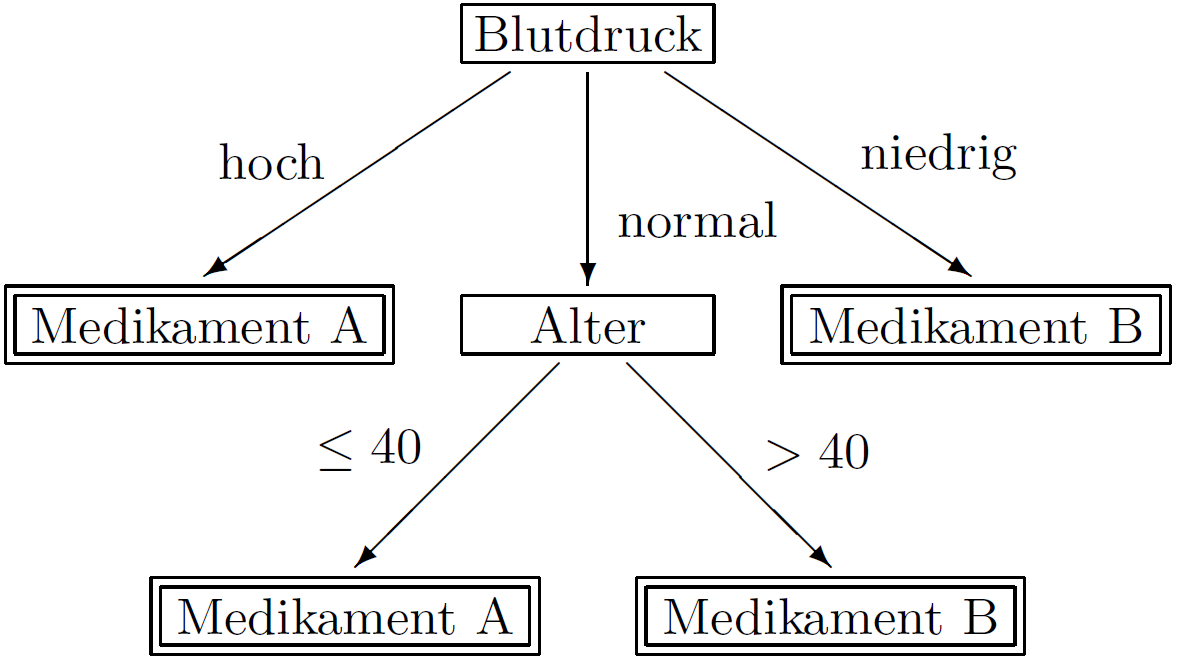
\includegraphics[scale=0.33]{pic/MA-Bilder/Entscheidungsbaum.PNG}
    \caption{Beispiel für einen Entscheidungsbaum \cite{borgelt1998attributauswahlmasse}}
    \label{Fig:dectree}
\end{wrapfigure}
Entscheidungsbäume können zur Klassifikation oder Regression eingesetzt werden \cite{Wuttke.2022}. Entscheidungsbäume, welche zur Klassifikation eingesetzt werden, teilen eine Menge immer wieder in unterschiedliche Teilmengen auf. Die letzte Unterteilung entspricht der Klasse zu der eine Entität gehört \cite{Breiman.2017}. Bei dieser schrittweisen Aufteilung spricht man auch von rekursiver Partitionierung \cite{Ng.2018}. Soll ein Entscheidungsbaum konstruiert werden, kann wie folgt vorgegangen werden: man starte zunächst mit der Wurzel, die ein erstes Entscheidungskriterium beinhaltet. Von dieser Wurzel aus können mehrere Kanten ausgehen, welche zu anderen Knoten führen. An diesen Knoten können sich wiederum Entscheidungskriterien mit neuen Kanten befinden. Knoten ohne Nachfolger bilden die Blätter und somit auch die Kategorien des zugrundeliegenden Klassifikationsproblems \cite{Wuttke.2022}. Ein Beispiel für einen Entscheidungsbaum ist in Abbildung \ref{Fig:dectree} zu sehen.

Entscheidungsbäume haben jedoch einige Nachteile, so können geringe Änderungen im Trainingsdatensatz große Auswirkungen im Design des Baumes nach sich ziehen. Überdies können unglücklich ausgewählte binäre Entscheidungskriterien am Baumknoten ungenaue Endergebnisse hervorrufen. Abhilfe kann eine mögliche Abwandlung von Entscheidungsbäumen schaffen, welche die Komplexität des Algorithmus jedoch erhöht. Dieses Verfahren heißt \enquote{Random Forest}, da dort verschiedene, zufällig erzeugte Entscheidungsbäume zur gleichen Zeit arbeiten. Am Ende werden über die Ergebnisse aller Bäume ein Mittelwert gebildet oder auf andere Weise zu einer endgültigen Antwort zusammengefasst \cite{Ng.2018}.

\subsubsection{k-means Clustering}
\label{subsubsec:k-means-Clustering}
\begin{wrapfigure}{r}{0.5\textwidth}
    \centering
    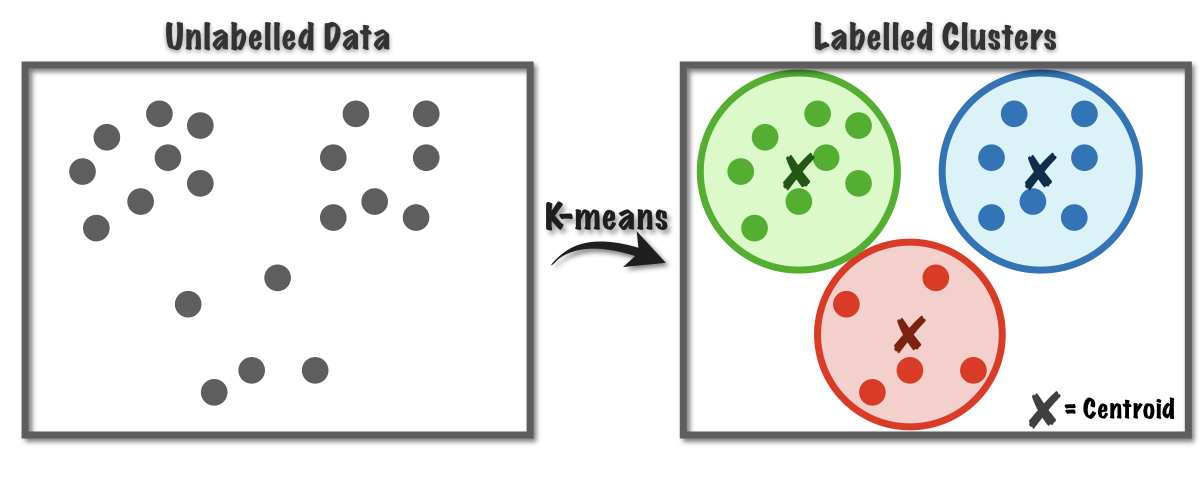
\includegraphics[scale=0.16]{pic/MA-Bilder/k-means-Clustering.png}
    \caption{Input und Output des \emph{k-means Clustering}-Verfahrens, entnommen aus \cite{Fiori-online}}
    \label{Fig:kmeans}
\end{wrapfigure}
Das \emph{k-means Clustering}-Verfahren ist ein Algorithmus des unüberwachten Lernens und kann bspw. dazu eingesetzt werden gezielte Werbestrategien zu entwickeln \cite{Matzka.2021, Ng.2018}. So können Kunden, die bestimmte Merkmale, z.B. Einkommen oder Persönlichkeitszüge wie Offenheit gemeinsam haben, die gleichen Produkte vorgeschlagen werden \cite{Ng.2018}. Das \emph{k-means Clustering}-Verfahren unterstützt dies, indem es Kunden (oder universell formuliert Datenpunkte) einem von $k$ Clustern zuordnet \cite{ayodele}. $k$ muss bei diesem Verfahren vorgegeben werden. Im Fokus des Verfahrens steht die Ermittlung der Zentren (engl.: \emph{Centroide}) eines jeden Clusters \cite{Cleve.2020}.
\newline

Die Funktionsweise des Verfahrens lässt sich in etwa wie folgt umreißen: zu Beginn werden (zufällig) die Standorte der $k$ Zentren gewählt \cite{Cleve.2020}. Als nächstes wird für jeden Datenpunkt das ihm am nächsten liegende Zentrum gefunden. Ist dies für jeden Datenpunkt erfolgt, werden neue Zentren ermittelt, indem die Mittelpunkte aller einem Zentrum zugehörigen Datenpunkte berechnet werden. Als nächstes folgt eine erneute Zuordnung aller Datenpunkte zu den neuen Zentren. Diese Zuordnung und Zentrenbildung wird so lange wiederholt bis sich keine neuen Zentren mehr auffinden lassen \cite{Ng.2018}. Abbildung \ref{Fig:kmeans} visualisiert das Endergebnis des \emph{k-means Clustering}-Verfahrens beispielhaft.

 \emph{k-means Clustering} ist aufgrund seiner geringen Komplexität während der Implementierung beliebt. Vereinfacht gesagt, müssten bei einer Realisierung des Algorithmus nur immer wieder neue Abstände berechnet werden und draufhin die Datenpunkten (erneut) den Clusterzentren zugeordnet werden \cite{Cleve.2020}. Neben dieser Einfachheit existieren jedoch auch einige Schwächen, wie z.B. die Form der Cluster. Durch die iterative Anwendung entstehen kreisförmige Cluster. In der Realität ist es jedoch nicht selten, dass die realen Cluster ein anderes, z.B. elliptisches Erscheinungsbild besitzen \cite{Ng.2018}.  Weiter ist der Algorithmus anfällig in Bezug auf Rauschen und Ausreißer \cite{Cleve.2020}. Als Ausreißer bezeichnet man Datenpunkte, welche sich von den anderen stark unterscheiden. Ein Beispiel hierfür könnten Kundendaten sein, welche das Alter der Personen beinhalten. Wären alle Kunden 20-30 Jahre alt, aber gäbe es einen Kunden, welcher 80 Jahre als ist, wäre dies der Ausreißer \cite{Cleve.2020}. Rauschen in Daten kann sich in Form verschiedenster Anomalien bemerkbar machen. Beispielsweise kann es zu Messfehlern bei der Datenbeschaffung gekommen sein, wohingegen auch die Betrachtung zu vieler Attribute beim Lernprozess ein Rauschen verursachen kann \cite{Alpaydin+2019}. Daneben ist es nicht vorgesehen, dass sich Cluster gegenseitig überlappen \cite{Ng.2018}. Weiter sei angemerkt, dass die Ermittlung von $k$, also die Anzahl der Cluster, nicht durch das Verfahren gelöst wird und diese Entscheidung durch den Anwender getroffen werden muss \cite{Cleve.2020}.
 
 \subsubsection{Support Vector Machines}
 \begin{wrapfigure}{r}{0.5\textwidth}
    \centering
    \raisebox{0pt}[\dimexpr\height-0.7\baselineskip\relax]{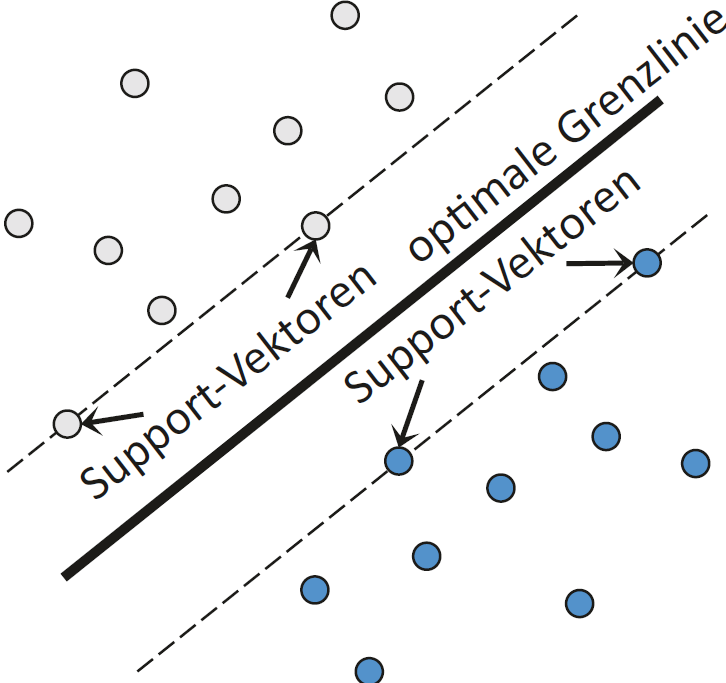
\includegraphics[scale=0.3]{pic/MA-Bilder/support-vector-machines.PNG}}
    \caption{SVM \cite{Ng.2018}}
    \label{Fig:svm}
\end{wrapfigure} 
\emph{Support Vector Machines} (SVM) können zur Klassifikation eingesetzt werden und gehören zu den Algorithmen des überwachten Lernens \cite{Verdhan.2020}. Ziel des Algorithmus ist die Ermittlung einer Grenzlinie (engl.: \emph{Hyperplane}), welche die Datenpunkte zweier oder mehrerer Klassen separiert \cite{Ng.2018, noble2006support}. Im zwei-dimensionalen Raum kann man sich die Separierung der Daten als Gerade vorstellen \cite{Verdhan.2020}. Zur Ermittlung der Grenzlinie ist es erforderlich \enquote{diejenigen Datenpunkte am Rand ihrer jeweiligen Gruppe zu finden, die am nächsten zu den Punkten der jeweils anderen Gruppe gelegen sind} \cite{Ng.2018}. Diese Randpunkte werden als \emph{Support-Vektoren} bezeichnet. Werden die Randpunkte der jeweiligen Klassen verbunden, entstehen zwei Linien. In der Mitte dieser zwei Linien, liegt nun die Hyperplane, was in Abbildung \ref{Fig:svm} visualisiert ist \cite{Ng.2018}. Der SVM-Algorithmus hat folglich zur Aufgabe die Abstände zwischen den \emph{Support-Vektoren} zu maximieren, um die optimale Grenzlinie zu ermitteln, welche die Klassifikation unbekannter Datensätze ermöglicht \cite{Matzka.2021}.

SVM zeichnet ihre Flexibilität in der Separierung aus. Während in Kapitel \ref{chap_dectree} angemerkt wurde, dass das \emph{k-means Clustering}-Verfahren die gefundenen Cluster nur kreisförmig darstellen kann, ermöglicht es die \emph{Kernel}-Taktik hingegen mit SVM auch andere Formen darzustellen. Hierbei kommt es zu einer leichten Abwandlung des Verfahrens, sodass der Algorithmus in höheren Dimensionen angewendet wird und somit z.B. elliptische Abgrenzungen anstatt Geraden ermöglicht werden \cite{Ng.2018}. Weiter können auch Klassifikationen im $n$-dimensionalen Raum mithilfe einer Ebene, welche die Dimension $n-1$ besitzt, realisiert werden \cite{Cleve.2020}. Ein weiterer Vorteil der SVM besteht in der Rigorosität gegenüber Ausreißern durch bestimmte Anpassungen des Verfahrens. So besteht die Möglichkeit Daten, die sowohl nah an der einen als auch an der anderen Gruppe liegen, lediglich mit gewissen Wahrscheinlichkeit einer Gruppe zuzuordnen. Diese Wahrscheinlichkeiten lassen sich durch die Betrachtung des Abstandes zur Grenzlinie berechnen \cite{Ng.2018}.

\subsubsection{Logistische Regression}
\begin{wrapfigure}{r}{0.4\textwidth}
    \centering
    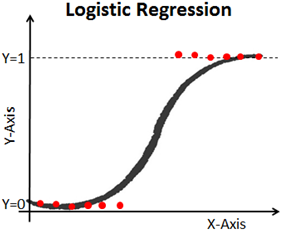
\includegraphics[scale=0.9]{pic/MA-Bilder/logistische-Regression.png}
    \caption{Logistische Regression \cite{Ng.2018}}
    \label{Fig:logistic regression}
\end{wrapfigure}
Die logistische Regression verfolgt das Ziel die Wahrscheinlichkeit des Auftretens einer binären Zielgröße vorherzusagen. Diese Vorhersage kann abhängig von bestimmten Merkmalen getroffen werden. Ein beispielhaftes Szenario, mit dem sich logistische Regression beschäftigen könnte, besteht darin auf Grundlage von Geschlecht und Blutwerten vorherzusagen, wie wahrscheinlich es ist, dass eine Person erkrankt oder nicht erkrankt \cite{Kalisch.2021}. Anders als der Name des Verfahrens logistische \enquote{Regression} vermuten lässt, geht es hier weniger um Regression, sondern eher um Klassifikation \cite{Kersting.2019}. Zur Vorhersage der Wahrscheinlichkeiten wird eine logistische Funktion erstellt. Anders als es in der linearen Regression, in der versucht wird konkrete Werte mithilfe einer Geraden darzustellen, gefordert, ermöglicht es die logistische Funktion Wahrscheinlichkeiten abzubilden \cite{Behnke.2015}. Durch ihr s-förmiges Erscheinungsbild ist diese Funktion in der Lage \enquote{reelwertige Variablen} $[+\infty, -\infty]$ in den Wertebereich von 0 bis 1 zu transformieren \cite{Backhaus.2016}. Die entsprechenden Funktionsparameter der gewünschten logistischen Zielfunktion lassen sich mit der sogenannten \emph{Maximum-Likelihood}-Methode finden \cite{Backhaus.2016}. Diese Methode nähert sich iterativ den Parametern an und sucht diejenige Konstellation der Funktionsparameter, bei der es am wahrscheinlichsten ist, dass die im Trainingsdatensatz vorhandenen Beobachtungen auftreten \cite{Behnke.2015}.

\subsubsection{k-Nächste Nachbarn}
\label{subsubsec_KNN}
\begin{wrapfigure}{R}{0.4\textwidth}
    \centering
    \raisebox{0pt}[\dimexpr\height-1.5\baselineskip\relax]{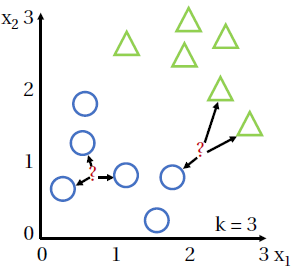
\includegraphics[scale=0.7]{pic/MA-Bilder/k-naechste-Nachbarn.PNG}}
    \caption{Beispiel für kNN mit k=3 \cite{Matzka.2021}}
    \label{Fig:knearest}
\end{wrapfigure}
Das \emph{k-nächste Nachbarn}-Verfahren (kNN) als ML-Algorithmus des überwachten Lernens kann zur Lösung von Klassifikationsproblemen herangezogen werden. Bei der Zuordnung unbekannter Entitäten zu einer Klasse macht kNN sich bestehende Ähnlichkeiten zu bereits zugeordneten Entitäten zu Nutze \cite{Matzka.2021}. Ein herausstellendes Merkmal dieses Verfahrens besteht darin, etwas von dem in Kapitel \ref{subsec_AblaufML} beschrieben Datenfluss abgewichen wird. Bei diesem Algorithmus wird in der Trainingsphase kein Modell erstellt, welches später Zuordnungen vornehmen kann, sondern die Berechnungen und die Klassifikation einzelner Datensätze finden zum selben Zeitpunkt statt \cite{Verdhan.2020, Matzka.2021}. Bei der Bestimmung der Klassenzugehörigkeit, prüft das kNN-Verfahren, wie weit dieser von anderen bereits klassifizierten Datensätzen entfernt ist \cite{Verdhan.2020}. Der Parameter $k$ in kNN steht für die Anzahl der Nachbarn, welche betrachtet werden sollen. Wird $k=1$ gewählt, bestimmt lediglich der nächste Nachbar das Klassenlabel. Wird sich bei der Implementierung für $k=n$ entschieden, fließen die n nächsten Nachbarn in die Entscheidungsbildung mit ein \cite{Matzka.2021}. In Abbildung \ref{Fig:knearest} ist die Funktionsweise des Verfahrens für $k=3$ beispielhaft abgebildet. An dieser Stelle sei angemerkt, dass die Bestimmung von $k$ wichtig für eine angemessene Funktionsweise des Verfahrens ist. Wird k ein kleiner Wert zugewiesen, wird sich bei der Klassenbildung nur auf wenige Daten gestützt, was besonders häufig zu Fehlklassifikation führen kann. Haben jedoch zu viele nächste Nachbarn an der Entscheidungsfindung ihren Anteil, werden Muster unter Umständen nicht präzise genug abgebildet. Neben der Festsetzung des Parameters k besteht eine wichtige Entscheidung darin, wie bei $k\geq 2$ entschieden wird, sollten Nachbarn unterschiedliche Klassenlabels besitzen. Eine Möglichkeit besteht darin, die Klassen aller k-nächsten Nachbarn in die Entscheidung miteinzubeziehen, indem der Mittelwert aller betrachteten Klassen gebildet wird. Alternativ dazu kann es jedoch auch als sinnvoll erachtet werden, solchen Nachbarn, für die eine geringere Distanz gemessen wurde, eine größere Wichtigkeit zuzusprechen \cite{Ng.2018}.

Neben seiner leichten Implementierung hat das kNN-Verfahren den Vorteil, dass es zur Erkennung von Ausreißern genutzt werden kann \cite{Ng.2018, Verdhan.2020}. Eine Schwierigkeit, welche dieses Verfahren jedoch mit sich bringt, ist die Abhängigkeit vom Wert $k$. Dieser trägt viel zu der Präzision der Vorhersagen bei, wohingegen er gleichzeitig nicht leicht zu bestimmen ist. Ferner können sich überlappende Klassen mithilfe von kNN nicht berücksichtigt werden. Dazu ist der Algorithmus langsam und rechenintensiv, da für jeden Punkt zunächst alle Abstände berechnet werden müssen und zusätzlich ein (gewichtetes) Mittel bestimmt werden muss \cite{Verdhan.2020}.

\subsubsection{Bayessche Netze}
Bayessche Netze können Prognosen für Größen, das Eintreffen bestimmter Ereignisse oder die Zugehörigkeit zu einer Klasse abgeben \cite{Dorn.2018, dehen2012bayes}. Ein bayessches Netz betrachtet Variablen und deren Abhängigkeiten zueinander, um Wahrscheinlichkeitsaussagen zu treffen. Bayessche Netze basieren auf dem Satz von Bayes \cite{dobel2018maschinelles}. Dieser Satz trifft Aussagen darüber, wie wahrscheinlich es ist, dass ein bestimmtes Ereignis eintritt, unter der Bedingung, dass ein anderes Ereignis eingetreten ist \cite{Dorn.2018}. Bayessche Netze sind gerichtete Graphen, welche diesen Satz anwenden \cite{Dorn.2018, dobel2018maschinelles}. In solchen Graphen stellen die Knoten Ereignisse oder Größen dar, während die Kanten die Abhängigkeiten der verschiedenen Knoten abbilden. Jeder Knoten besitzt mindestens zwei mögliche Zustände, wie z.B. wahr oder falsch. Darüber hinaus werden den Knoten Wahrscheinlichkeitswerte in tabellarischer Form zugewiesen. In diesen Netzen können bestimmte Arten von Beziehungen existieren. So kann ein Ereignis ein anderes bedingen. Auch möglich ist, dass mehrere vorgeschaltete Ereignisse in Kombination Auswirkungen auf ein weiteres haben \cite{dehen2012bayes}. In der Abbildung \ref{Fig:bnetz} ist ein simples bayessches Netz dargestellt. Bei bewölkten Wetter ist es sehr wahrscheinlich, dass es regnet, während es weniger wahrscheinlich ist, dass ein Rasensprenkler gestartet wird. Regen und ein Rasensprenkler in Kombination bedingen mit hoher Wahrscheinlichkeit, dass der Rasen nass wird \cite{dobel2018maschinelles}. Auf Grundlage von (kausalen) Beziehungen kann also die Wahrscheinlichkeit für das Eintreten eins bestimmten Ereignisses (Nasses Gras) berechnet werden, wenngleich die Wahrscheinlichkeit für genau dieses Ereignis - \enquote{Nasses Gras} - im Vorhinein nicht bekannt war \cite{dobel2018maschinelles, dehen2012bayes}. Die entsprechenden Werte lassen sich mithilfe des Satz von Bayes berechnen \cite{dehen2012bayes}.
\begin{figure}
    \centering
    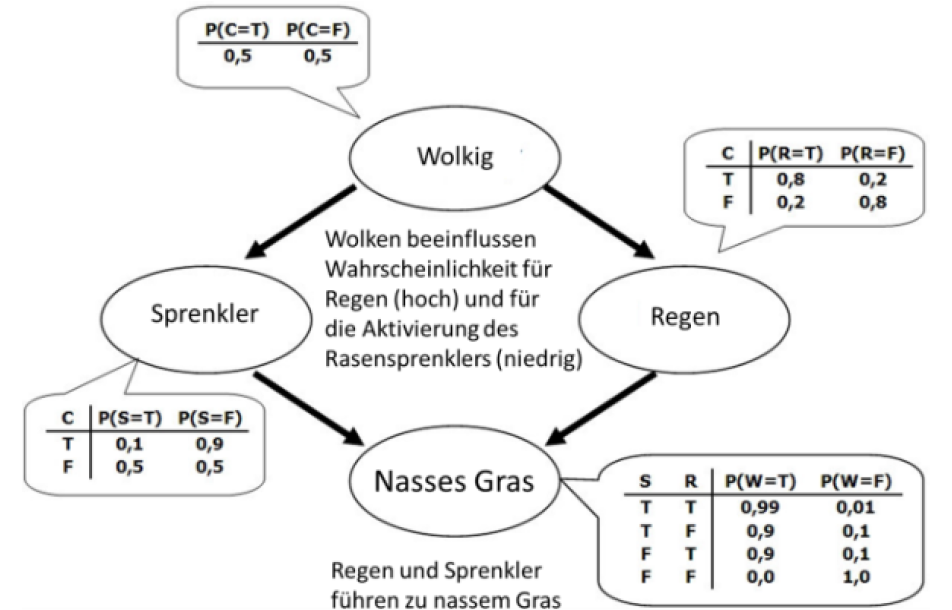
\includegraphics[scale=0.5]{pic/MA-Bilder/bayesNetz.PNG}
    \caption{Beispiel für Bayessche Netze, entnommen aus \cite{dobel2018maschinelles}}
    \label{Fig:bnetz}
\end{figure}%

\begin{wrapfigure}{r}{0.48\textwidth}
    \centering
    \raisebox{0pt}[\dimexpr\height-1.9\baselineskip\relax]{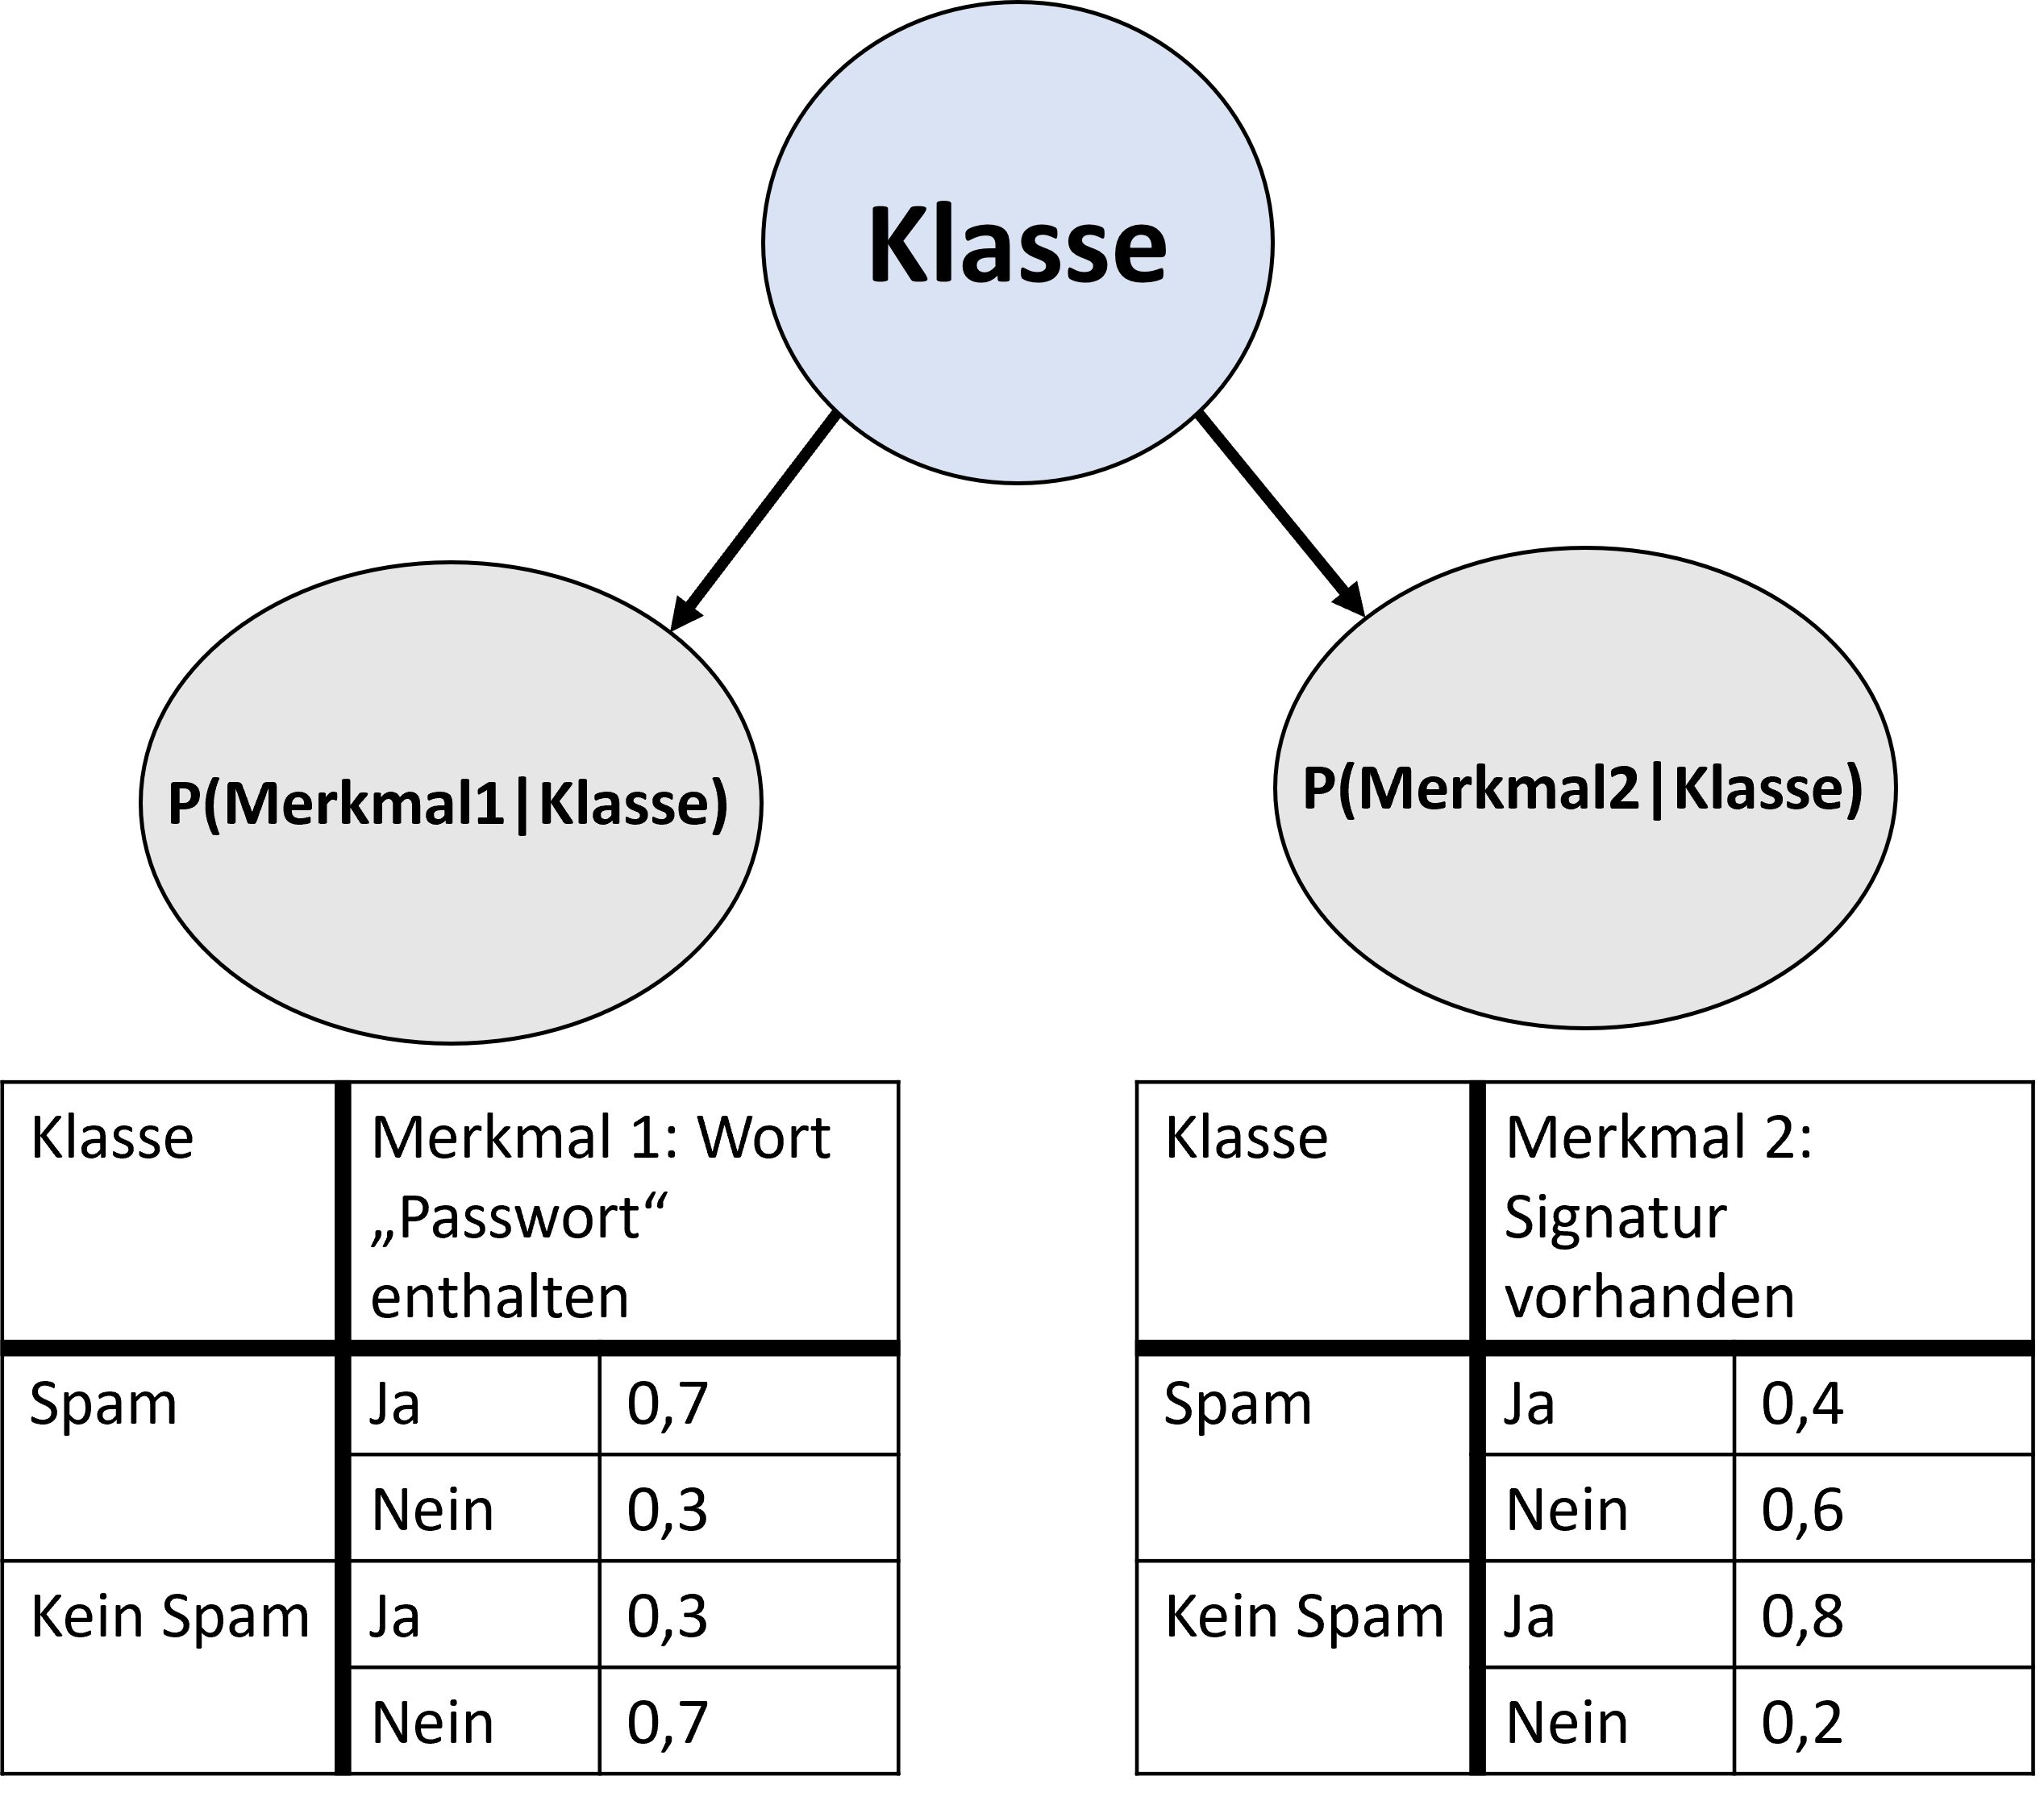
\includegraphics[scale=0.39]{pic/MA-Bilder/naivebayes.png}}
    \caption{Naive-Bayes-Klassifikator, eigene Darstellung}
    \label{Fig:naivebayes}
\end{wrapfigure}
Der Naive-Bayes-Klassifikator stellt die simpelste Ausprägung der bayesschen Netze dar \cite{Dorn.2018}. Hierbei wird für einer Entität die wahrscheinlichste Klassenzugehörigkeit ermittelt. Ein Anwendungsbeispiel, welches in Abbildung \ref{Fig:naivebayes} illustriert ist, besteht darin, festzustellen, ob es sich bei einer E-Mail um Spam oder eine legitime Nachricht handelt. Attribute der E-Mail, welche für die Zuordnung wesentlich sind, sind bestimmte Wörter oder Eigenschaften, wie das Fehlen einer Signatur. Zur Implementierung eines Naive-Bayes-Klassifikators würde ein Entwickler zunächst in vorliegenden Datenbanken mittels Durchzählen die entsprechenden
Wahrscheinlichkeiten bzgl. der jeweiligen Merkmale ermitteln. Dieses Ergebnis ist Beispielhaft in den jeweiligen Tabellen dargestellt. Danach kann unter Zuhilfenahme des bayeschen Satzes die Wahrscheinlichkeit bzgl. der Klassenzugehörigkeit ermittelt werden. Welche Merkmale von der E-Mail erfüllt werden, bestimmen die Klasse. In diesem Kontext sei erwähnt, dass bei der Zuordnung davon ausgegangen wird, dass es sich (anders als es bei den bayesschen Netzen der Fall ist) bei den Variablen um voneinander unabhängige Merkmale handelt \cite{Dorn.2018}.

Besonders bayessche Netze können es leisten, komplexe Beziehungen zu analysieren \cite{dehen2012bayes}. Das Ziel besteht darin, optimale Entscheidungen durch die Bestimmung von unbekannter Wahrscheinlichkeiten zu treffen \cite{Dorn.2018}. Hierbei wirkt sich das Fehlen von Informationen oder Erfahrungen weniger stark auf das Ergebnis aus, da dies mittels bekannten Werten bzgl. anderer Merkmale ausgeglichen werden kann. Somit können auch Unsicherheiten umgangen werden \cite{dehen2012bayes}. Jedoch ist das Konstruieren eines bayesschen Netzes unter Umständen sehr komplex \cite{wittig2002maschinelles}. Kritisch sei bzgl. des Naive-Bayes-Klassifikators angemerkt, dass dieser die Variablen unabhängig voneinander betrachtet und mit numerischen Variablen weniger gut umgehen kann \cite{Verdhan.2020}.

\subsubsection{Künstliche neuronale Netze}
Die Einsatzgebiete neuronaler Netze sind vielfältig, so können diese beispielsweise zur Klassifikation, Regression oder zur Bilderkennung eingesetzt werden \cite{ayodele, Ng.2018}. Beim Lernprozess der neuronalen Netze wird sich am biologische Gehirn orientiert. Gehirne setzen sich vereinfacht gesagt aus Neuronen zusammen, welche mit Synapsen verbunden sind, welche für einen Informationsaustausch sorgen. Analog zum Gehirn stellen Neuronen in künstlichen neuronalen Netzen ein grundlegendes Element dar, welche häufig in verschiedenen Schichten (engl. \emph{Layers}) angeordnet und verbunden sind \cite{Choo.2020}. Zu Beginn wird in diesem Unterkapitel auf Neuronen selbst eingegangen, worauf folgend die Grundlagen bzgl. der Strukturen und des Trainings neuronaler Netze vermittelt werden.

\begin{wrapfigure}{r}{0.5\textwidth}
    \centering
    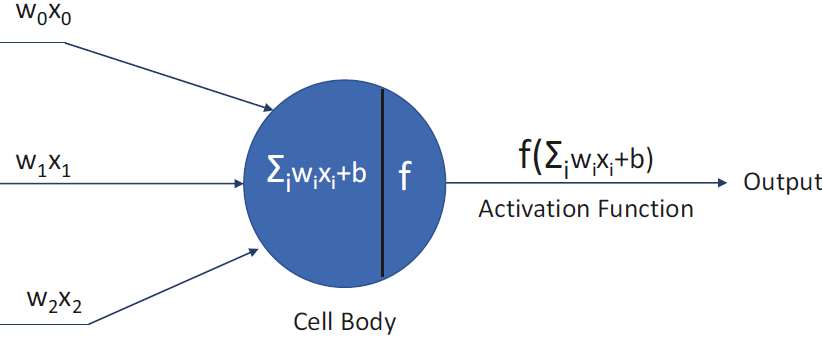
\includegraphics[scale=0.4]{pic/MA-Bilder/Neuron.PNG}
    \caption{Neuron, entnommen aus \cite{Verdhan.2020}}
    \label{Fig:neuron}
\end{wrapfigure}

\textbf{Das Neuron}

Als Grundbestandteil eines neuronalen Netzes übernimmt ein einzelnes Neuron die Aufgabe, Input eines vorangestellten Neurons zu empfangen und seinen eigenen Output zu berechnen, den es wiederum an ein weiteres Neuron weiterleitet. Wie in Abbildung \ref{Fig:neuron} illustriert, bildet ein Neuron seinen Output als Summe über alle Eingangswerte, wobei auch Gewichte der einzelnen Inputs beachtet werden und jeder Input ein anderes Gewicht haben kann \cite{Ertel.2021}. Diese Gesamtsumme der Inputs wird zusätzlich mit dem Bias-Term addiert, woraufhin das Gesamtergebnis in eine Aktiviierungsfunktion $f$ gegeben wird \cite{Ertel.2021, Verdhan.2020}. Der Einsatz verschiedenster Aktivierungsfunktionen ist im Kontext neuronaler Netze denkbar, wobei zu berücksichtigen ist, dass diese nicht-linear sein sollte. Beispiele für Aktivierungsfunktionen sind die \emph{Rectified Linear Unit}- (ReLU), die Sigmoid-Funktion oder die Softmax-Funktion, welche alle je nach Position innerhalb eines neuronalen Netzes und abhängig vom Problem, was es zu lösen gilt, unterschiedliche Vor- und Nachteile mit sich bringen \cite{Choo.2020}. Wurden innerhalb eines Neuron alle Inputdaten mithilfe der Aktivierungsfunktion bearbeitet, wird der erzeugte Output an das nächste Neuron weitergereicht und der Prozess wiederholt sich mit einem anderen Neuron \cite{Ertel.2021}.

\textbf{Strukturen neuronaler Netze}

Werden mehrere Neuronen gruppiert und verbunden, erhält man ein neuronales Netz. In einem simplen neuronalen Netz bilden die ersten und letzten Neuronen die sogenannte sichtbare Schichten, während die dazwischen liegenden Schichten als unsichtbare Sichten bezeichnet werden \cite{Choo.2020}. Bestehen Verbindungen zwischen den Schichten nur in eine Richtung, spricht man von einem \enquote{feed-forward}-Netzwerk \cite{Ertel.2021}. Ein solches ist in Abbildung \ref{Fig:neuronalesNetz} zu sehen. Bei der ersten Schicht handelt es sich um die Input-Schicht, welche die (u.U. vorverarbeiteten) Daten der Problemstellung entgegen nimmt. In dem Beispiel aus Abbildung \ref{Fig:neuronalesNetz} fließen die einzelnen Pixel des Bildes als Input in das neuronale Netz. Hierbei würde die Input-Schicht aus genau so vielen Neuronen bestehen, wie das Bild Pixel besitzt. Auf die Input-Schicht folgen verdeckte Schichten, in denen die Input-Daten nacheinander mithilfe der Neuronen transformiert werden. Die Output-Schicht als letzter Layer des neuronalen Netzes liefert das Vorhersageergebnis. Das Erscheinungsbild dieses Layers, also z.B. die Anzahl der Neuronen, ist vom zugrundeliegenden Problem und dessen Lösungsraum abhängig. In Bezug auf die verdeckten Schichten, sei angemerkt, dass mit der Anzahl der Schichten häufig auch die Präzision des Vorhersageergebnisses steigt, was jedoch zu Lasten des Rechenaufwandes geht \cite{Ng.2018}. Bei sehr vielen verdeckten Schichten spricht man häufig von DL, wobei nicht klar ist, wie viele Schichten ein künstliches neuronales Netz zu einem DL-Netz machen (vgl. Kapitel \ref{subsec_MLBegriff}). 

\begin{figure}
    \centering
    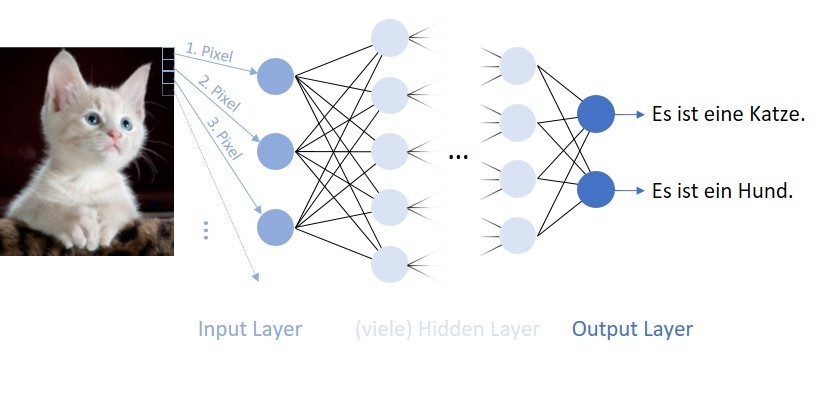
\includegraphics[scale=0.8]{pic/MA-Bilder/neuronalesNetz.jpg}
    \caption{Neuronales Netz entnommen aus \cite{MuellerKI}}
    \label{Fig:neuronalesNetz}
\end{figure}%

Neben dieser oben erläuterten Struktur neuronaler Netze existieren noch Abwandlungen, wie z.B. \emph{Convolutional Neural Network} (CNN) oder rekurrente neuronale Netzwerke \cite{Choo.2020}. Ein CNN lässt sich realisieren, indem dem neuronalen Netz nach der Input-Schicht eine oder mehrere Faltungsschichten (\emph{Conolutional Layer}) sowie \emph{Pooling}-Schichten hinzugefügt werden \cite{Ng.2018, Choo.2020}. Die Faltungsschicht hat zum Ziel lokale Muster zu finden, während das Pooling dafür verantwortlich ist, die Datenfülle zu reduzieren, da hierbei jedes Neuron nur die relevantesten Information an ihre jeweiligen Nachbarn weitergibt. CNNs werden häufig zur Bilderverarbeitung eingesetzt, da die Information, welche Pixel in einem Bild der Daten nebeneinander liegen, genutzt werden kann. Daneben existieren noch rekurrente neuronale Netzwerke als Sonderform der neuronalen Netze, welche besonders gut für die Analyse von zeitlichen Abfolge, wie z.B. Wetterdaten verwendet werden können. Hier wird nicht der gesamte Input auf einmal, sondern elementweise im Netzwerk verarbeitet. Zusätzlich verfügt jedes Neuron über einen eigenen Speicher, um Informationen über das vorherige Element nicht zu vergessen \cite{Choo.2020}.

\textbf{Training neuronaler Netze}

Beim Trainieren eines neuronalen Netzes steht die Anpassung der Gewichte und der Bias-Terme im Vordergrund. Da die Neuronen eigene Gewichte und eigenen Bias-Terme besitzen, besteht die besondere Herausforderung beim Trainieren darin, diese vielen, unterschiedlichen Parameter anzupassen. Zum Lernen wird eine Verlustfunktion (engl.: \emph{loss function}) eingesetzt, welche messen kann, inwieweit die durch das Netzwerk errechnete Antwort von der korrekten, realen Antwort abweicht \cite{Choo.2020}. Der Prozess der Anpassung der Gewichte und Bias-Vektoren selbst wird als \emph{Backpropagation} (dt.: Rückverfolgung) bezeichnet. Trifft das neuronale Netz eine falsche Vorhersage in der Output-Schicht, erfolgt eine Rückverfolgung des Fehlers und die Parameter werden insoweit angepasst, dass sich der Wert der Kostenfunktion reduziert, was wiederum eine Reduktion des inhaltlichen Fehlers zur Folge hat. Dieses Training wird meist in mehreren Runden durchlaufen \cite{Ng.2018}.

Das Potenzial der neuronalen Netze, welche das menschliche Gehirn abbilden, ist groß und bietet vielfältige Einsatzmöglichkeiten, während gleichzeitig bei der Implementation einige Herausforderungen bestehen. Analog zu den bereits betrachteten Verfahren, hängt die Funktionsweise stark von der Anzahl der vorhanden Trainingsdaten ab. Besonders, wenn das Netz komplexe Strukturen abbilden soll, und wenig Trainingsdaten vorhanden sind, neigt es zu Überanpassung \todo{Überanpassung ggf. einführen}. Weiter erfordert das Training neuronaler Netze einen hohen Rechenaufwand, der mit jedem zusätzlichen Neuron ansteigt. Ein weiterer Nachteil von neuronalen Netzen besteht darin, dass diese sich von Menschen nur schwer interpretieren lassen. Bei hundert Schichten mit mehreren Neuronen und individuellen Aktivierungsfunktionen sowie Parametern, lässt sich kaum nachvollziehen, wie ein neuronales Netzwerk zu seiner Vorhersage gelangt ist \cite{Ng.2018}. Eine Lösung für dieses Problem der Uninterpretierbarkeit bietet das erklärbare ML, das in folgenden Absätzen kurz dargestellt wird. 
\input{content/2_Theoretische Grundlagen/2_1_Maschinelles Lernen/2_1_5_Erklärbares maschinelles Lernen}

\section{Transparenz}
Dieses Kapitel definiert den Term "Transparenz", welcher im Mittelpunkt dieser Arbeit steht. Darauf folgend wird dargestellt, warum Transparenz speziell bei ML-System von großer Bedeutung ist.
\subsection{Definition}
\label{chap:Transparenz_Definition}
Der Begriff Transparenz kommt in den unterschiedlichsten Domänen vor, meint grundsätzlich jedoch, dass etwas durchschaubar oder nachvollziehbar ist \cite{DudenTransparenz}. Im ML-Umfeld hilft Transparenz dem in Kapitel \ref{subsec:XAI} beschriebenen Blackbox-Charakter entgegen zu wirken und lässt sich im Datenschutz-Umfeld \enquote{Klarheit, Erkennbarkeit und Nachverfolgbarkeit} verstehen \cite{bedner2010schutzziele, rudin2019stop}. Konkret sollten \enquote{Systeme [...] durchschaubar und ihre Funktions- und Arbeitsweise nachvollziehbar und verständlich} sein und die verarbeiteten Daten sowie die beteiligten Personen und Handlungen offenlegen \cite{bedner2010schutzziele}. Im XAI-Umfeld finden sich noch weitere Definitionen und Einordnungen des Begriffes der Transparenz. \cite{kamath2021explainable} stellen heraus, dass ein transparentes ML-Modell sowohl eine verständliche Struktur als auch einen verständlichen Algorotihmus besitzen muss. Transparenz ist eine Voraussetzung dafür, Modelle und deren Funktionsweisen zu verstehen. So sei an dieser Stelle erwähnt, dass Transparenz mit Erklärbarkeit (vgl. die Definition im vorangegangenen Kapitel \ref{subsec:XAI}) eng verwoben ist. Die Beziehung zwischen diesen Konzepten ist derart, dass sich Erklärbarkeit positiv auf Transparenz auswirkt \cite{kamath2021explainable}.
\subsection{Relevanz von Transparenz bei Algorithmen des maschinellen Lernens}
Transparenz ist insbesondere bei Algorithmen des MLs wichtig, da diese über einen stark ausgeprägten Black-Box-Charakter verfügen \cite{rudin2019stop}. Es kann jedoch gewünscht sein, nachzuvollziehen, wie und warum ein Algorithmus, eine Entscheidung getroffen hat \cite{fink2020quick}. Für diesen Wunsch nach Transparenz kommen verschiedene Motive unterschiedlichster Akteure in Frage. So ist es denkbar, dass es einem Entwickler wichtig ist, das System zu verstehen mit dem schlussendlichen Ziel dessen Funktionsweise zu verbessern. Daneben ist es für die Nutzer einer Software bedeutsam das System zu verstehen, um Vertrauen in die Technologie fassen zu können. Auch während der Nutzung eines Systems ist es von Vorteil, wenn das Verhalten des Systems nachvollziehbar bleibt, denn dies führt auch dazu, dass der Nutzer nicht zu einem Konkurrenzprodukt greift, was wiederum dem Softwarehersteller zugute kommt. Aber nicht nur für unmittelbar Systembetroffene ist Transparenz von Bedeutung, auch für die Gesellschaft ist es bedeutsam Stärken und Grenzen von Technologien einordnen zu können \cite{weller2019transparency}. Des weiteren rückt Transparenz in den Vordergrund, wenn Menschen fürchten, die Kontrolle über das eingesetzte System zu verlieren, was besonders im medizinischen Kontext fatale Folgen haben könnte \cite{fink2020quick, antoniadi2021current}. Aber auch im strafrechtlichen Umfeld, in dem Personen auf Grundlage von Entscheidungen eines Algorithmus Überwachung zu befürchten haben, wird Transparenz als ethisch und rechtlich notwendiges Gut betrachtet.Ferner ist auch ein nichtdiskriminierender Charakter gewünscht, welcher die Einhaltung der Grundrechte sichert \cite{EUVorschlag}. Auch lassen sich Systemverantwortliche oder das gesamte System mittels Transparenz leichter überwachen und in Bezug auf Sicherheitsstandards testen \cite{weller2019transparency, singh2018decision}. Überwachung des Systems ist z.B. bei selbstfahrenden Autos denkbar, in dem im Falle eines Unfalls Zurechenbarkeit und rechtliche Haftung ermöglicht werden soll \cite{weller2019transparency}.  Auch in einem Vorschlag der Europäischen Kommission \cite{EUVorschlag} findet sich die Forderung nach Transparenz besonders bei bestimmten Systemeinsatzkontexten (z.B. Deep-Fake-Systeme) wieder, um Manipulationsrisiken erkennen zu können. 

Die Forderung nach Transparenz ist jedoch nicht nur ein Motiv einiger Akteure, sondern bereits in bestehende Gesetze etabliert. Eine Forderung nach Transparenz bei der Datenveranverarbeitung findet sich in der Datenschutz-Grundverordnung (DSGVO) wieder. In Art. 15 DSGVO werden Privatpersonen beispielsweise die Rechte eingeräumt, Auskunft über die \enquote{Verarbeitungszwecke} sowie \enquote{die Kategorien personenbezogener Daten, die verarbeitet werden} einfordern zu dürfen. Die DSGVO fordert insbesondere in Artikel 12, dass \enquote{alle Informationen und [...] Mitteilungen [...], die sich auf die Verarbeitung beziehen, in präziser, transparenter, verständlicher und leicht zugänglicher Form in einer klaren und einfachen Sprache [übermittelt werden sollen]}.

Wenngleich viele, berechtigte Gründe für Transparenz innerhalb von ML-Systemen existieren, sei an dieser Stelle angemerkt, dass dies auch negative Folgen nach sich ziehen kann. So ist es möglich, dass Transparenz zu Lasten von Effizienz eingeführt wird, aber es ist auch denkbar, dass Transparenz eines Systems ausgenutzt wird, um ebendieses zu manipulieren oder die daraus gewonnenen Informationen unangemessen zu nutzen \cite{weller2019transparency}.

\section{Dokumentation von IT-Systemen}
Nach \cite{konigstorfer2021software} sind Dokumentation ein gutes Werkzeug zur Kommunikation und lassen sich gleichzeitig auch dazu einsetzen, ein System transparent, fair sowie zurechenbar zu machen. Sollen IT-Systeme Menschen näher gebracht werden, ist zunächst festzustellen, wer angesprochen werden soll. Im Umfeld der SW-Architektur-Dokumentationen stellen eine Art von Dokumentationen solche dar, welche für zukünftige Teammitglieder geschrieben sind, die aus dieser Motivation heraus das System verstehen wollen. Eine solche Dokumentation bietet darüber hinaus das Potenzial das System zu analysieren und zu verbessern. Neben der technischen Seite, sollten weiter verschiedene Stakeholder wie Nutzer, Auftraggeber oder Projektmanager beachtet werden, mit denen das System kommuniziert werden soll. Neben dem \emph{Wer} gibt es bei der Kommunikation von Systemen die Frage nach dem \emph{Was}. Grundsätzlich können einzelne Module, welche Teile von Software abbilden, Gegenstand von Dokumentationen sein. Auch kann die Performance z.B. als Fluss-Diagramm abgebildet werden. Weiterführend gibt es Unterschiede in der Art der Kommunikation. Diese ist informal durch die Unterstützung von Grafiken möglich, aber auch semiformal z.B. in Form eines UML-Diagramms \cite{bass2003software}. Die Standards im Bereich der Softwaredokumentation lassen sich nur bedingt auf selbstlernende Algorithmen übertragen \cite{rodvold1999software}. Im Rahmen der Handreichung in Kapitel tbd wird auf Besonderheiten bei Verfahren des maschinellen Lernens eingegangen.
\todo{Vlt. hier noch auf Besonderheiten bei ML eingehen?}

\chapter{Transparenzschaffende Maßnahmen aus der Literatur}
Im folgenden Kapitel ist der aktuelle Stand der Forschung dargestellt, welcher sich mit transparenzsschaffenden Maßnahmen im Umfeld des maschinellen Lernens beschäftigt. Die Erkenntnisse der Literaturrecherche bilden maßgeblich den Grundstein, für die zu erstellende Handreichung, die den Kern dieser Masterarbeit darstellt. Zunächst (in Kapitel \ref{sec:VorgehenLiteraturrecherche}) werden die Rahmenbedingungen dargelegt, an denen sich das Vorgehen orientierte. Darauf folgend werden in Kapitel \ref{sec:ErgebnisseLieratur} mit Blick auf die in Kapitel \ref{sec:ForschungszielundUmfang} formulierten Forschungsfragen die Ergebnisse der Literaturrecherche vorgestellt.

\section{Vorgehen der Literaturrecherche}
\label{sec:VorgehenLiteraturrecherche}
Unter einer Literaturrecherche versteht man das strukturierte Zusammentragen, Beschreiben und Erklären von wissenschaftlicher Literatur \cite{cooper_organizing_1988}. Hierbei können Methoden, Modelle oder Theorien im Vordergrund stehen, wogegen es eine Literaturrecherche gleichzeitig auch ermöglicht, den aktuellen Stand der Forschung zusammenzufassen. Somit lässt sich auch aufdecken, an welcher Stelle in einem Forschungsfeld noch Wissenslücken bestehen \cite{cooper_organizing_1988, Webster2002AnalyzingTP}.

\begin{figure}
    \centering
    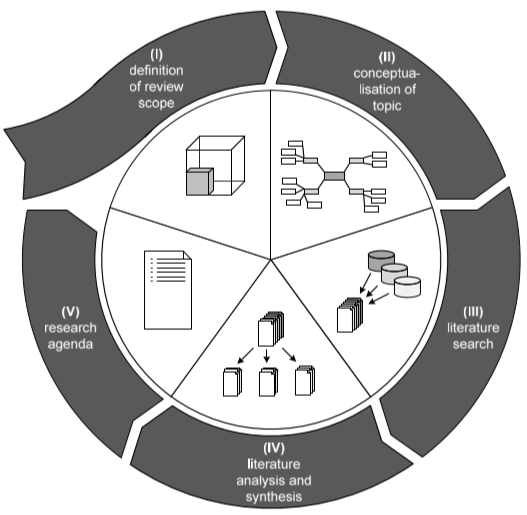
\includegraphics[scale=0.85]{pic/MA-Bilder/Model_vom_Brooke.PNG}
    \caption{Vorgehen einer strukturierten Literaturrecherche, entnommen aus \cite{vom_Brooke_2009}}
    \label{Fig:vomBrocke}
\end{figure}

Für eine Literaturrecherche stehen unterschiedlichste Vorgehensmodelle zur Verfügung. Diese Masterarbeit orientiert sich jedoch grob an dem Vorgehen von \cite{vom_Brooke_2009}, da dieses von mehreren wirtschaftsinformatiknahen Forschern im deutschsprachigen Raum entwickelt wurde. Die grobe Struktur des Vorgehensmodells ist in Abbildung \ref{Fig:vomBrocke} zu sehen. Die Literaturrecherche nach \cite{vom_Brooke_2009} umfasst die \emph{Definition des
Umfangs der Literaturrecherche}, \emph{Konzeptualisierung des Themas}, \emph{Literaturrecherche},
\emph{Literaturanalyse und -synthese} und \emph{Forschungsplanung}. Bei einzelnen Phasen der Literaturrecherche wird weiter noch auf Erkenntnisse von \cite{cooper_organizing_1988}, \cite{Brink.2013} und \cite{Webster2002AnalyzingTP} zurückgegriffen, was in den nachfolgenden Unterkapiteln erläutert wird.
\subsection{Definition des Umfangs der Literaturrecherche}
Um eine Abgrenzung des Umfangs einer Literaturrecherche vorzunehmen, empfehlen \cite{vom_Brooke_2009} die Taxonomie von \cite{cooper_organizing_1988}, welche in Abbildung \ref{tab:taxonomyCooper} dargestellt ist. Je nach Charakteristika kann sich während einer Literaturrecherche auf unterschiedliche Kategorien fokussiert werden. Die Entscheidungen, wo jeweils der Fokus liegen sollte, ergab sich meist aus der Aufgabenstellung. In der Abbildung \ref{tab:taxonomyCooper} ist durch Fettschrift hervorgehoben, welches Merkmal im Fokus lag, was folgend kurz begründet wird.

\begin{table}[h]
\begin{tabular}[h]{p{3.5cm}|p{8cm} l|l}
\large\textbf{Charakteristika} & \large\textbf{Kategorien} \\
\hline
Fokus & \begin{itemize}[nosep, leftmargin=*, before=\vspace{-0.5\baselineskip},after =\vspace{-\baselineskip}]
\item \textbf{Forschungsergebnisse}
\item Forschungsmethoden
\item Theorien
\item \textbf{Praktiken oder Anwendungen}
\end{itemize} \\
\hline
Ziel & \begin{itemize}[nosep, leftmargin=*, before=\vspace{-0.5\baselineskip},after =\vspace{-\baselineskip}]
\item \textbf{Integration}
\item Kritik
\item Identifikation zentraler Herausforderungen
\end{itemize} \\
\hline
Perspektive & \begin{itemize}[nosep, leftmargin=*, before=\vspace{-0.5\baselineskip},after =\vspace{-\baselineskip}]
\item \textbf{Neutral}
\item Bewertend
\end{itemize} \\
\hline
Umfang & \begin{itemize}[nosep, leftmargin=*, before=\vspace{-0.5\baselineskip},after =\vspace{-\baselineskip}]
\item Vollständig
\item Vollständig mit Selektion der Zitierungen
\item \textbf{Repräsentativ}
\item Zentral
\end{itemize} \\
\hline
Organisation & \begin{itemize}[nosep, leftmargin=*, before=\vspace{-0.5\baselineskip},after =\vspace{-\baselineskip}]
\item Historisch
\item \textbf{Konzeptuell}
\item Methodologisch
\end{itemize} \\
\hline
Zielgruppe & \begin{itemize}[nosep, leftmargin=*, before=\vspace{-0.5\baselineskip},after =\vspace{-\baselineskip}]
\item Spezialisierte Wissenschaftler
\item Generalisierte Wissenschaftler
\item \textbf{Praktiker}
\item Gesellschaft
\end{itemize} \\
\end{tabular}
\caption{\label{tab:taxonomyCooper} Umfang der Literaturrecherche, angelehnt an \cite{cooper_organizing_1988}}
\end{table}

\begin{enumerate}[label={(\arabic*)}]
    \item \textbf{Fokus:} Da eine Handreichung, welche sich im praktischen Kontext einsetzen lassen soll, primärer Gegenstand der Masterarbeit ist, legen eher Praktiken und Anwendungen im Fokus. Nichtsdestotrotz sollen auch Ergebnisse wissenschaftlicher Forschungen in die Gestaltung der Handreichung einfließen, da diese Handreichung im Rahmen einer wissenschaftlichen (Master-)arbeit entsteht.
    \item \textbf{Ziel:} Ziel der Literaturrecherche ist die Integration und Zusammenfassung verschiedener Methoden und Ansätze, welche in der Literatur existieren, um ein ML-System transparenter zu gestalten.
    \item \textbf{Perspektive:} Bei dem Zusammentragen verschiedener Maßnahmen wird eher eine neutrale Position eingenommen. Eine Wertung erfolgt jedoch (teilweise) in der Evaluation dieser Arbeit zu einem späteren Zeitpunkt.
    \item \textbf{Umfang:} Da in der Masterarbeit mehrere Forschungsfragen beantwortet werden müssen, in denen teilweise auf transparenzschaffende Maßnahmen mehrere ML-Verfahren eingegangen werden muss, wurde sich gegen eine vollständige Erfassung jeder zur Verfügung stehenden Literatur entschieden, um den zeitlichen Rahmen nicht zu sprengen. Stattdessen wurde eine repräsentative Recherche angestrebt, welche auf selektierten wissenschaftlichen Datenbanken aufbaut.
    \item \textbf{Organisation:} Die Rechercheergebnisse werden konzeptuell dargestellt.
    \item \textbf{Zielgruppe:} Die Ergebnisse der Literaturrecherche dienen vor allem der Erstellung der Handreichung, welche sich per Aufgabenstellung eher an Praktiker, wie z.B. die Entwickler von ML-Systemen richten soll.
\end{enumerate}
\subsection{Konzeptualisierung des Themas}
\label{chap:Konzeptualisierung}
Als zweiten Schritt sehen \cite{vom_Brooke_2009} vor, sich einen groben Überblick über das Thema zu verschaffen, um potenziell relevante Bereiche zu identifizieren. Hierfür wurde eine unstrukturierte Literaturrecherche durchgeführt, um Kernkonzepte zu finden, welche später den Grundstein für die strukturierte Literaturrecherche bilden, da durch diese relevante Suchbegriffe identifiziert werden konnten. Einige Kernaspekte standen nichtsdestotrotz durch die Aufgabenstellung bereits fest, aber um sich zusätzlich einen Überblick zu verschaffen, wurde der Suchbegriff \enquote{Transparency in Machine Learning} in die Datenbank Google Scholar eingegeben. 

In der folgenden Tabelle \ref{tab:suchbegriffe} sind die die Ergebnisse der Konzeptualisierungsphase, also die Suchbegriffe der strukturierten Literaturrecherche abgebildet. Nach \cite{Brink.2013} sind hierbei auch noch Synonyme, Ober- und Unterbegriffe sowie verwandte Begriffe miteinzubeziehen.

\begin{table}[!h]
\begin{tabular}[h]{p{4cm}|p{10cm} l|l}
\large\textbf{Gruppierung} & \large\textbf{Kernbegriffe} \\
\hline
Maschinelles Lernen & Machine Learning/ML, Künstliche Intelligenz/KI, Artificial Intelligence/AI, Erklärbares Maschinelles Lernen/Explainable Artificial Intelligence/XAI, Black-Box \\
\hline
Transparenz & Transparency, Verständlichkeit/Erklärbarkeit/Explainability, Interpretierbarkeit/Interpretability, DSGVO/GDPR, Zurechenbarkeit/Accountability \\
\hline
Methoden & Entscheidungsbäume/Decision Trees/Random Forest, k-means Clustering, Support Vector Machines, Logistische Regression/Logistic Regression, k-nächste Nachbarn/k-Nearest Neighbours, Bayessche Netze/Bayesian Networks, (Künstliche) Neuronale Netze/Artificial Neural Network/Deep Learning \\
\hline
Prozess & Process, Entwicklungslebenszyklus/Lebenszyklus/Entwicklung/Development Lifecycle/Lifecycle, Daten/Data, Datensatz/Dataset, Pipeline, Fluss/Flow \\
\end{tabular}
\caption{\label{tab:suchbegriffe}Suchbegriffe}
\end{table}

Um der Literaturrecherche eine auf die Forschungsfragen orientierte Struktur zu geben, wurden spezielle Suchterme definiert, welche teilweise individuell auf die jeweiligen Datenbanken zugeschnitten wurden und im Anhang zu finden sind. Während der Erstellung wurden die jeweiligen Begriffe zunächst probeweise in die Datenbank IEEE \footnote{https://ieeexplore.ieee.org/Xplore/home.jsp} eingegeben, um ungefähr abzuschätzen, welche und wie viele Ergebnisse erzielt werden. 

\textbf{Grundsätzliche transparenzschaffende Maßnahmen (RQ1)}
\begin{addmargin}[25pt]{0pt}
In Bezug auf die erste Forschungsfrage (\textit{RQ1: Wie können die unterschiedlichen Ebenen einer ML-Pipeline transparent gemacht werden?}) wurde zunächst versucht alle Begriffe der Konzeptualisierung in den Suchterm miteinzubauen. Jedoch brachte allein der Suchterm \enquote{Transparency AND ML OR DATA} bereits 1.338.968 Ergebnisse, was als unüberschaubar erschien. Aufgrund dieser sehr vielen Suchergebnisse wurde sich dafür entschieden, den Fokus auf den thematischen Kern dieser Masterarbeit zu legen, sodass für die erste Forschungsfrage der Suchterm \enquote{Transparency AND Machine Learning} gewählt wurde, da dieser auch schon zu genügend Ergebnissen führte.
\end{addmargin}

\textbf{Transparenzschaffende Maßnahmen konkreter ML-Verfahren (RQ2)}
\begin{addmargin}[25pt]{0pt}
Da der Fokus bei der zweiten Forschungsfrage (\textit{RQ2: Welche Ansätze existieren, um verschiedene ML-Algorithmen, wie z.B. Entscheidungsbäume oder auch neuronale Netzwerke zu erklären?}) eher auf den konkreten Methoden, welche innerhalb des ML-Lebenszyklusses eingesetzt werden liegt, wurde sich dazu entschieden, nach Möglichkeiten zu suchen, diese transparent, aber auch erklärbar zu machen. Der Aspekt des erklärbaren maschinellen Lernens wurde hier deswegen miteinbezogen, da in Kapitel \ref{chap:Transparenz_Definition} bereits herausgestellt wurde, dass Erklärbarkeit und Transparenz zusammenspielen. Somit wurde für den zweiten Forschungsaspekt nach dem jeweiligen Verfahren sowie nach Transparenz und Methoden der XAI gesucht. Für Entscheidungsbäume lautete der Suchterm beispielsweise: \enquote{decision tree AND Transparency AND XAI}.
\end{addmargin}

\textbf{Transparenzschaffende Maßnahmen je Zielgruppe}
\begin{addmargin}[25pt]{0pt}
In Bezug auf die dritte Forschungsfrage (\textit{RQ3: Inwieweit und auf welche Weise sollten ML-Algorithmen transparent gemacht werden, wenn diese Experten oder fachfremden Personen veranschaulicht werden?}) konnte während der Konzeptualisierung wenig konkretes gefunden werden, was als Suchterm sinnvoll erschien. In Absprache mit dem Betreuer dieser Masterarbeit wurde sich dazu entschieden, auf diese Forschungsfrage etwas weniger Gewicht zu legen als auf die anderen beiden. Inhaltlich wurden jedoch die Ergebnisse, welche sich mit dem anderen Suchthermen finden ließen, auch auf diese dritte Forschungsfrage hin geprüft.
\end{addmargin}
\subsection{Literaturrecherche}
Nach \cite{vom_Brooke_2009} steht im dritten Schritt des Vorgehens (vgl. \ref{Fig:vomBrocke} das Finden der Literatur an, indem Journal- und Wissensdatenbanken mittels Stichworten durchsucht werden, worauf folgend optional eine Vorwärts- und Rückwärtssuche durchgeführt werden kann.
Gesucht wurde im Juni und Juli 2022 auf Englisch in folgenden Datenbanken: IEEE, ACM \footnote{https://dl.acm.org/}, Computer Science Bibliography \footnote{http://dblp.uni-trier.de/} sowie Google Scholar \footnote{https://scholar.google.com/}. zusätzlich wurde noch die reguläre Suchmaschine \textit{Google} genutzt, da sich die Handreichung schließlich an Prakitker richten soll und somit auch Ansätze aus der Praxis, z.B. von Beratungshäusern oder großen Software-Firmen nicht ausgeschlossen werden sollten \todo{Das muss ich noch machen}.

Um die Anzahl der zu betrachtenden Publikationen und Beiträge überschaubar zu halten, wurden in wissenschaftlichen Datenbanken für RQ 1 die ersten 200 betrachtet. Da für die erste Forschungsfrage bereits viele wissenschaftlichen Quellen (296) gefunden wurde, die bereits auf Tranpsarenz bei konkreten ML-Methoden eingingen, wurde sich entschieden in Bezug auf RQ2 lediglich eine ergänzende Literaturrecherche durchzuführen, um zum einen keine relevanten transparenzschaffenden Methoden zu übersehen, jedoch zum anderen auf die Dokumentation aller gefundenen Literatur zu verzichten, um den zeitlichen und inhaltlichen Rahmen nicht zu sprengen.
- Google für transparenz in Machine Learning um keine in der Praxis relevanten Sachen zu verpassen (hierfür ersten 50 Ergebnisse von Websites)
- für RQ2: lesen des Titels und Abstract und dann Aufnahme in den Literaturpool (hierfür wurden die ersten 50 Ergebnisse von Google Scholar je Suchtherm  betrachtet)
- für die ergänzende Literaturrecherche wurden Duplikate nicht mit in die Dokumentation aufgenommen, sondern nur das was inhaltlich neu war


\begin{figure}
    \centering
    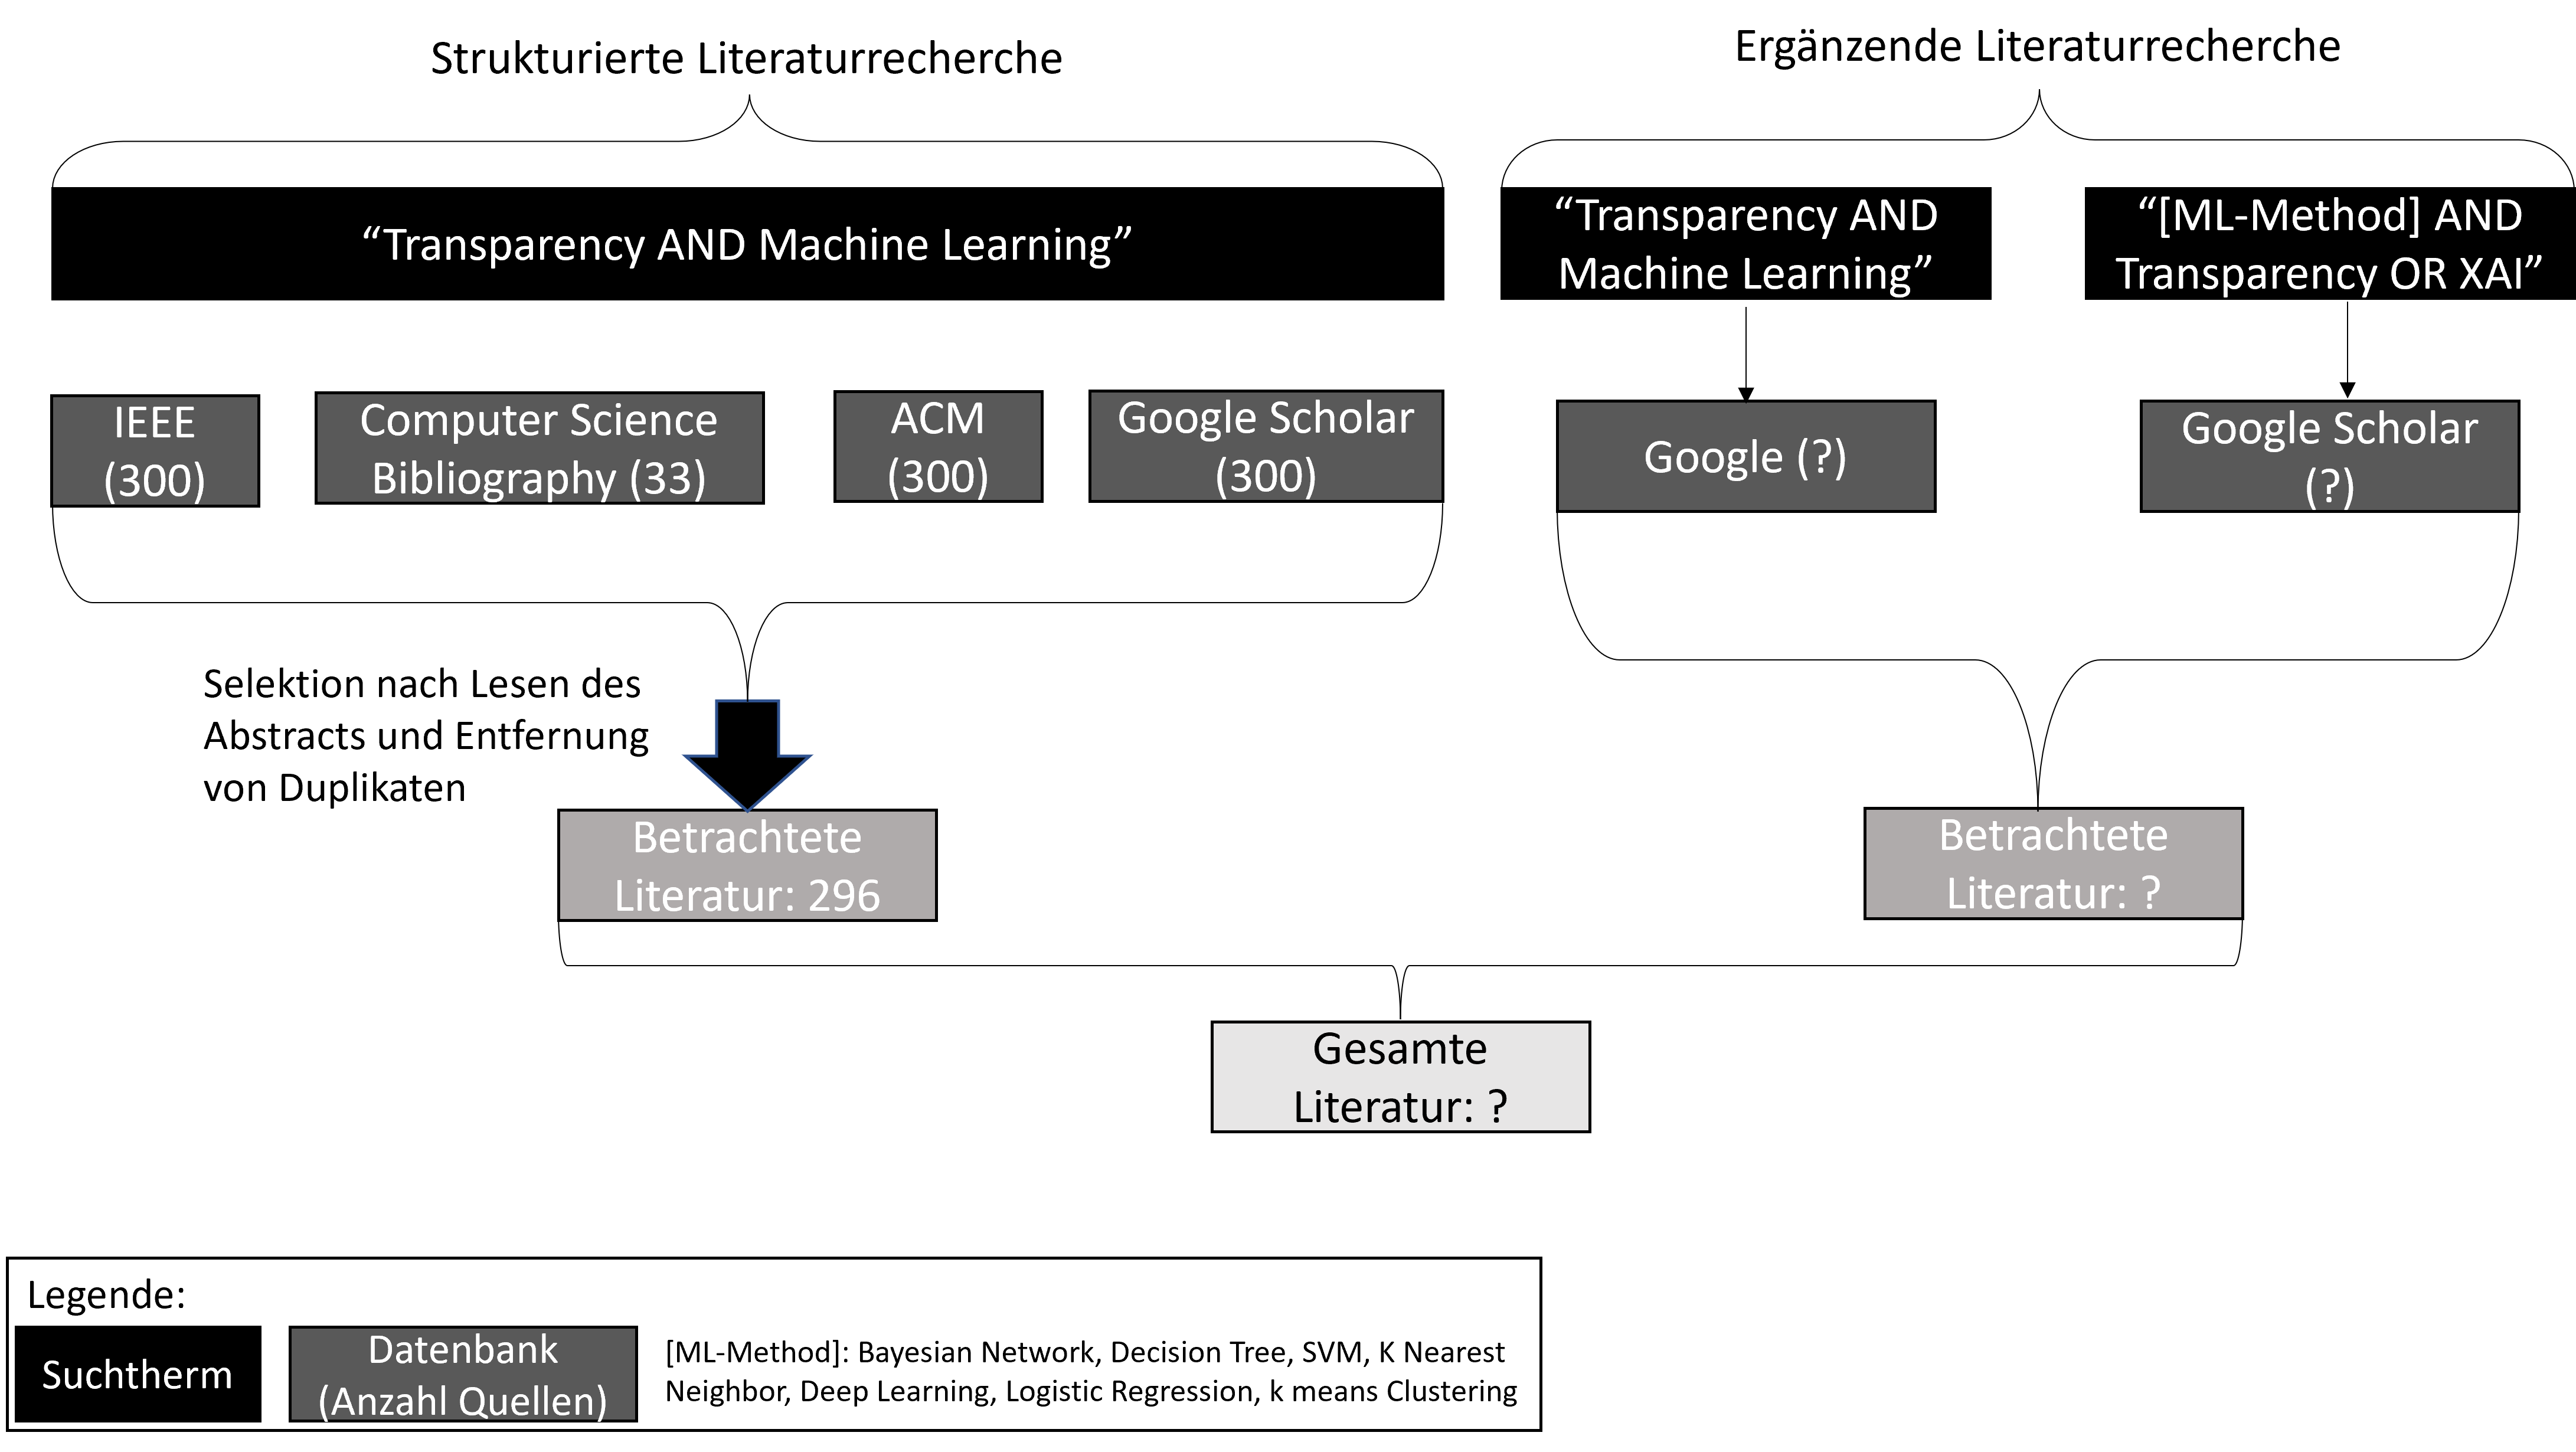
\includegraphics[scale=0.45]{pic/MA-Bilder/Literaturrecherche.png}
    \caption{Vorgehen bei der Literatursuche, eigene Darstellung}
    \label{Fig:Literatursuche}
\end{figure}

Eine Überblick über die verschiedenen Datenbanken, Suchterme und -ergebnisse findet sich im Anhang.
\subsection{Literaturanalyse und -synthese}
Teile der gefundenen Literatur wurde zunächst aussortiert. Hierfür wurden im ersten Schritt Duplikate entfernt, worauf folgend im zweiten Schritt die Literatur auf harte Kriterien geprüft wurde. Kriterien, welche hier Anwendung fanden, waren:
\begin{itemize}
    \item \enquote{Peer Reviewed Literature} (Veröffentlichungen in Jorunals oder Proceedings)
    \item Monographie/Buch
    \item Whitepaper
    \item Dissertationen
    \item Sprache: Englisch
\end{itemize}
Im dritten Schritt wurde der Titel und das Abstract der gefunden Beiträge näher betrachtet, um dessen Relevanz für Transparenz im ML einschätzen zu können. So wurden einige Paper aussortiert, die nicht wirklich dem Thema dieser Masterarbeit zuzuordnen sind und beispielsweise nur deswegen in der Suche erschienen, weil sie den Einsatz von ML-Technologien untersuchten, um eine Domäne wie z.B. die Finanzbranche transparenter zu machen. Zu betrachtende Quellen nach dieser ersten Reduktion waren 296 Quellen für RQ1.

das wurde mit dem zweiten Suchtherm nicht mehr gemacht, da hier ja von Anfang an nur die relevanten mit neuen Informationen dokumentiert wurden

Um diese viele Suchergebnisse noch weiter zu strukturieren, wurden die Quellen zunächst noch in grobe Kategorien eingeteilt. Beiträge, welche Transparenz und ML im Titel oder im Abstract behandelten, wurden als relevant klassifiziert, wenn diese auch konkrete Methoden betrachteten. Mit mittlerer Relevanz wurden solche Themen eingeordenet, welche eher den Fokus auf andere Themen legten (z.B. ethische oder rechtliche Behandlungen) legten, aber transparenzschaffende Maßnahmen betrachteten. Mit niedriger Relevanz wurden solche Quellen gekennzeichnet, welche Transparenz im Zusammenhang ML nur als Beispiel betrachteten. Sehr niedrig, wenn sie nur kurz erwähnten, dass etwas transparent ist. Zur inhaltlichen Abgrenzung kamen noch weitere Kategorien hinzu, welche sich zum Teil bereits im Vorhinein aus der Konzeptualisierung in Kapitel \ref{chap:Konzeptualisierung} ergaben, jedoch entstanden auch einige Kategorien neu nach Überfliegen der Literatur. So wurden beispielsweise Quellen identifiziert, welche nur bestimmte XAI-Methoden behandelten oder solche, die einen ganzheitlichen Ansatz zur Transparenz im ML darlegten oder sich nur auf Daten fokussierten.

\todo{Bei direkten Zitaten Seitenzahl? Joshua fragen}
\subsection{Forschungsagenda}
%Im meiner Recherche kam raus, dass es viele Methoden gibt, aber unklar ist wie gut die eingesetzt werden können, weil Faktor Mensch und dass zu Transparenz mehr gehört als XAI

%\cite{zhou20182d} sagt es gibt Resarch Gap, aktuell Konzentration nur auf die Entwicklung der Algorithmen, aber Rest unbeachtet. Sie sagen vor allem: Vorbereitung und Deployment sei wichtig

\section{Ergebnisse der Literaturrecherche}
\label{sec:ErgebnisseLieratur}
\subsection{Konzepte}
\label{subsec_Konzepte}
Mit Hilfe der Literaturrecherche konnten weitere Konzepte gefunden werden, welche im Forschungsgebiet des ML im Kontext der Transparenz definiert wurden. 

\subsubsection{Transparentes ML}
\label{subsubsec_TML}
\cite{zhou20182d} nennen das Konzept des transparenten maschinellen Lernens. Dies wird definiert als ML, welches es Nutzern ermöglicht die Entscheidungen des Algorithmus zu verstehen. Mit \textit{Nutzer} beziehen sich die Autoren insbesondere  auf solche Personen, welche nicht über Kenntnisse im Bereich des Trainieren von ML oder Mathematik verfügen. Transparentes ML bedingt mehrere positive Aspekte. Zum einen ermöglicht es Nutzern bessere Entscheidungen zu treffen und es wird sichtbar, ob ein System so funktioniert wie gewünscht. Im besten Falle ließen sich somit sogar Fehler und deren Ursachen aufdecken, was zu besseren Algorithmen führt. \textit{Besser} meint hier nicht im mathematischen Sinne optimiert, sondern den Einsatz von ML in der realen Welt. Des Weiteren stärkt tansparentes ML das Vertrauen. 

\subsubsection{Mensch und Maschine} 
Viele Autoren nennen die Zusammenarbeit von Mensch und Maschine als potenzielle Möglichkeit mehr Transparenz zu schaffen. Grundsätzlich lässt sich durch stärkere Intergation des Menschens in die gesamte ML-Pipeline mehr Transaprenz schaffen 
\cite{zhou20182d}.
Für die Zusammenarbeit von Mensch und Maschine existieren unterschiedliche Konzepte, das am meisten genannte heißt Human-in-the-Loop.
\todo[inline]{ Hier kommt noch eine Human-in-the-Loop Deinfition}
Neben den Vorteilen für Nutzer und Entwickler ergeben sich durch Human-in-the-Loop weitere positive Aspekte. Nach \cite{tam2016analysis} haben menschliche Inspektionen und Eingriffe in einen Klassifikationsalgorithmus im Vergleich zu einem traditionellen Algorithmus zu einer höheren Genauigkeit geführt.

\cite{wenskovitch2021beyond} erwähnt \emph{Human-Machine-Teams} als weitere Möglichkeit Transparenz zu schaffen. Hier arbeiten Menschen und Maschinen auf eine Art und Weise zusammen, in der die Maschine neue Muster erlernt und Menschen aufgrund dessen in der Lage sind neue Forschungsfragen und -hyptothesen zu bilden. Hierbei ist eine visuelle Schnittstelle essenziell für die Kommunikation vgl. Kapitel \todo[inline]{hier Referenz zu Vialsierungskapitel}. 
Auch \cite{westin2020building} weisen auf die Chance für Transparenz durch Human-Machine-Teams hin. Als weiterführende Literatur nennen sie hier z.B. das Modell für Human-Machine-Teams nach \cite{lyons2013being}, welches sich auf gemeinsame Absichten von Mensch und Maschine konzentriert. Weiter nennen sie noch \cite{chen2014situation}, welche das SAT(\emph{situation awareness-based agent transparency})-Modell entwickelt haben, bei dem das Bewusstsein für konkrete Situationen weiter in den Fokus gerückt wird.

\subsubsection{Mentale Modelle}
Im Rahmen der Literaturrecherche konnte herausgestellt werden, dass mentale Modelle, welche sich Nutzer über den Algorithmus bilden, wichtig für das Verständnis sind.
Ein mentales Modell besitzt nach \cite{kulesza2013too} unterschiedliche Ausprägungsformen, so kann zwischen dem strukturellen und dem funktionalen mentalen Modell unterschieden werden. Bildet sich eine Person ein strukturelles mentales Modell, gewinnt sie Erkenntnisse über die Funktionsweise eines Systems. Ein funktionales mentales Modell, hilft Menschen dabei ein System zu nutzen, während ein Verständnis über das System nicht notwendig ist.

\subsubsection{Facetten der Transparenz} 
\cite{vaughan2020human} stellen unterschiedliche Bausteine heraus, aus denen sich Transparenz zusammensetzt. So sei Traceability (dt.: Rückverfolgbarkeit) ein Teil von Transparenz, welcher die Dokumentation der gesteckten Ziele, die angewendeten Definitionen sowie das Systemdesign und die während der Entwicklung getroffenen Annahmen mit einschließt. Des Weiteren spielt die Kommunikation über den Zweck aber auch die Grenzen der AI eine große Rolle. Als dritten Baustein nennen sie Intelligibility (dt.: Verständlichkeit), welche Verständnis und Überwachung für Beteiligte ermöglichen soll. Um Verständlichkeit zu erreichen, spielen XAI-Methoden eine wesentliche Rolle.

\cite{huvc2021anomaly} fächern Transparenz anders auf und gliedern Transparenz in zwei Unteraspekte. Zum einen gibt es die funktionale Transparenz, welche beschreibt, wie ein Algorithmus funktioniert, und des Weiteren die Transparenz in Bezug auf die genutzten Daten.

Eine weitere Facette von Transparenz wurde von \cite{shin2020algorithm} herausgestellt. So beantworte Transparenz eher die Fragen, ob Daten legitimiert genutzt wurden und gibt weniger Auskunft darüber, ob der Algorithmus gut geeignet ist oder im mathematischen Sinne optimiert wurde.

\cite{siau2018building}Transparenz und Erklärbarkeit wirken sich positiv auf Vertrauen aus. \todo[inline]{Dieser Satz ist noch etwas einsam, vlt. solche Aspekte rauswerfen}
\subsection{Was transparent machen?}
\subsubsection{Inhaltlicher Kontext}
\cite{sendak2020human} stellten in ihrer Studie im medizinischen Umfeld heraus, solche Informationen mitzugeben, welche für das Publikum relevante Aspekte aufzeigen. So sollten sich Erklärungen auf den Kontext beziehen und sich auf Problemlösungen fokussieren \cite{sendak2020human}.

\subsubsection{Rahmenbedingungen und sozio-technischer Kontext}
\cite{cai2019hello} untersuchten im medizinischen Kontext, welche Informationen von Mitarbeitenden vor der Einführung eines ML-Systems gewünscht werden. Oberkategorien dieser gewünschten Informationen sind Möglichkeiten und Grenzen, Funktionalitäten, Subjektivität, Design-Ziele, Gedanken vor dem Einsatz.
\begin{itemize}
    \item In Bezug auf Möglichkeiten und Grenzen des Systems sollte kommuniziert werden, wie die grundsätzliche Performance des Algorithmus ist und worin dieser gute oder eben weniger gute Leistungen erbringt. Dies kann mithilfe von Leistungsmetriken angeben werden, in denen verdeutlicht wird, wie viele Datensätze richtig oder falsch klassifiziert wurden. Weiter sei für Nutzer interessant, wie sich der einzusetzende Algorithmus bei Fällen verhält, welche häufiger selbst von Menschen falsch eingeordnet werden. Auch sind die theoretischen Grenzen von KI grundsätzlich wichtig. Darüber hinaus sind die Trainingsdaten von Interesse. Hierbei ist die Diversität und Menge der Trainingsdaten wichtig, während sich auch das Datenformat (numerisch, binär, Bilder) von Bedeutung ist.
    \item In Bezug auf die Funktionalität wünschen sich Nutzer eine konkrete Beschreibung, über das, was der Algorithmus leistet. Hierbei steht zum einen der fachliche Kontext im Vordergrund, so nennen \cite{cai2019hello}, dass im medizinischen Kontext z.B. darauf hingewiesen werden könnte, ob ein Algorithmus \enquote{nur} dazu in der Lage ist Krebs zu erkennen oder noch weitere Krankheiten entdecken kann. Daneben ist auch der technische Kontext nicht uninteressant, so sei anzumerken, wie sich die Funktionsweise des Algorithmus im Vergleich zu der des Menschens unterscheidet. Für Bildklassifikation sei hier beispielsweise die Frage danach genannt, ob ein Algorithmus das Bild im Ganzen betrachtet oder ein Bild zunächst in einzelne Komponenten aufteilt und diese dann untersucht. Weiter ist von Interesse aus welcher Datenbasis heraus der Algorithmus die Entscheidung trifft. Des Weiteren ist bedeutsam für die medizinischen Praktiker, ob auch andere Daten des gleichen oder anderer Patienten in die Entscheidungsfindung miteinflossen.
    \item Da in der Praxis die Subjektivität einzelner Mediziner eine große Rolle spielt, ist die Subjektivität des Algorithmus wichtig für spätere Nutzer des ML-Systems. So ist es von Bedeutung Grenzfälle aufzuzeigen, welche auch von Menschen unterschiedlich bewertet werden. Hier interessiert die Praktiker der fachliche Hintergrund des Systems. Während der Einführung sollte außerdem die Möglichkeit bestehen, dass menschliche Praktiker ihre eigenen Diagnosen mit der der KI abgleichen können, um diese somit besser einschätzen zu können.
    \item Neben stark auf den Algorithmus selbst bezogenen Aspekte sprechen Nutzer auch den Design-Zielen eine hohe Bedeutung zu. So sei interessant, was der Nutzen des Systems in Bezug auf Kosten und Effizienz sei. Daneben ist wesentlich, ob die KI mit Menschen arbeiten soll oder unabhängig handelt.
    \item Weiterführend sind Gedanken vor dem Einsatz transparent zu machen. Diesbezüglich sollte kommuniziert werden, ob die rechtlichen und regulatorischen Rahmenbedingungen abgeklärt wurden oder ob eine behördliche Prüfung des Systems noch aussteht. Daneben wünschen sich Nutzer zu wissen, ob das Tool bereits schon von anderen Organisationen eingesetzt wird oder ob es im wissenschaftlichen Kontext auf seine Funktionweise hin überprüft wurde. Daneben stellt sich die Frage, ob es sich auf die täglichen Arbeitsabläufe der Praktiker auswirkt.
\end{itemize}

Ähnlich wie \cite{cai2019hello} wurde eine Studie von \cite{vorm2018assessing} durchgeführt, die untersuchte, was Menschen über das System wissen wollen, damit sie es als transparent erachten. Hierbei erarbeiteten \cite{vorm2018assessing} Faktoren und Beispielfragen in Bezug auf diese Faktoren. Zusätzlich erhoben die Autoren, wie wichtig einzelne Faktoren für Transparenz aus Nutzersicht wirken. In folgender Aufzählung\footnote{entnommen aus \cite{cai2019hello}, übersetzt mit kleinen Ergänzungen aus dem Fließtext des Papers} sind die Aspekte zusammengefasst.
\begin{itemize}
    \item Technische Faktoren:
    \begin{itemize}
        \item Daten (Wichtig): Wie aktuell sind die Daten, auf denen eine Entscheidung beruht?
        \item Unsicherheit (mittel): Trifft das System Annahmen aufgrund von unsauberen Daten?
        \item Logik (Wichtig): Was spricht für oder gegen die Entscheidung eines Systems? Woher kommt eine Entscheidung des Systems?
        \item Zuverlässigkeit (mittel): Unter welchen Bedingungen lag das System in der Vergangenheit falsch?
    \end{itemize}
    \item Persönliche Faktoren:
    \begin{itemize}
        \item Personalisierung (mittel): Wurde diese Empfehlung speziell für einen bestimmten Nutzer ausgesprochen?
        \item Vertrauen (Wichtig): Wie wird Vertrauen dieses System gemessen?
        \item Nachvollziehbarkeit (weniger wichtig): Was geschieht, wenn ein Nutzer die Entscheidung des Systems ablehnt?
    \end{itemize}
    \item Soziale Faktoren:
    \begin{itemize}
        \item Soziales Filtern (weniger wichtig): Wie ähnlich ist eine konkrete Person anderen Personen, welche auch diese Empfehlung erhalten haben?
    \end{itemize}
\end{itemize}
Ergänzen nennen \cite{vorm2018assessing} noch weitere Aspekte, die da wären:
\begin{itemize}
    \item Externe Abhängigkeiten: Mit welchen Daten arbeitet das System noch?
    \item Kritikalität: Die Bedeutung von Transparenz nimmt zu, wenn die Entscheidungen des Systems einen selbst oder andere beeinflussen.
    \item Rolle des Nutzers: Welche Informationen von Interesse sind hängt stark von der Rolle des jeweiligen Betrachters ab. So haben Entwickler, fachkundige Endnutzer sowie sekundäre Nutzer einen unterschiedlichen Fokus.
\end{itemize}

Diese zwei umfassenden Studien werden von anderen Wissenschaftlern weiter ergänzt und untermauert. So merken \cite{zhou20182d} an, dass das Kommunizieren von Unsicherheiten des Systems einen großen Teil zur Transparenz beitragen. Dies gilt jedoch nicht nur für Endnutzer des Systems, sondern nach \cite{gomez2021advice} sei auch für Modellentwickler interessant, was die Stärken und Schwächen des Modells sind, was auch durch das Aufzeigen von Fehlerfällen ausgedrückt werden kann.
\cite{irion2022algorithms} sprechen die Empfehlung aus nicht nur den Algorithmus, sondern auch soziale Aspekte und das gesamte System in die Kommunikation miteinzubeziehen.
\cite{goldenfein2019algorithmic} ergänzt, dass Transparenz auch Klarheit bei der Beschaffung und Umsetzung bedeute. Weiter sind Einfluss von Entscheidungen während der Nutzung von ML-Systemen von Bedeutung.
\subsection{Daten}
\subsubsection{Bias}
\todo[inline]{Bias/oder auch den ersten Teil des folgenden Abschnitts in mein Grundlagenkapitel mitaufnehmen?}
Bias in Daten ist ein großes Problem und kann sich negativ auf Fairness, aber auch auf die Funktionweise des ML-Algorithmus auswirken. Es existieren unterschiedliche Arten von Bias, welche an dieser Stelle kurz zusammengefasst sind \cite{suresh2021framework}: 
%Es existieren unterschiedliche Typen von Bias, welche zu unterscheidlichen Zeiptunkten auftreten können (siehe Figure 1 originalquelle).
\begin{itemize}
    \item Historischer Bias: Diese Art von Bias kann selbst dann entstehen, wenn Trainingsdaten optimal erhoben wurden. Schaden durch historischen Bias entsteht auch bei einer exakten Darstellung der realen Welt, jedoch existieren in dieser Stereotypen, welche im späteren Verlauf durch die Anwendung des Algorithmus weiter verstärkt werden könnten.
    \item Representation Bias ist eine Art des Bias, welche einen Teil der Bevölkerung unterrepräsentiert.
    \item Measurement Bias: Dieser Typ zielt auf Probleme bei der Auswahl, der Anhäufung und der Berechnung von Merkmalen und Zielvariablen ab. Dies kann durch begrenzte Möglichkeiten in der realen Welt bedingt sein, Daten exakt messen zu können.
    \item Aggregation Bias: Entitäten, welche in der Realität eigentlich unterschiedlich behandelt werden sollten, werden jedoch mit dem gleichen Modell behandelt.
    \item Learning Bias zielt auf falsche Modellierungsentscheidungen ab. So wird beispielsweise nicht die richtige Zielfunktion ausgewählt.
    \item Evaluation Bias: Die für die Evaluation genutzten Daten erfüllen keine oder andere Qualitätskriterien und -maßstäbe als die für das Training verwendeten Daten.
    \item Beim Deployment Bias steht die Problemlösung des Modells im Vordergrund. Das Modell erarbeitet seine Vorhersage auf eine andere Weise, als dies normalerweise getan wird, weil das Modell bspw. den sozialen Kontext unberücksichtigt lässt.
\end{itemize}

Um Bias zu erkennen, haben \cite{suresh2021framework} ein Framework entwickelt, welches es mithilfe von Formularisierung ermöglichen soll, Bias zu erkennen. \cite{suresh2021framework} verstehen den Datenverarbeitungsprozess als Aneinanderreihung von Mapping-Funktionen. Leider geben die Autoren keine Checkliste oder ähnliches an die Hand, um Bias erkennen zu können, weisen jedoch auf Aspekte hin, welche dabei helfen können. In folgender Aufzählung ist dies kurz zusammengefasst:
\begin{itemize}
    \item Historischer Bias: Wie sind Merkmale und Zielvariablen über die komplette Bevölkerung verteilt?
    \item Measurement Bias: Wie werden die Merkmale und Zielvariablen erstellt?
    \item Representation Bias: Kommt es zu Änderungen des Modells bei anderer Zielfunktion oder anderen Merkmalen?
    \item Aggregation Bias: Kommt es zu Änderungen durch das Wählen einer komplexen Zielfunktion oder anderen Trainingsdaten?
    \item Learning Bias: Kommt es zu Änderungen durch ein anderes Modell?
    \item Evaluation Bias: Kommt es zu Änderungen, wenn mehr als ein Datensatz oder mehrere Darebsätze zur Überprüfung genutzt wird?
    \item Deployment Bias: Dieser Typ ist schwer zu erkennen und aufzuheben, da dieser nur durch Experten aufgedeckt werden kann.
\end{itemize}

\subsubsection{Dokumentation der Daten}
Für die Dokumentation der Daten werden häufig sogenannte Datasheets empfohlen. Datasheets verfolgen den Zweck getroffene - eventuell unbemerkt getroffene - Annahmen aufzudecken. Diese Datasheets können darüber hinaus dabei helfen Fairness zu gewährleisten und die Leistung des ML-Systems zu optimieren \cite{vaughan2020human}. 
Beispiel für diese Datasheets sind z.B. nach \cite{vaughan2020human} Google Facets und Datasheets for Datasets.
Google Facets ist ein Visualisierungstool, was es ermöglicht Daten auf unterschiedlichen Granularitätsebenen zu untersuchen \cite{GoogleFacets}.
Datasheets for Datasets, entwickelt von \cite{gebru2021datasheets}, sind Datenblätter, welche für jeden Datensatz erstellt werden sollten und für die Dokumentation von Zusammensetzung, Sammlung, Motivation, der geplanten Verwendung, Verteilung und Pflege eingesetzt werden soll.
\cite{grasso2020applying} haben Datasheets for Datasets etwas abgewandelt für den Bereich der Biologie.
\todo[inline]{Hier gehe ich noch genauer auf die Datasheets-Arten ein und zeige vlt. Beispiele}

Merkmale, welche sich bereits in diesen Datasheets wiederfinden lassen, werden auch von anderen wissenschaftlichen Arbeiten herausgestellt. So betont \cite{de2018algorithmic}, dass für die Transparenz eines Datensatzes angegeben werden sollte, welche Merkmale vorhanden sind und wie diese z.B. über Frauen und Männer verteilt sind. Klassenungleichheiten sollten bei Datensätzen transparent gemacht werden.

Fairness kann auch mithilfe von Datendokumentation aufgedeckt werden, so könnte demonstriert werden wie und warum die Datensätze entstanden sind und warum ein konkreter Datensatz überhaupt ausgewählt wurde \cite{denton2020bringing}. In Bezug auf Fairness betonen jedoch \cite{de2018algorithmic}, dass es schwierig ist diskriminierende Merkmale überhaupt zu erkennen.

\subsubsection{Dokumentation der Datenverarbeitung}
Bevor ein Datensatz überhaupt genutzt werden kann, muss dieser häufig zunächst bereinigt werden. \cite{garbin2022assessing} empfehlen hier auch den Prozess der Bereinigung zu prüfen und auch festzuhalten, wie oder ob auf Bias in den Daten geprüft wurde. Beispielsweise kann angegeben werden, ob Zielvariablen korrigiert wurden.

\subsubsection{Transparenz über gleiche Datenformate}
\cite{huvc2021anomaly} empfehlen für den leichteren Überblick das Nutzen eines einheitlichen Datenformats. Hier nennen sie JSON oder XML als Optionen, wenngleich sie XML den Vorzug geben, da diese vollständige Schemata sowie Standardtransformationen ermöglicht.
\subsection{Transparenz durch das gewählte Modell}
Einige ML-Algorithmen gelten als in sich transparent. So liegt es auf der Hand, dass diese für transparentes ML eingesetzt werden können. 
Abbildung \ref{Fig:interpretierbarkeitJeModell} gibt einen guten Überblick, welche dabei hilft einzuordnen, ob ein Algorithmus leicht von Menschen verstanden werden kann.
\begin{figure}
    \centering
    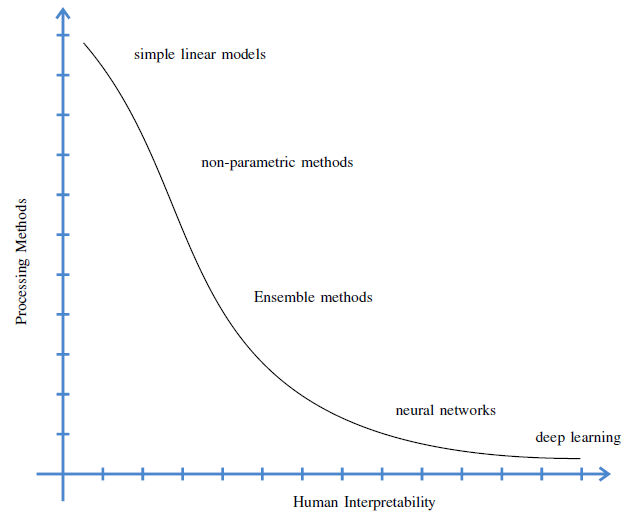
\includegraphics[scale=0.55]{pic/MA-Bilder/Literaturrecherche/48-InterpretierbarkeitJeModell.PNG}
    \caption{Interpretierbarkeit je nach Modell, entnommen aus: \cite{vorm2018assessing}}
    \label{Fig:interpretierbarkeitJeModell}
\end{figure}

\subsubsection{Transparente Modelle}
\label{subsubsec_transparenteModelle}
Folgend wird aufgelistet, welche Methoden als transparent gelten mit Bezug auf die jeweiligen Quellverweise.
\begin{itemize}
    \item Lineare Regression \cite{hanif2021survey, chen2021novel, palaniyappan2022aqx, ribeiro2016should}
    \item Logistische Regression \cite{hanif2021survey, schoeffer2022human, krause2017workflow, palaniyappan2022aqx, hill2018balancing}
    \item Entscheidungsbäume \cite{hanif2021survey, chen2021novel, krause2017workflow, de2018algorithmic, palaniyappan2022aqx}
    \item Random Forest \cite{chen2021novel, ribeiro2016should}
    \item Entscheidungsregeln (Wenn-Dann-Aussagen) \cite{hanif2021survey, chen2021novel}
    \item Generalized Linear Models (GLM) \cite{hanif2021survey}
    \item Generalized Linear Rules \cite{hanif2021survey}
    \item Generalized Additive Models (GAMs) \cite{hanif2021survey}
    \item Bayesche Regeln \cite{de2018algorithmic}
    \item k-nächste Nachbarn \cite{palaniyappan2022aqx}
\end{itemize}

In Bezug auf transparente Modelle sei angemerkt, dass einige dieser Methoden teilweise transparenter sind als andere. So geben \cite{hill2018balancing} an, dass logistische Regression leichter nachzuvollziehen sei als Random Forest, wenngleich Random Forests bessere Ergebnisse liefern. Ein weiterer wichtiger Aspekt ist, dass transparente Modelle (konkret von den Autoren genannt: logistische Regression und Entscheidungsbäume) zwar transparent seien, aber schwer zu generalisieren sind.

Daneben existieren noch weitere Ansätze von Wissenschaftlern, welche ihre eigenen transparenten Modelle entwickeln. Diese basieren jedoch meistens auf den Mechanismen, welche sich in den Methoden der obigen Listen wiederfinden lassen. 
Ein Beispiel für ein solches Modell sind fast-and-frugal-trees \cite{keller2020augmenting}, dessen Funktionsweise auf Entscheidungsbäumen basiert. Als besonderer Vorteil wird hier von den Autoren genannt, dass sich diese Art von Bäumen leicht visualisieren lässt und kein Hinzufügen nachträglicher Erklärungen (wie es bei Post-Hoc-Methoden der Fall ist) nötig ist. Somit ist eine Entwicklung mit einer solchen Methode zusätzlich weniger aufwendig.
Auch \cite{ainon2009transparent} entwickelten ein eigenes transparentes Klassifikationsmodell, indem sie mehrere transparente Methoden kombinieren, z.B. neuronale Netze und Wenn-Dann-Regeln. Diese erlauben eine transparente Abbildung des neuronalen Netzes. Dieses ist streng genommen keine neue Methode, sondern eine Anwendung von Global Surrogate \todo[inline]{Todo: Referenz auf Abschnitt im Kapitel der XAI-Methoden}

% das verstehe ich leider nicht: \cite{wang2005novel} eigene transparente Methode: feature decomposition method
\subsection{Modellauswahl}
Wie vorangegangen beschrieben existieren auch im ML-Bereich transparente Methoden. Um ein ML-Modell somit transparent zu machen, läge es also nahe einfach ein transparentes zu wählen, jedoch gibt es für diesen Ansatz Pro- und Contraargumente. 
Wird ein interpretierbares Modell gewählt, stößt man eventuell auf Grenzen, welche sich besonders bei nichtlinearen, komplexen Zusammenhängen oder einem Problemraum mit besonders vielen Merkmalen in den Trainingsdatensätzen zeigen \cite{hanif2021survey}.
Andere Autoren sehen jedoch in der Praxis eine andere Herangehenweise als zielführend an. Einfache Modelle funktionieren nicht unbedingt schlechter in der Realität. Vor allem in Branchen wie der Medizin oder Strafverfolgung, in denen Menschen das System gut verstehen sollten, kann es wünschenswert sein eine höhere Interpretierbarkeit als eine besonders gute Genauigkeit zu implementieren \cite{vaughan2020human, keller2020augmenting}.
\subsection{Erklärungen}
XAI- oder Visualisierungsmethoden können unterschiedliche Arten von Erklärungen produzieren. 

\cite{hernandez2021explainable} haben in einer Studie in der Luftfahrtbranche untersucht, welche Art von Erklärungen sich am besten eignen, um Vertrauen zu schaffen. Folgende Auflistung stellt die Ergebnisse da, wobei solche Erklärungen, welche am ehesten Vertrauen in die Technologie schaffen, in absteigender Reihenfolge genannt werden:
\begin{itemize}
    \item Wichtigste Faktoren, welche die Vorhersage beeinflussen
    \item Konkrete Beispiele für die Vorhersage
    \item Visuelle Darstellung der Funktionsweise
    \item Kausale Erklärungen (Welche Änderungen an den Eingabedaten oder am Algorihmus selbst würde eine andere Vorhersage ergeben?)
    \item Erläuterung des Lebenszyklus und des Entwurfs
    \item Kontrafaktische Erklärung (Warum ist die Vorhersage \enquote{A} und nicht \enquote{B}?)
\end{itemize}

Wenngleich \cite{hernandez2021explainable} herausgefunden haben, dass sich zumindest für das Vertrauen kontrafaktische Erklärungen weniger eignen, stellen \cite{tsiakmaki2021case} heraus, dass diese Art der Erklärungen Erkenntnisse liefern können, welche bei der praktischen Umsetzung während der Programmierung hilfreich sein können. Inbesondere liefern kontrafaktische Erklärungen ein gutes Verständnis über die Ursache-Wirkung-Beziehung.

\subsection{Einordnung von XAI-Methoden}
Für das Einordnen von XAI-Methoden existieren viele Ansätze, welche sich teilweise unterscheiden, aber auch Dinge gemein haben.

\cite{linardatos2020explainable} unterscheiden zwischen vier Oberkategorien mit mehreren Unterkategorien.
\begin{itemize}
    \item Zweck der Interpretierbarkeit (Anwendung eines White-Box-Modells, Post-hoc-Erklärungen eines Black-Box Modells, Sicherstellung von Fairness, Prüfen der Sensitivität von Vorhersagen)
    \item Modellspezifisch vs. Modellagnostisch
    \item Datentypen (Tabellen, Text, Bilder, Graphen)
    \item Lokal vs. Global
\end{itemize}

\todo[inline]{Hier schreibe ich dann, wie ich die einordne, wenn ich weiß, wie ich das machen will}
\subsection{XAI-Methoden für transparente Methoden}
Wenngleich transparente Modelle per Definition keiner Erklärung bedürften, wurden in der Literatur jedoch einige Methoden gefunden, welche zur Interpretation dieser eingesetzt werden können. Im folgenden Kapitel werden diese je Algorithmus präsentiert.

\subsubsection{Lineare Regression}
\cite{westin2020building} empfehlen für das Erklären des Outputs linearer Modelle die Hervorhebung der wichtigsten Eingabeparameter und deren relativen Bedeutung zueinander. 
\subsubsection{Entscheidungsbäume}
\cite{guidotti2018survey} empfehlen für die Erklärung von Entscheidungsbäumen eine Visualisierung dieser oder alternativ eine textuelle Erklärung in Form von Wenn-Dann-Regeln. Dies kann sowohl für lokale als auch globale Erklärungen angewendet werden.

\subsubsection{Random Forest}
Für das Erklären von Random Forests können Entscheidungsbäume und Wenn-Dann-Regeln eingesetzt werden. Hierbei kann ein Entscheidungsbaum globales Verständnis über den Random Forest bieten, während die Regeln der ungefähren Abbildung der Entscheidungen der einzelnen Bäume dienen sollen \cite{chen2021novel}.
%Hier auch: diese Methode ist nur Annäherung

\subsubsection{Sonstiges}
Die vorliegende Masterarbeit orientiert sich aus den in Kapitel \ref{subsubsec_Verfahren} genannten Gründen nur an einer Auswahl an ML-Methoden, für die XAI-Ansätze gesucht werden. In der Literaturrecherche wurden jedoch für andere Verfahren auch XAI-Methoden gefunden. Der Vollständigkeit halber werden diese hier aufgelistet. Auf weitere Erläuterungen wird jedoch verzichtet. 
\begin{itemize}
    \item GAM
    \begin{itemize}
        \item Gamut:interaktive Visualisierung mit der Zielgruppe: Data Scientists \cite{hohman2019gamut} 
    \end{itemize}
\end{itemize}
\subsection{Modellagnostische Methoden - lokal}
\todo[inline]{Was noch fehlt: Für welche Art von Problemen funktionieren diese Algorithmen? LIME nur für Klassifikation, aber die anderen? Vor- und Nachteile ausbauen...}

Folgendes Unterkapitel fasst eine Auswahl an Methoden zusammen, welche als modellagnostisch und lokale Ansätze einzuordnen sind (für eine Erklärung der Begriffe siehe Kapitel \ref{subsubsec:Erklaeransaetze}). Alle diese Ansätze, da sie modellagnostisch sind, haben gemeinsam, dass keine Zugriff auf die Modellstruktur notwendig ist. Es muss lediglich möglich sein Vorhersagen für Dateninstanzen abrufen zu können.

\subsubsection{LIME}
\label{subsubse_LIME}
Die Methode \emph{LIME}, entwickelt von \textcite{ribeiro2016should}, wurde in der betrachteten Literatur am häufigsten genannt (sieht z.B.: \cite{weitz2019you}, \cite{goldenfein2019algorithmic}, \cite{tsiakmaki2021case}, \cite{tjoa2020survey}, \cite{hanif2021survey}, \cite{krause2017workflow}, \cite{gomez2021advice}, \cite{wang2020explainable}, \cite{strobel2019aspects}, \cite{westin2020building}, ...)
LIME steht für \emph{Local Interptetable Model Agnostic Eplanations} und erklärt einzelne Vorhersagen eines jeden Klassifikationsalgorithmus, indem ein interpretierbares Modell lokal um eine zu erklärende Instanz herum gelernt wird \cite{ribeiro2016should}. Diese Erklärtechnik wird als lokaler Stellvertreter (eng.: \emph{Local Surrogate}) bezeichnet \cite{molnar2022}. 

%Dieses Modell ist meistens ein lineares Modell, was um die einzelnen Instanzen gebaut wird, die erklärt werden sollen. 
\textbf{Konzept}

Bei LIME kommt es zu einer lokalen Annäherung an ein Black-Box-Modell ($f$) durch ein zu interpretierbares Modell ($g$). Nach \textcite{ribeiro2016should} setzt LIME daher eine Abwägung zwischen Genauigkeit und Interpretierbarkeit voraus. Beispiel für interpretierbare Modelle sind in Kapitel \ref{subsubsec_transparenteModelle}) zu sehen.
In Abbildung \ref{Fig:Lime-Funktionsweise} sind die zwei Modelle $f$ und $g$ sowie verschiedene Instanzen zu sehen. Die rosa und die blauen Flächen demonstrieren die Funktionsweise des Black-Box-Modells, welche komplex und nicht-linear ist. Ziel von LIME ist es nun, zu erklären, warum eine bestimmte Instanz (das große rote Kreuz in der Mitte der Abbildung) in die Klasse \enquote{rosa} einsortiert wurde. Die LIME-Methode konzentriert sich nun als lokaler Ansatz auf den Bereich, um diese zu erklärenden Instanz. Um die zu erklärende Instanz herum werden nun zufällig weitere Datenpunkte erzeugt (Pertubationen). Dies ist durch die blauen Punkte und roten Kreuze dargestellt. Für diese Pertubationen, wird nun die Zielvariable mithilfe des Black Je näher sich diese Pertubationen an der zur erklärenden Instanz befinden, desto stärker fallen sie ins Gewicht. Nun wird sich mithilfe eines interpretierbaren Modell $g$ an dieser Instanz dem Black-Box-Modell $f$ angenähert. $g$ kann nun von Menschen interpretiert werden \cite{ribeiro2016should}. In der Abbildung würde ein Mensch also sehen, dass alles Werte links der gestrichelten Linie der Klasse \enquote{rosa} zuzuordnen sind. Alle Werte rechts der Linie, würden als \enquote{blau} klassifiziert werden. Hier wird noch einmal deutlich, dass LIME lediglich lokale Erklärungen erzeugt, denn Instanzen, welche sich auf dem Bild ganz links, weit entfernt der Entscheidungslinie befinden, gehören der blauen Klasse an. So ist die lokale Erklärung hier richtig, aber lässt global falsche Schlüsse zu.
\begin{figure}
    \centering
    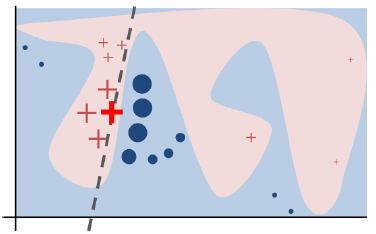
\includegraphics[scale=0.45]{pic/MA-Bilder/Literaturrecherche/LIME.PNG}
    \caption{Funktionsweise von LIME, entnommen aus: \cite{ribeiro2016should}}
    \label{Fig:Lime-Funktionsweise}
\end{figure}

\textbf{Formale Betrachtung}
Ziel von LIME ist das Finden des lokalen Stellvertreters, der lokal die eine bestimmte Instanz $x$ erklärt. Dieses Modell sollte so einfach wie möglich sein. Jedoch sind nicht alle Modelle gleich verständlich. So gibt es unterschiedliche Instanzen $g$ aus der Klasse $G$, die alle Instanzen von z.B. linearen Funktionen enthält. $G$ kann jedoch theoretisch auch die Menge aller Entscheidungsbäume sein \cite{ribeiro2016should}. So führen \textcite{ribeiro2016should} den Faktor  $\Omega(g)$ ein. Dieser misst die Komplexität eines interpretierbaren Modells, dies kann bei Entscheidungsbäumen beispielsweise die Tiefe eines Baums sein oder bei linearen Modellen die Anzahl an Gewichten. Nach \textcite{ribeiro2016should} kann nun eine Erklärung für den Datenpunkt $x$ durch folgendes Optimierungsproblem gefunden werden:
\begin{equation}
    \xi(x) = \underset{g \in G}{argmin} \mathcal{L}(f, g, \pi_{x}) + \Omega(g)
\end{equation}
$\mathcal{L}(f, g, \pi_{x})$ gibt an, dass eine gute Abschätzung an das Black-Box-Modell $f$ gefunden werden soll, welches sich in der Nachbarschaft $\pi_{x}$ befindet. Des Weiteren soll das gefundene Modell $g$ so einfach wie möglich sein, was durch $\Omega(g)$ angegeben ist \cite{ribeiro2016should}. Z.B. kann $\Omega(g)$ ausdrücken wie viele Merkmale von der interpretierbaren Funktion $g$ erfasst werden soll \cite{molnar2022}.
Um nun ein gutes Modell $g$ zu finden, muss der erste Therm der Formel optimiert werden. Hierfür wird sich die Nachbarschaft angesehen und dort lokal ein Modell gefunden. Ziel ist es das Modell mit der höchsten Genauigkeit zu finden. Dies geschicht, indem für alle Datenpunkte in der Nachbarschaft aus Abbildung \ref{Fig:Lime-Funktionsweise} sowohl das interpretierbare Modell $g$ als auch das Black-Box Modell $f$ aufgerufen wird. $g$ wird nun daraufhin optimiert, so wenig Fehler wie möglich zu haben, was mit den Vorhersagen des Black-Box-Modells überprüft werden kann. Bei diesem Optimierungsproblem fallen Punkte, die näher an $x$ liegen stärker ins Gewicht. 
%Diese Formel kann mit verschiedenen Erklärungen $G$, Funktionen $\mathcal{L}$ oder Komplexitätsmaßen $\Omega$ genutzt werden.

%So sind nicht alle interpretierbaren Modelle (vgl. Kapitel \ref{subsubsec_transparenteModelle}) im gleichen Maße für Menschen verständlich. \textcite{ribeiro2016should} definieren in ihrem Paper eine Erklärung als $g \in G$, wobei $G$ alle interpretierbaren Modelle (z.B. Entscheidungsbäume oder lineare Modelle) enthält. 
%Bevor eine Erklärung von LIME präsentiert wird, werden zunächst kurz Grundlagen bzgl. der Interpretierbarkeit von Modellen erläutert. Zuallererst ist es wichtig, sich den Unterschied zwischen Merkmalen, welche das Black-Box-Modell verwenden, und für Menschen interpretierbaren Daten zu verdeutlichen. \textcite{ribeiro2016should} demonstrieren dies mit einem Beispiel aus der Texklassifikation. Ein binärer Vektor, der beschreibt, ob sich ein bestimmtes Wort in einem Text befindet und somit zur Klassenvorhersage führte, ist für den Menschen interpretierbarer als die Datenstruktur, welche durch den Algorithmus in Wahrheit (z.B. Wordembeddings) zur Bearbeitung der Klassifikationsaufgabe genutzt wird. Formal definieren sie $ x \in \mathds{R}^{d}$ als originale Repräsentation, während $ x' \in \{0,1\}^{d'}$ die binäre Repräsentation ist, welche für Menschen interpretierbar ist. 

%\begin{figure}[h]
%    \centering
%    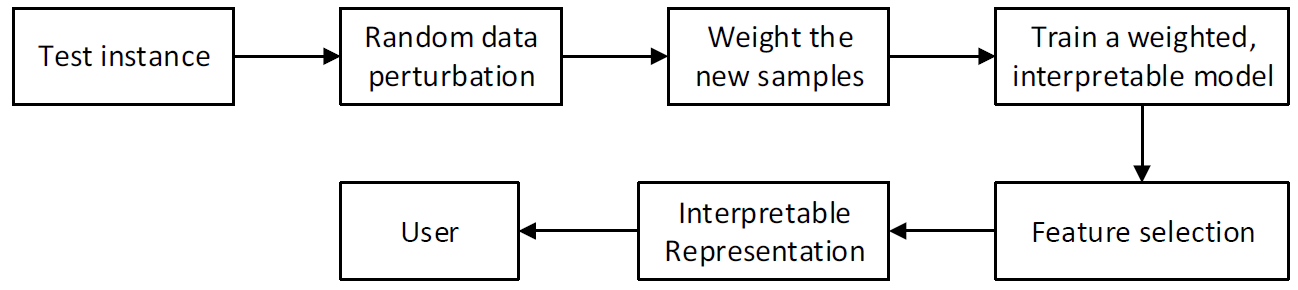
\includegraphics[scale=0.45]{pic/MA-Bilder/Literaturrecherche/LIME-Ablauf.PNG}
%    \caption{Ablauf von LIME, entnommen aus: \cite{zafar2019dlime}}
%    \label{Fig:Lime-Ablauf}
%\end{figure}

%\cite{kamath2021explainable}: der Verlust von $\mathcal{L}$ wird nun abgeschätzt, indem zufällige Pertubationen $z$ um die Instanz die erklärt werden soll erzeugt werden. Diese Datensätzen werden gewichtet mithilfe von $\pi_{x}(z)$, um die Distanz zu bestimmen.

\textbf{Anwendung von LIME}

Ein Beispiel für eine mit LIME erzuegte Erklärung ist in Abbildung \ref{Fig:Lime-Beispiel} dargestellt. Hier wurde anhand verschiedener Werte untersucht, ob eine Person Diabetes hat. Hier wurde eine Person mit einer Wahrscheinlichkeit von ungefähr 60 (links dargestellt) als Diabetes-Patient eingeordnet. Diese Entscheidung wird vor allem durch die orange dargestellten Merkmale unterstützt, so z.B. das Alter. Blau markiert sind solche Merkmale, welche eher für einen gesunden Patienten sprechen würden. Rechts sind zur Übersicht die Merkmalswerte aufgezeigt.
\begin{figure}
    \centering
    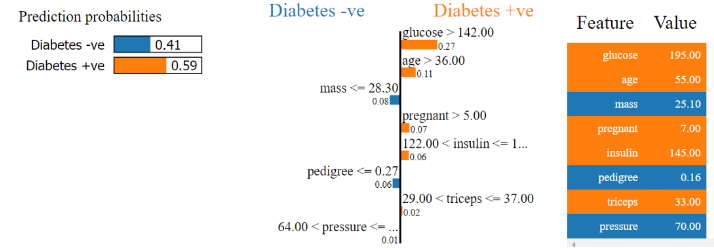
\includegraphics[scale=0.45]{pic/MA-Bilder/Literaturrecherche/LIME-Erklaerung-Beispiel.PNG}
    \caption{Erklärung der Klassifikation einer bestimmten Instanz, entnommen aus \cite{LIME-beispiel}}
    \label{Fig:Lime-Beispiel}
\end{figure}
Zur praktischen Umsetzung von LIME stellen die Erfinder eine Bibliothek\footnote{https://github.com/marcotcr/lime} zur Verfügung. LIME kann für jeden Klassifikationsalgorithmus auf tabellarischen Daten, Text oder auch Bilder angewendet werden. Weiter kann durch den Entwickler ausgewählt werden, wie viele Merkmale dargestellt werden sollen \cite{molnar2022}. Je nach dem, welche Daten dem Klassifikationsalgorithmus zu Grunde liegen, kommt es zu leichten Unterschieden in der Anwendung. So muss zwischen Merkmalen, mit denen ein Algorithmus arbeitet und Merkmalen, welche für Menschen interpretierbar sind, unterschieden werden \cite{ribeiro2016should}. \textcite{ribeiro2016should} demonstrieren dies mit einem Beispiel aus der Texklassifikation. Ein binärer Vektor, der beschreibt, ob sich ein bestimmtes Wort in einem Text befindet und somit zur Klassenvorhersage führte, ist für den Menschen interpretierbarer als die Datenstruktur, welche durch den Algorithmus in Wahrheit (z.B. Wordembeddings) zur Bearbeitung der Klassifikationsaufgabe genutzt wird \cite{ribeiro2016should}. Bei Textklassifikation werden nun Permutationen dadurch erzeugt, dass zufällig Wörter aus einem Text etfernt werden. Die Klasse wird danndamit erklärt, ob oder wie oft ein bestimmtes Wort in einem Text vorkam.

\textbf{Vor- und Nachteile}

Die Formel von LIME kann mit unterschiedlichen ML-Methoden von $f$ und $g$ genutzt werden \cite{ribeiro2016should}. Dies bedeutet, das zugrundeliegende Black-Box Modell kann ausgetauscht werden, während der lokale Stellvertreter $g$ nicht geändert werden muss. Auch kann ein lokaler Stellvertreter genutzt werden, welchen die Erklärungsbetrachter gut verstehen, weil schon Vorwissen vorhanden ist (z.B. Entscheidungsbäume) \cite{molnar2022}. 
\textcite{ribeiro2016should} stellen in ihrer Veröffentlichung besonders heraus, dass LIME Vertrauen in ML-Algorithmen erhöhen kann und zur Erkennung von unerwünschten Verhalten beiträgt. So weisen sie auf einen Klassifikationsalgorithmus hin, welcher Fotografien von Wölfen und Huskys unterscheiden sollte. LIME ermöglichte es, aufzudecken, dass dieser Algorithmus solche Bilder mit Schnee im Hintergrund, der Klasse Husky zuordnete und die Tiere selbst gar nicht beachtete \cite{ribeiro2016should}.

Nachteil ist die Schwierigkeit bei tabellarischen Daten, die Nachbarschaft zu bestimmen \cite{molnar2022}. Weiter entdeckten \textcite{slack2020fooling} eine Möglichkeit, dass sich Erklärungen manipulieren lassen um Bias in den Daten zu verstecken, was zu Vertauensverlust führen kann.  Daneben werden die Daten immer zufällig generiert, sodass gleiche Instanzen unterschiedliche Erklärungen erhalten können. Dieses Problem löst eine Abwandlung von LIME. \textcite{zafar2019dlime} entwickelten DLIME (\emph{Deterministic Local Interpretable Model-Agnostic Explanations Approach for Computer-Aided Diagnosis Systems}). Hier werden die Pertubationen anders generiert (agglomeratives hierarchisches Clutering) und für die Auswahl der sich der zur erklärenden Instanz am nächsten befindlichen Datenpunkte den in Kapitel \ref{subsubsec_KNN} beschriebenen KNN-Algorithmus nutzen.

\subsubsection{SHAP}
Auch die modellagnostische Methode \emph{SHAP} wurde von vielen Autoren genannt (\cite{tsiakmaki2021case}, \cite{vaughan2020human}, \cite{schoeffer2022human}, \cite{hanif2021survey}, \cite{gomez2021advice}, \cite{wang2020explainable}, \cite{palaniyappan2022aqx}, ...). Diese Methode wurde zuerst von \textcite{lundberg2017unified} vorgestellt und basiert auf den sogenannten SHAPLEY-Werten aus der Spieltheorie. SHAPLEY-Werte beantworten die Frage, was ein einzelner Spieler innerhalb einer Gruppe beitrug. Angewendet auf das Forschungsfeld des MLs können einzelne Spieler als Merkmalswerte betrachtet werden\cite{wang2020explainable}.

\textbf{Konzept}

Die Shapley-Werte wurden von \textcite{shapley1951notes} eingeführt. Gegeben ist eine Gruppe von Spieler, welche gemeinsam einen Wert $v$ erzielen. In dem Beispiel von \textcite{molnar2022} ist dies ein Preis für eine Wohnung. Verschiedene Spieler oder im ML-Kontext Merkmale wirken sich unterschiedliche auf einen Wohnungspreis aus. Beispielhafte Merkmale können hier das Stockwerk, die Lage oder das Verbot von Haustieren sein. Um nun den Beitrag eines Merkmals zu berechnen, kann nun getestet werden, welchen Wohnungspreis ohne ein bestimmtes Merkmal erzielt werden würde. Nun wird dieses Merkmal, z.B. das Haustierverbot, ausgeklammert und der Wohnungspreis berechnet. Dies muss für alle Kombinationen, wo das Haustierverbot fehlt, geschehen, um Abhängigkeiten zwischen Merkmalen zu erkennen. Nun wird die Differnez zwischen dem ursprünglichen Wert $V$ und dem neuen Ergebnis berechnet. Über alle Ergebnisse wird der Durchschnitt gebildet. Dies geschieht für alle anderen Merkmale analog. Somit erhält man die Shapley-Werte für alle Merkmale \cite{molnar2022}.

\textbf{Formale Betrachtung}
textcite{lundberg2017unified} wenden dieses Konzept in ihrer Methode (SHAP (\emph{SHAPLEY ADDITIVE EXPLANATIONS})) an, um einzelne Vorhersagen zu erklären, indem Beiträge eines jeden Merkmals berechnet werden. Sei $x$ die zu erklärende Instanz und $f(x)$ das Black-Box-Modell. Zu $x$ existieren noch vereinfachte lokale Eingabe $x'$. Dieses muss eingeführt werden, um die Werte der Merkmale zu vereinfachen, so werden sie z.B. als binäre Vektoren dargestellt. Weiter existiert für das Black-Box-Modell ein Modell $g$, für das gilt $g(x') \approx f(x)$. $g$ sieht weiter wie folgt aus und gibt an, was ein Merkmal zu einer Vorhersage einer Instanz $x'$ beiträgt (vereinfacht von \cite{Gianfagna.2021} nach \cite{lundberg2017unified}):
\begin{equation}
    g(x') = \phi_{0} + \sum\limits_{i=1}^{M}\phi_{i}x'_{i}
\end{equation}
Mit $\phi_{0}$ ist der sogenannte \emph{Null-Output} und meint den durchschnittlichen Output des Modells, den von den einzelnen Merkmalen unabhängig ist. $i$ ist ein Merkmal und $M$ ist die Anzahl aller Merkmale. $\phi_{i}$ ist der Erklärungseffekt eines Merkmals $i$ und gibt an, wie viel dieses Merkmal zu einer Veränderung der Vorhersage beiträgt \cite{lundberg2017unified}. 


\textbf{Anwendung}
\textcite{lundberg2017unified} stellen eine Bibliothek\footnote{https://shap.readthedocs.io/en/latest/index.html} für die Nutzung von SHAP zur Verfügung. Dort ist auch aufgelistet, worfür SHAP verwendet werden kann, z.B. für Klassifikation oder Regression. Ein Beispiel für eine mit SHAP generierte Erklärung ist in Abbildung \ref{Fig:Beispiel_Shap} dargestellt. Hier wird die Ausgabe des Wertes 0,4, welche durch ein Black-Box-Modell erstellt wurde, erklärt. Merkmale, welche die Vorhersage in einen höheren Wert ändern, wie z.B. das Alter, sind rot eingezeichnet. Blau eingezeichnete Merkmale, wie z.B. das Geschlecht würden den Wert der Vorhersage verringern.
\begin{figure}
    \centering
    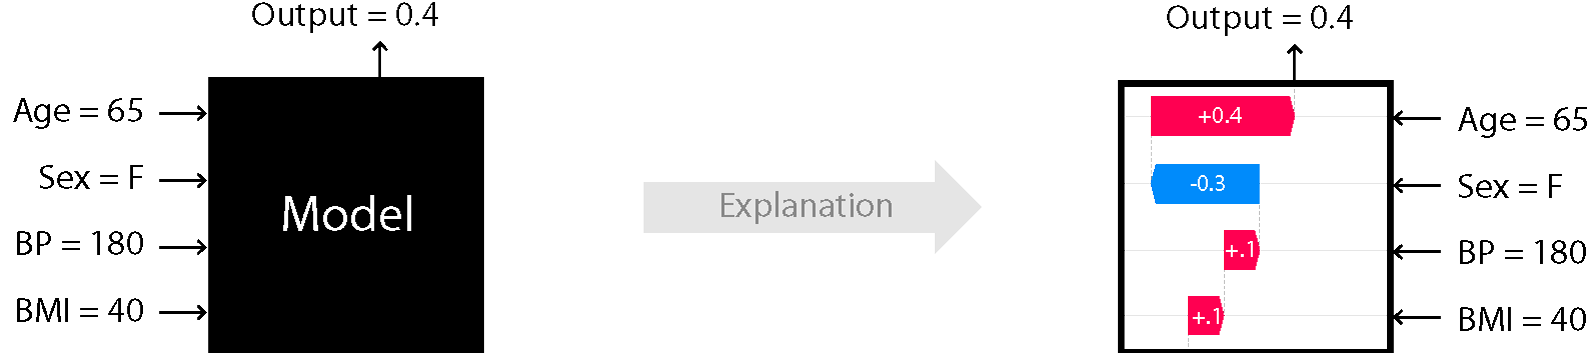
\includegraphics[scale=0.45]{pic/MA-Bilder/Literaturrecherche/SHAP-Beispiel.PNG}
    \caption{Beispiele Erklärungen mit SHAP, entnommen aus der SHAP Bibliothek}
    \label{Fig:Beispiel_Shap}
\end{figure}
Ein praktisches Problem mit SHAP besteht in der Berechnung der SHAPLEY-Werte. Würden 4 Features vorliegen, müssen 16 verschiedene Möglichkeiten für die Exkludierungen der Features berechnet werden. Bei 32 Features, wären dies schon 17,1 Milliarde Berechnungen. Hierfür haben \textcite{lundberg2017unified} den Shapley Kernel entwickelt, welcher sich SHAPLEY-Werte annähert und weniger Datensätze erstellen muss. Für Kernel SHAP definieren die Autoren auch Sonderformen, wie z.B. Deep SHAP für DL, welche sich die Funktionsweise der zugrunde liegenden ML-Modelle zunutze machen.
SHAP kann weiterhin auch für globale Erklärungen verwendet werden, wenn diese für jede Instanz angewendet wird \cite{molnar2022}.

\textbf{Vor- und Nachteile}
Nach \textcite{lundberg2017unified} grenzen sich SHAP-Erklärungen von anderen Erkläransätzen ab, da sie drei wichtige Eigenschaften erfüllen: lokale Genauigkeit, Fehlen, Konsistenz.
Als erste wünschenswerte Eigenschaften wird lokale Genauigkeit definiert, so muss das Erklärungsmodell $g$ das Black-Box-Modell $f$ approximieren, sodass auch die Ausgaben von $f$ und $g$ ungefähr übereinstimmen. Des Weiteren sollten auch die Werte der Erklärungen 0 für nicht vom Modell betrachtete Features sein (Eigenschaft: Fehlen). Die dritte Eigenschaft ist Konsistenz \cite{lundberg2017unified}. So sollte eine Zunahme (oder Gleichbleiben) eines Merkmalswertes bedingen, dass auch der SHAPLEY-Wert zunimmt (oder gleich bleibt). Weiter basiert SHAP auf einer soliden wissenschaftlichen Grunglage und beziehen bei ihrer Erklärung alle Merkmale mit ein. Laut \textcite{molnar2022} macht sie dies zu einer geeigneten Methode, das Recht auf Erklärungen der DSGVO umzusetzen. Daneben können sowohl lokale als auch globale Erklärungen generiert werden \cite{molnar2022}. Ein Nachteil dieser Methode besteht jedoch auch in den Shapley-Werten an sich. Da sie immer jedes Merkmal beachten, sind Shapley Werte, die falsche Wahl, wenn dem Nutzer nur einige wenige Merkmale präsentiert werden sollen. Hier sei LIME besser geeignet, da hier die Reduktion auf einige wenige Merkmale möglich ist.
Ein weiterer Nachteil, der jedoch auch für LIME gilt, sit die von \textcite{slack2020fooling} entdeckte Manipulationstechnik, welche angewendet werden kann, um Bias in den Daten zu verstecken. Weiter ist auch die Berechnung mit dem SHAP-Kernel recht langsam und aufwendig \cite{molnar2022}.

\subsubsection{Anchors}
Die folgende Methode wurde von den selben Wissenschaftlern entwickelt, welche auch LIME vorgestellt hatten und produziert Wenn-Dann-Regeln, die \enquote{Anchors} genannt werden \cite{ribeiro2018anchors}.

\textbf{Konzept}
Der folgende Ansatz setzt auf einer Schwäche der LIME-Methode auf. Wie in \ref{subsubse_LIME} beschrieben, werden Erklärungen mittels LIME durch lokale Annäherungen an bestimmte Instanzen produziert. In der Abbildung \ref{Fig:Lime-Funktionsweise} wurde gezeigt, dass alles lokal links der Entscheidungslinie der rosa Klasse zuzuordnen war, wenngleich sich links, weiter entfernt der Entscheidungslinie Instanzen befanden, welche als blau zu klassifizieren sind. LIME beantwortet also nicht die Frage, für welche Instanzen ihre Erklärung übertragbar ist. Dieses Problem wird von \textcite{ribeiro2018anchors} allerdings mit Hilfe der Anchors adressiert.
In Abbildung \ref{Fig:Funktionsweise_Anchors} sind die Funktionsweise von LIME und Anchors zusammen dargestellt. Die jeweiligen Kästchen stellen die Wenn-Dann-Regeln dar. Diese bringen ihre Grenzen zum Ausdruck und geben genau an, für welche Umgebung sie gültig sind.
\begin{figure}
    \centering
    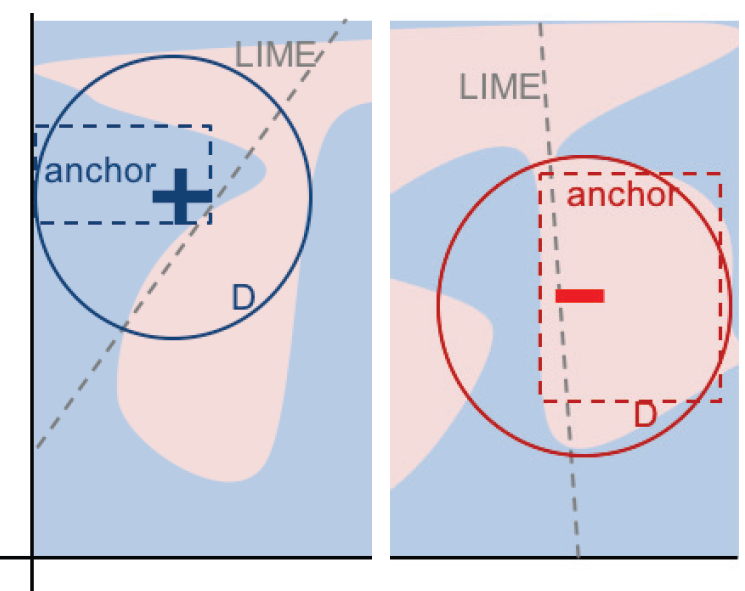
\includegraphics[scale=0.45]{pic/MA-Bilder/Literaturrecherche/Anchor.PNG}
    \caption{Funktionsweise der Anchors, entnommen aus \cite{ribeiro2018anchors}}
    \label{Fig:Funktionsweise_Anchors}
\end{figure}


%\begin{figure}[h]
%    \centering
%    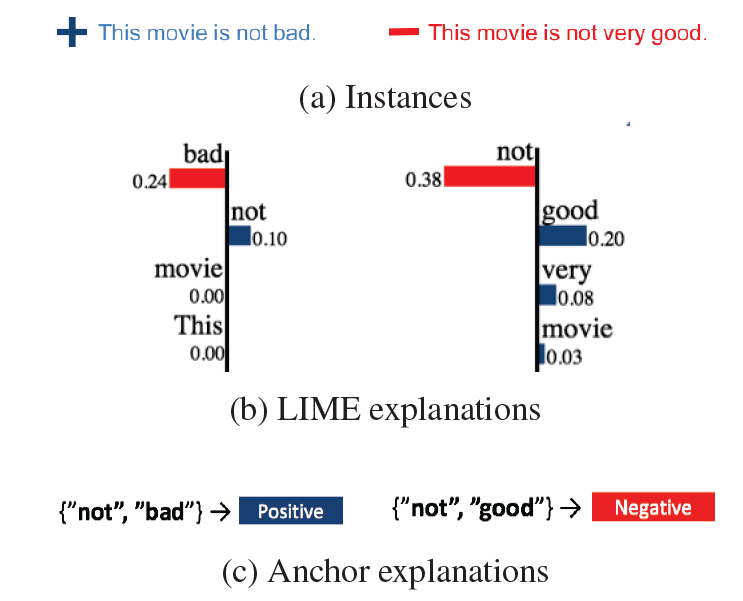
\includegraphics[scale=0.45]{pic/MA-Bilder/Literaturrecherche/Anchors-Probleme-mit-LIME.PNG}
%    \caption{Erklärungen LIME vs. Anchors, entnommen aus: \cite{ribeiro2018anchors}}
%    \label{Fig:Probleme_LIME}
%\end{figure}
%Diese Methode sollte auch eine Schwäche von LIME abdecken, welche in der Coverage (dt.: Abdeckung) besteht. Wie in \ref{subsubse_LIME} beschrieben, werden Erklärungen mittels LIME durch lokale Annäherungen an bestimmte Instanzen produziert. Was jedoch offen bleibt, ist die Frage, ob sich solche Erklärungen auch auf andere Datenpunkte übertragen lassen. Für die Nutzer eines Systems kann dies jedoch wichtig sein, um die Funktionsweise eines Systems zu verstehen und den Erklärungen vertrauen zu können, wenn genau festgelegt ist, für welche Instanzen eine Erklärung anzuwenden ist \cite{ribeiro2018anchors}. Illustriert wird dieses Problem von den Autoren selbst. So wurden sowohl mittels LIME als auch mittels Anchors Erklärungen für einen Textklassifikationsalgorithmus erstellt. Das Wort \enquote{not} ist für zwei unterschiedliche Klassenvorhersagen wichtig gewesen. Probleme können passieren, wenn Nutzer eines Systems, die Erklärung, welche mittels LIME für den Satz \enquote{The movie is not very good} auf den Satz \enquote{The movie is not bad} anwenden. Um Missverständnisse auf Nutzerseite zu vermeiden ist es wichtig, mehrere Gründe mitzugeben, die erklären, warum ein Satz welcher das Wort \enquote{not} enthält, als positiv klassifiziert wurde.

 %(\ref{Fig:Probleme_LIME}) 
 
\textbf{Formale Betrachtung}
Sei nach \textcite{ribeiro2018anchors} $f$ das Black-Box-Modell und $x$ die zu erklärende Instanz. Weiter kommt es zu einer Pertubation um $x$ herum, dessen Verteilung als $D$ definiert ist. Um einen Anchor zu definieren sei nun $A$ eine Regel, die aus einer Menge von Aussagen besteht. $A(x)$ ist dann 1, wenn alle Merkmalsaussagen wahr sind, für eine Instanz $x$. In einem Textklassifikationbeispiel, was z.B. den Satz \enquote{The Movie is not bad} als positive Aussage klassifiziert ist, $X$ der Satz und $f(x)$ positiv. Weiter wäre hier die Regel $A=\{ not, bad \}$. In Worten könnte die Regel wie folgt formuliert werden: \emph{Wenn die Wörter not und bad vorkommen, ist die Klasse positiv.} 
Sei nun $D(\cdot{}|A)$ die Verteilung von Instanzen, auf die $A$ auch zutrifft (z. B. ähnliche Texte, in denen \enquote{not} und \enquote{bad} vorkommt) \cite{ribeiro2018anchors}. $\mathcal{T}$ auf der rechten Seite der Formel gibt eine Präzisionsschwelle an. So sollen nur solche Wenn-Dann-Regeln als gültig erachtet werden, wenn sie eine lokale Treue von mindestens $\mathcal{T}$ erreichen. Formal sei also ein Anchor definiert als \cite{ribeiro2018anchors}:
\begin{equation}
    \mathds{E}_{D_{(z|A)}}[\mathbb{1}_{f(x)=f(z)}]\geq \mathcal{T}, A(x)=1
\end{equation}
\textcite{molnar2022} gibt diese Formel in eigenen Worten wieder: Wenn eine Instanz $x$ erklärt werden soll, kann dies mit einem Anchor geschehen, welcher für $x$ gilt. Hierbei sollte, die selbe Klasse für die Nachbarn von $x$ mit einer Wahrscheinlichkeit von $\mathcal{T}$ vorausgesagt werden, damit dieser Anchor anwendbar bleibt. Die Genauigkeit einer Regel ergibt sich durch das Aufrufen des Black-Box-Modells für die Nachbarn, hier notiert mit $[\mathbb{1}_{f(x)=f(z)}]$.

\textbf{Anwendung}
\textcite{ribeiro2018anchors} zeigen in ihrer Veröffentlichung die Anwendung von Anchors für Klassifikation, strukturierte Vorhersagen und Textgenerierung auf Grundlage verschiedener Datentypen (tabellarisch, textuell, visuell). Auch für das Erstellen von Anchors gibt es eine Bibliothek\footnote{https://github.com/marcotcr/anchor}, welche Entwickler unterstützt.
Für das Finden von Anchors existieren mehrere Ansätze. Ein einfacher \enquote{Bottom-Up-Ansatz} beruht darauf, mit einer leeren Regel zu starten und in Iterationen dieser Regel einen neuen Merkmalswert hinzuzufügen. Getestet würde diese Regel dann mit einer Prüfung der Genauigkeit $\mathbb{1}_{f(x)=f(z)}$  für jeden Nachbarn von $x$ \cite{ribeiro2018anchors}. Dies wäre jedoch in bei der Arbeit mit großen Datensätzen oder mit sehr vielen Merkmalsvariablen zu rechenaufwendig \cite{molnar2022}.
Daher schlagen die Autoren vor lediglich Stichproben zu ziehen und auf statistisches Vertrauen in die Genauigkeit zu setzen. Technisch geschieht die Suche, welche auch in der Anchors-Bibliothek implementiert ist mit einem Reinforcement-Learning-Ansatz (Multi-Armed-Bandit), welcher für die Modellaufrufe zuständig ist, die für das Evaluieren von Regeln sorgen. Um die besten Kandidaten für eine mögliche Wenn-Dann-Regel $A$ in die nächste Runde zu übertragen wird wird eine Balkensuche (modified Beam Search) angewendet \cite{ribeiro2018anchors}. Wie viele Kandidaten durch diese Suche begutachtet werden, bestimmt auch die geforderte Rechenleistung und die zu erreichende Genauigkeit \cite{molnar2022}
%Daher schlagen die Autoren vor den Parameter $\delta$ vor, welcher zwischen 1 und 0 liegen sollte, um eine probabilistische Definition zu erstellen. Hierdurch werden so lange Stichproben gezogen, bis statistisches Vertrauen in ihre Genauigkeit besteht. Die probabilistische Definition lautet wie folgt \cite{ribeiro2018anchors}:
%\begin{equation}
%    P(prec(A) \geq \mathcal{T}) \geq 1 - \delta  
%\end{equation}
%wobei gilt:
%\begin{equation}
%    prec(A) = \mathds{E}_{D_{(z|A)}}[\mathbb{1}_{f(x)=f(z)}]
%\end{equation}
%Weiter ist es das Ziel, die Abdeckung $cov(A) = \mathds{E}_{D_{(z|A)}}[A(z)]$ zu maximieren, also den Bereich, in der ein Anchor anzuwenden ist. Dies ist in sofern sinnvoll, als dass Regeln mit höherer Abdeckung stärker ins Gewicht fallen, da sie einen größeren Teil des Modells beschreiben. Auf der anderen Seite, sind Regeln mit einer geringeren Abdeckung präziser, sodass hier eine Abwägung zwischen Genauigkeit und Abdeckung sattfinden muss.

%Abbildung \ref{Fig:Anchors_Finden} \todo{diese Abbildung kommt wahrscheinlich noch in den Anhang} gibt einen kurzen Überblick bzgl. des Entstehungsprozesses von Anchors: 
%\begin{figure}
%    \centering
%    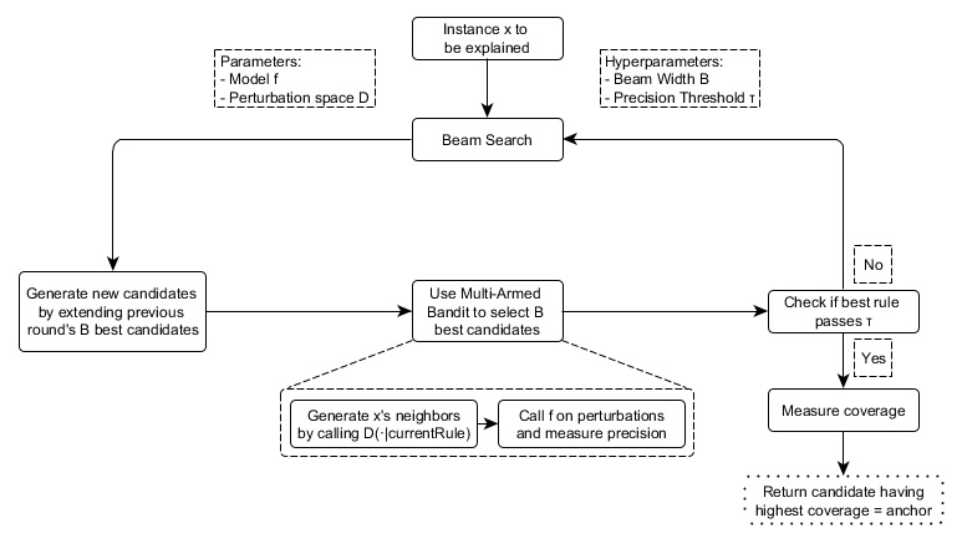
\includegraphics[scale=0.45]{pic/MA-Bilder/Literaturrecherche/Anchors_Finden.PNG}
%    \caption{Prozess zum Finden von Anchros, entnommen aus: \cite{molnar2022}}
%    \label{Fig:Anchors_Finden}
%\end{figure}

\textbf{Vor- und Nachteile}
Anchors sind einfach zu verstehen und werden dann angewendet, wenn alle Bedingungen der Regel erfüllt sind und weisen hierdurch eine hohe Genauigkeit auf \cite{ribeiro2018anchors}. Daneben können auch genaue Erklärungen entstehen, selbst wenn die lokale Nachbarschaft komplex ist. 
Anchors können sehr generell, aber gleichzeitig auch sehr spezifisch werden, was für Nutzer verwirrend sein könnte. Weiter müssen viele Modellaufrufe stattfinden, was zur Lasten der Performance geht. Weiter existiert bei der Bildklassifikation ein konzeptuelles Problem, da nicht klar ist, wie Abdeckung hier genau zu definieren ist \cite{molnar2022}.

\subsubsection{Kontrafaktische Erklärungen}
Kontrafaktische Erklärungen (engl. Counterfactual Explanations) beschreiben kausale Zusammenhänge in der Form \enquote{Wäre Merkmal A ein anderes gewesen, dann wäre auch die Vorhersage eine andere gewesen} \cite{molnar2022}. Sie bringen also Gegenargumente (engl. Counter Facts) für eine Vorhersage.

\subsubsection{Konzept}
Bisher beschriebene XAI-Methoden stellen heraus, inwiefern sich Merkmale auf eine Vorhersage auswirken. Kontrafaktische Erklärungen hingegen, beantworten die Frage, welche Änderungen an einer Eingabe vorgenommen werden müssen, um eine andere Vorhersage zu erhalten \cite{Nandi.2022}. Theoretisch wäre es zur Identifikation von kontrafaktischen Erklärungen möglich, zufällig Änderungen an der Eingabe vorzunehmen und zu beobachten, wie sich dies auf die Vorhersage auswirken würde. Zum einen ist dieses Vorgehen sehr rechenaufwendig, zum anderen hätte dies nach \textcite{molnar2022} keinen Mehrwert für Nutzer. Kontrafaktische Erklärungen lassen sich eher als eine Erklärung definieren, welche die kleinste Veränderung an der Eingabe wiedergeben, sodass sich die Vorhersage ändert. Es kann eher wünschenswert sein, dass eine kontrafaktischen Erklärung eine solche Vorhersagenerklärung ist, welche die kleinste Veränderung in den Merkmalswerten wiedergibt, was zu einer Änderungen in der Vorhersage führt. Eine Herausforderung, die diese Erklärungen meistern müssen, basiert auf dem sogenannten Rashomon-Effekt. Rashomon ist ein Film, in dem Akteure eine Geschichte aus unterschiedlichen Perspektiven erzählen. Jede einzelne Geschichte ist in sich schlüssig, jedoch widersprechen sie sich untereinander. Dieses Phänomen kann auch bei kontrafaktischen Erklärungen auftreten. So könnte eine Erlkärung verlangen den Wert $x_1$ zu ändern, während eine andere vorschlägt Merkmal $x_2$ zu modifizieren, es können also mehrere gültige kontrafaktische Erklärungen existieren. Es Um Anforderungen an die kontrafaktischen Erklärungen zu definieren ist es wichtig, dass Nutzer definieren, was genau eine relevante Veränderung in der Vorhersage einer Instanz ist (z.B. Genauigkeit oder andere Klasse). 
%Jedoch ist es nicht immer möglich, eine kontrafaktische Erklärung zu erstellen, welche den Nutzerwünschen gut entspricht. Als Beispiel sei hier genannt, dass es eine Klassifikation mit nur zwei Klassen gibt, die jedoch unausgeglichen verteilt sind. So liegen in der einen Klasse sehr viele und in der anderen sehr wenig Datenpunkte. So würde sich die Vorhersage zur weniger repräsentativen Klasse nur sehr schlecht ändern lassen (oder man müsste sehr viele Merkmale ändern). Hier sollte sich ein Nutzer dann dazu entscheiden, nicht die Klasse selbst, sondern die Genauigkeit der Vorhersage ändern zu wollen.
Daneben ist es in der Realität sinnvoll, solche Erklärungen zu geneieren, die ungefähr dem Original entsprechen. Bei einen Algorithmus, welcher bspw. die Preise für eine Wohnung vorhersagt, sollte die Quadratmeter-Zahl der Wohnung nicht negativ werden \cite{molnar2022}.

\textbf{Formale Grundlagen}
Für eine zu erklärende Instanz $x$ muss ein Kontrafakt $x'$ gefunden werden \cite{kamath2021explainable}. Für dieses $x'$ sollte das zugrundeliegende Modell $f$ die eine andere Vorhersage als für $x$ ausgeben, hier mit $y'$ notiert. Wie vorangegangen beschrieben, besteht weiter das Ziel, dass sich das Kontrafakt nicht besonders von der zu betrachtenden Instanz unterscheidet (hier durch $d$ angegeben). Dies lässt sich formal in folgendem Optimierungsproblem $L$ beschreiben\cite{kamath2021explainable}:
\begin{equation}
    \underset{x'}{min} \: L(x'|x) = (f(x')-y')^2 + \lambda d(x, x')
\end{equation}
$\lambda$ bestimmt das Verhältnis von $(f(x')-y')^2$ und der Distanzfunktion $d$. Für einen großes $\lambda$ wird ein Kontrafakt erstellt, welches sich in den Merkmalswerten von $x$ wenig unterscheidet. Für einen kleinen Wert werden solche Kontrafakte erstellt, die sich sehr nahe an der gewünschten Ausgabe $y'$ befinden. Das Kontrafakt $x'$ und dessen Merkmalswerte können nun genutzt werden, um mit Bezug auf die ursprüngliche Instanz eine Wenn-Dann-Regel aufzustellen, die beschreibt, welche Werte für eine andere Vorhersage geändert werden müsste.


%Für das Generieren dieser Erklärungen existieren unterschiedliche Möglichkeiten. Eine wurde von \textcite{wachter2017counterfactual} vorgestellt. Hier sind $w$ die Gewichte, $f$ ist der ML-Algorithmus, $yi$ ist die Zielvariable, $xi$ ist ein Datenpunkt. Gesucht ist nun ein Kontrafakt ($x'$), welches sich in der Nähe von $xi$ befindet, aber $fw(x)$ soll der von den Nutzern definierten Zielvariable $yi$ entsprechen. Nach \textcite{wachter2017counterfactual} ließe sich dies realisieren, indem folgende Gleichung minimiert wird, während $w$ nicht verändert wird: 
%\begin{equation}
%    arg \: \underset{x'}{min} \: \underset{\lambda}{max} \: \lambda (f_{w}(x') - y')^{2} + d(x_{i}, x')
%\end{equation}

%$d$ ist hier eine Funktion, welche berechnet, wie weit das Kontrafakt vom ursprünglichen Punkt $x$ entfernt ist. In Realität wird $\lambda$ maximiert, indem iterativ $x'$ gefunden wird und $\lambda$ erhöht wird \cite{wachter2017counterfactual}. Nach \cite{wachter2017counterfactual} kann für dieses Problem jeder Optimizer verwendet werden, 

\textbf{Anwendung}
Für kontrafaktische Ekärungen bestehen sowohl modell-agnostische (\cite{dhurandhar2019model, guidotti2018local}) als auch modellspezifische Ansätze (\textcite{wachter2017counterfactual, mothilal2020explaining}), welche sich z.B. die Gewichte von neuronalen Netzen zu Nutze machen. Die DICE-Bibliothek von Microsoft bietet Möglichkeiten zur Generierung von kontrafaktischen Erklärungen an \footnote{https://www.microsoft.com/en-us/research/project/dice/}. Beim Benutzen dieser Biblothek kann angegeben werden, wie viele kontrafaktische Erklärungen produziert werden soll.

\textbf{Vor- und Nachteile}
Ein Vorteil, welchen kontrafaktische Erklärungen gegenüber anderen Methoden wie z.B. LIME besitzen, ist ihre Genauigkeit. Sie stellen relativ klar heraus, welche Merkmale geändert werden müssen. LIME z.B. kann keine Aussagen über den genauen Wert geben, da diese nur lokale Genauigkeit besitzen, wie in Abbilung \ref{Fig:Lime-Funktionsweise} gezeigt. Daneben sind sie für Menschen gut verständlich \cite{molnar2022}. Ein Nachteil dieser XAI-Methode besteht in dem grundsätzlichen Rashomon-Effekt, der es erschwert, die richtige Erklärung auszuwählen \cite{kamath2021explainable}. Im Zweifel sollten den Nutzer daher eine größere Zahl vieler verschiedener Erklärungen präsentiert werden \cite{molnar2022}. Daneben haben einige Methoden, z.B. die von \cite{wachter2017counterfactual} zum Finden der Kontrafakte, dass Problem, nicht nur solche Kontrafakte zu finden, welche wenig Merkmale abändern. Des Weiteren werden auch unrealistische Merkmale miteinbezogen \cite{molnar2022}
%Dies wird von einer anderen Methode jedoch erfüllt (\cite{dandl2020multi}).


\subsection{Modellagnostische Methoden - global}
\subsubsection{Partial Dependence Plot}
\label{subsubsec_PDP}
Ein Partial Dependence Plot kann zur Visualisierung eingesetzt werden, nachdem ein Modell trainiert wurde \cite{Gianfagna.2021}. Sie verfolgt das Ziel aufzudecken, inwiefern Merkmale die Black-Box-Modell-Ausgaben beeinflussen. Diese Art der Darstellung misst, wie sich ein Merkmal auswirkt, wenn man den Wert diesen immer etwas abändert, aber die Werte der anderen Merkmale nicht modifiziert. \cite{kamath2021explainable}.
Vereinfacht gesagt würde man bei zwei Variablen, die jeweils z.B. einen möglichen Wert von 1-5 annehmen können, für das erste Merkmal das Modell mit dem Wert 0 aufrufen, während man das zweite Merkmal nicht verändert. Im nächsten Schritt würde man den Wert des ersten Merkmals auf 1 setzen usw. Ist dies für alle möglichen Werte des ersten Merkmals geschehen, wird der Mittelwert der Vorhersagen berechnet. Dies wird daraufhin für das zweite Merkmal wiederholt. 
Formal ist die PD definiert mit $d$ als Anzahl der Merkmalen (\cite{kamath2021explainable} nach \cite{friedman2001greedy}): 
\begin{equation}
    PD(x_{1}) = \mathds{E}_{x_{2}}[f(x_{1},x_{2})] = \int p(x_{2}) f(x_{1},x_{2})d_{x_{2}}
\end{equation}
Abbildung \ref{Fig:PDP_Beispiel} zeigt ein Beispiel für einen PDP. 
\begin{figure}[h]
    \centering
    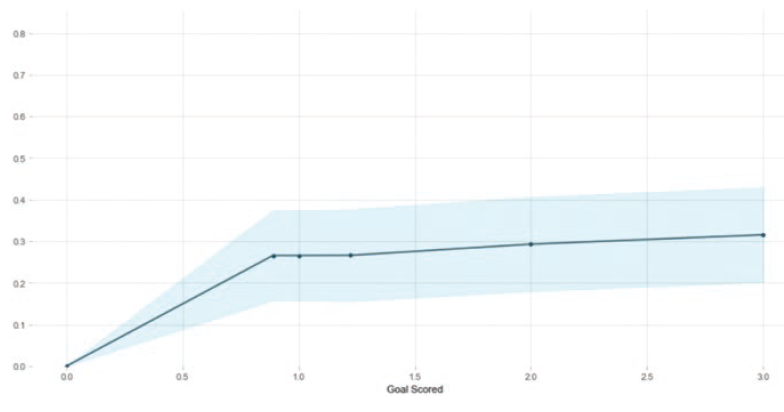
\includegraphics[scale=0.45]{pic/MA-Bilder/Literaturrecherche/PDP-Beispiel.PNG}
    \caption{Beispiel für einen PDP, entnommen aus: \cite{Gianfagna.2021}}
    \label{Fig:PDP_Beispiel}
\end{figure}

%Für die Anwendung eines PDP existiert ein Modul von Scikit-Learn \footnote{https://scikit-learn.org/stable/modules/partial_dependence.html}
%Hiermit schaut man, welche Effekte Features auf den Output haben \cite{kamath2021explainable}, dies ist eine glibale Methode und zeigt Beziehungen zwischen den merkmalen in den Input und den Vorhersagen auf. PD-Diagramme visualisieren die partielle Abhängigkeitsfunktion, die die Wirkung eines Merkmals durch Abgrenzung über andere Merkmale misst. Bei einem Modell mit zwei Merkmalen, f (x1, x2), wird die partielle Abhängigkeitsfunktion des Merkmals x1 beispielsweise durch Mittelung über die Randverteilung des Merkmals x2

Ein Vorteil der PDP-Methode ist es weniger zu zeigen, welches Merkmal den größten Einfluss auf eine Vorhersage hat (wie z.B. die Methode der Permutation Importance \todo{dazu muss ich noch ein Kapitel schreiben}), sondern bestimmte Schwellenwerte aufzudecken. So können PDP dabei helfen, zu definieren, wie ein Wert eines Merkmals besetzt sein sollte, um ein bestimmtes Ergebnis zu bekommen \cite{Gianfagna.2021}. 
%Youtube-Video(https://www.youtube.com/watch?v=uQQa3wQgG_s):
%Man hat die Datensätze mit den Features, Beispiel: alle Features haben Werte von 0-5 oder so, dann setzt man von EINEM Feature alle diese Werte von dem Feature auf 0 --> dann berechnet man (mit den anderen Features zusammen),was jeweils raus kommt (Rest der Daten bleibt gleich) --> dann hat man ganz viele Vorhersagen und nimmt dann die Average von den ganzen --> dann wei0 man, wie das die Vorhersage beeinflusst, wenn der Wert des Features 0 war --> dann setzt man das auf 1 und berechnet die Average und so weiter
%dann plottet man das und sieht halt --> Average Vorhersage, wenn Feature 0,1,2,3,4,5 war
%Das macht man halt mit allen Features
Ein Nachteil dieser Methode beruht auf der Annahme, dass die Merkmale unabhängig voneinander sind. So wird, wie oben erklärt, der Wert des ersten Features nach Belieben geändert, während der Wert des zweiten Features gleich bleibt. Jedoch führt dies zu Kombinationen, welche in der Realität nicht vorkommen können \cite{molnar2022}.
%Youtube-Video:
%Nachteil der Average-Funktion: starke Vereinfachung, wäre cool zu sehen, ob die verschiednene Predicted Values sehr stark aneinander liegen oder eben nciht (man könnte Verteilung darstellen, anstatt nur die Punkte)
%Hier Beispiel einfügen: 

Eine weitere ähnliche Methode ist der \emph{Accumulated Local Effects (ALE) Plot} nach \textcite{apley2020visualizing}, welches das Problem der Abhängigkeit löst.
%TODO das vlt. noch machen, gutes, aber langes Video hier: https://www.youtube.com/watch?v=06knUxoig9Y

\subsubsection{Individual Conditional Expectation (ICE)}
\begin{figure}[h]
    \centering
    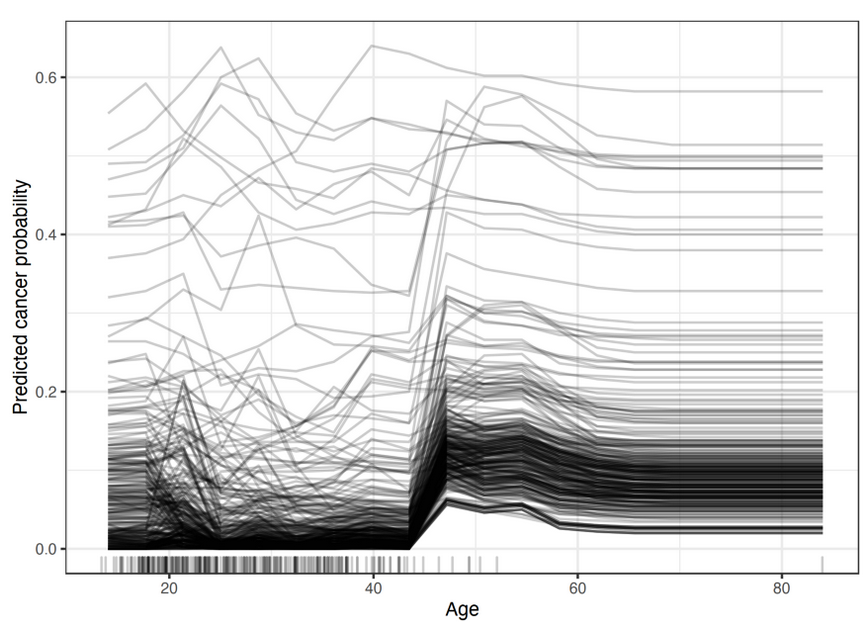
\includegraphics[scale=0.35]{pic/MA-Bilder/Literaturrecherche/ICE_Beispiel.PNG}
    \caption{Beispiel für ICE, entnommen aus: \cite{ICE-beispiel}}
    \label{Fig:Beispiel_ICE}
\end{figure}
Die Funktionsweise der ICE-Methode ist die selbe der PDP (vgl. Unterkapitel \ref{subsubsec_PDP}), wir hier jedoch lokal anstatt global angewendet, indem die Werte für jede Instanz berechnet werden \cite{molnar2022}. Somit lassen sich der Einfluss von Änderungen einzelner Features bestimmen \cite{hanif2021survey}. Nach \textcite{molnar2022} ist ein PDP ein Mittelwert der ICE. ICE kann jedoch eine gute Alternative bieten, tiefere Einblicke in die Feature-Interaktionen zu erhalten \cite{molnar2022}. In Abbildung \ref{Fig:Beispiel_ICE} ist ein Beispiel für eine ICE zu sehen: 

\subsubsection{Global Surrogate}
Um jedes beliebige Black-Box-Modell zu erklären, kann ein interpretierbares Modell eingesetzt werden, welches sich dem ursprünglichen Modell annähert. Diese Methode heißt Global Surroagte (globaler Stellvertreter) \cite{molnar2022}. In Kapitel \ref{subsubse_LIME} ist dieses Konzept lokal beschrieben. Ziel dieser Methode ist eine ungefähre Abschätzung des ursprünglichen Modells, während Interpretierbarkeit gewährleistet wird. Entscheidend bei dieser Methode ist die Wahl des Modells, denn dieses muss interpretierbar sein. Eine Auswahl von transparenten Modellen ist in Kapitel \ref{subsubsec_transparenteModelle} zu finden, so sind bspw. lineare Modelle oder Entscheidungsbäume geeignet \cite{molnar2022}.

Die Implementation eines solchen globalen Stellvertretermodells ist relativ simpel, so wird kein Zugriff und auch kein Wissen über die Modellstruktur benötigt. Entwickler, welche einen globalen Stellvertreter entwickeln wollen, müssen sich zunächst für einen Datensatz entscheiden und für diesen die Vorhersagen abrufen. Im nächsten Schritt wird sich für ein interpretierbares Modell entschieden, welches dann auf die ursprünglichen Daten und Vorhersagen trainiert wird. Daraufhin findet eine Evaluation statt \cite{molnar2022}.

Eine Möglichkeit, zu überprüfen, wie exakt der Stellvertreter das Black-Box-Modell annähert, ist das $R^{2}$-Maß, welches wie folgt definiert ist:
%SSE ist Summe von Squares Error und SST ist Summe of Squares Gesamt (1-\frac{SSE}{SST}=)
\begin{equation}
    1-\frac{\sum_{i=1}^n(\hat{y}_{*}^{(i)}-\hat{y}^{(i)})^{2}}{\sum_{i=1}^n(\hat{y}^{(i)}-\bar{\hat{y}})^{2}}
\end{equation}

Die Vorhersage des interpretierbaren Modells ist für die i-te Instanz $\hat{y}_{*}^{(i)}$, während die Vorhersage des Urpsrungmodells mit $\hat{y}^{(i)}$ notiert ist. $\bar{\hat{y}}$ gibt den Mittelwert der Vorhersagen des Black-Box-Modells an. Wenn sich das Ergebnis in der Nähe von 1 befindet, ist dies so zu verstehen, dass der Stellvertreter sich dem Modell gut annähert. Nähert sich der Stellvertreter sehr gut an, kann sogar in Betracht gezogen werden, dieses anstatt des ursprünglichen Modells zu verwenden. Liegt der Wert nahe bei 0, bedeutet dies analog, dass sich das Stellvertretermodell nicht eignet \cite{molnar2022}. %R sagt nix über die Performance des Black-Box-Modells aus, sondern nur wie gut der Stellvertreter das immitiert.

Ein Vorteil dieser Methode ist dessen einfache Anwendung. Daneben kann flexibel jedes mögliche Modell als Stellvertreter gewählt werden. So kann sowohl auf die Kenntnisse der Entwickler als auch auf die der Nutzer eingegangen werden. Wenn alle Stakeholder sich z.B. gut mit Entscheidungsbäumen auskennen, kann dieses Modell als Stellvertreter gewählt werden. Daneben existieren natürlich auch Nachteile dieser Methode. Jedes interpretierbare Modell bringt selbst seine eigenen Schwächen mit und es werden Annahmen über das Black-Box-Modell getroffen, welche eventuell nicht der Wahrheit entsprechen. Dazu kann es eine schwierige Entscheidung sein, welcher $R^{2}$-Wert als ausreichend betrachtet wird.

\subsubsection{Protoypen und Kritiken}
XAI-Modelle können auch mit konkreten Dateninstanzen erklärt werden. Als Protoypen werden solche Instanzen bezeichnet, die einen Datensatz repräsentieren, während Kritiker solche Datenpunkte sind, welche schlecht die gesamten Datensätzen wiedergeben. %(https://christophm.github.io/interpretable-ml-book/proto.html#proto)
Mit diesen Konzepten lassen sich sowohl Datensätze als auch ML-Modelle erklären, was in Abbildung \ref{Fig:Prototyp_Kritiekr} dargestellt ist für Instanzen, welche die Merkmale $x1$ und $x2$ in unterschiedlicher Ausprägung besitzen \cite{molnar2022}.
\begin{figure}
    \centering
    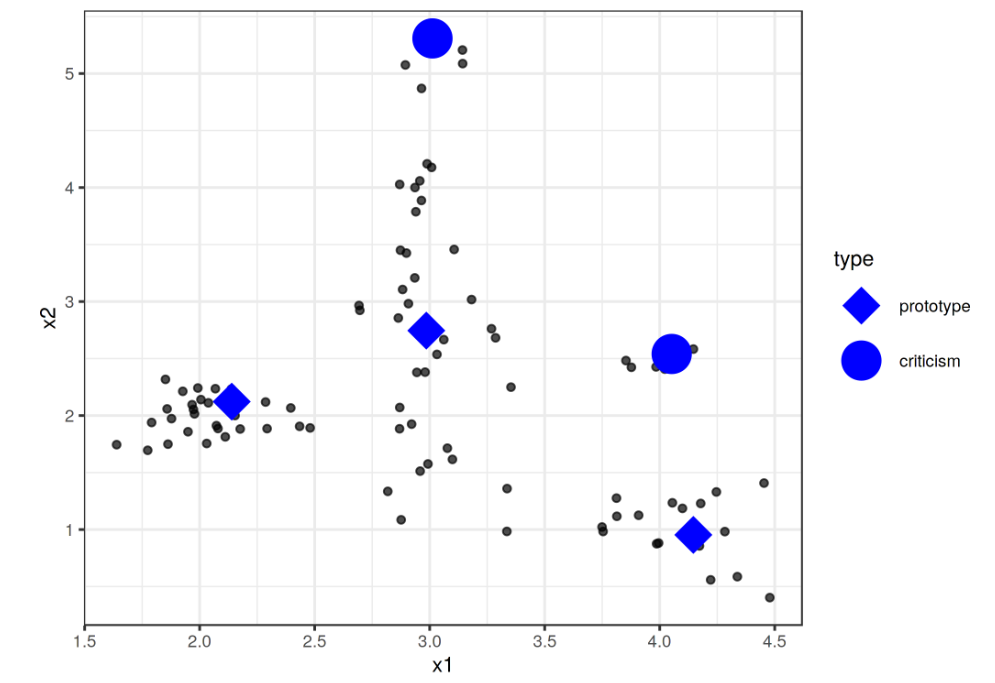
\includegraphics[scale=0.45]{pic/MA-Bilder/Literaturrecherche/Prototyp_Kritiker-Beispiel.PNG}
    \caption{Protoypen und Kritker, entnommen aus: \cite{molnar2022}}
    \label{Fig:Prototyp_Kritiekr}
\end{figure}
Zum Finden dieser Datenpunkte existieren verschiedene Methode. Die einfachste Methode stammt von \textcite{rdusseeun1987clustering}, lässt sich jedoch nur für Protoypen anwenden. Diese Methode heißt \emph{k-medoids} und funktioniert ähnlich zu der in Kapitel \ref{subsubsec:k-means-Clustering} beschriebenen Methode k-means Clustering. Eine weitere Methode, die sowohl das Identifzieren von Protoypen als auch Kritiker ermöglicht, heißt \emph{MMD-critic} und wurde von \textcite{kim2016examples} vorgestellt. % Das kann man auch direkt benutzen: %https://github.com/BeenKim/MMD-critic und hier: Recently an extension of MMD-critic was developed: Protodash. The authors claim advantages over MMD-critic in their publication. A Protodash implementation is available in the IBM AIX360 tool.
\todo[inline]{Hier kommt noch eine Beschreibung der MMD-Critic-Methode}
\subsection{Modellspezifisch: Neuronale Netze}
Folgendes Unterkapitel beschäftigt sich mit solchen Methoden, welche sich auf neuronale Netze anwenden lassen.
\subsubsection{Layer-wise Relevance Propagation}
Layer-wise Relevance Propagation (LRP) wurde erstmals von \cite{bach2015pixel} vorgestellt und zeigt bei neuronalen Netzen die Relevanz eines Eingabewertes für die Ausgabe. \textcite{bach2015pixel} illustrieren dies in ihrem Paper sehr gut anhand eines Klassifikationsalgorithmus (CNN), welcher Bildern eine Klasse zuweist. Ein bestimmter Pixel ist hier die Eingabe und ist auf eine gewisse Weise für die Vorhersage verantwortlich. Um herauszufinden welche Pixel eines Bildes sich besonders auf die Vorhersage auswirken, wir im Rahmen der LRP-Methode ein Relevanzwert für jedes Neuron in jedem Layer berechnet, indem rückwärts durch das neuronale Netz gegangen wird. Somit wird sich in verkehrter Reihenfolge dem Input angenähert und die relevanten Pixel werden sichtbar. Dies nennen die Autoren \enquote{pixel-wise decomposition} \cite{bach2015pixel}. \textcite{bach2015pixel} stellen folgende Möglichkeit zur Berechnung der Relevanzwerte vor:
%Wie berechnet man nun die Scores? Man hat nun R14(erstes(und gleichzeitig einziges) Neuron im vierten (letzten) Layer), das hat z.B. einen Score von 0,8, dass es eine Katze ist - das ist unser erster Relevanz-Wert. Die Relevanz rechnet man nun so aus (Beweis siehe Orignalpaper): Relevanz ist R für das Neuron i, l ist der Layer:
\begin{equation}
    R_{i}^{(l)} = \sum_{i} \frac{z_{ij}}{\sum_{i'}z_{i'j}}R_{j}^{l+1} \text{wobei gilt:}\: z_{ij}=x_{i}^{(l)}w_{ij}^{(l,l+1)}
\end{equation}
$l+1$ sei hier der letzte Layer, mit dem gestartet wird und somit wird von hinten für jedes Neuron $j$ im Layer $l+1$ die Aktivierung berechnet. Diese Aktivierung ergibt sich dadurch, inwiefern sich ein Neuron $i$ im Vergleich zu den anderen Neuronen in dem Layer $l$ auswirkt. So werden die Gewichte mit dem Input $x$ mutlipliziert, welche sich jeweils in den nächsten Layer übertragen. Die Aktivierung gibt Aufschluss darüber, wie relevant ein Neuron jeweils für den nachfolgenden Layer (und somit auf den endgültigen Output) war. Ist dies für alle Layer geschehen, wird der ursprüngliche Input, also die Pixel des Bildes erreicht. Diese lassen sich dann visualisieren.

%Für die Anwendung von LRP kann eine Bibliothek unterstützen %\footnote{https://github.com/sebastian-lapuschkin/lrp_toolbox}.
\subsubsection{Saliency Maps}
Saliency Maps basieren auf einem ähnlichen Prinzip wie die LRP-Methode und lassen sich auch auf Bildklassifikation anwenden. Hier wird auch gezeigt, welche Teile eines Bildes releavant für die Vorhersage waren und es wird auf die innere Struktur des Netzwerkes zurückgegriffen \cite{Gianfagna.2021}.
Saliency Maps wurden zuerst vorgestellt von \cite{simonyan2013deep} und basieren auf der Berechnung, der Gradienten, welche bei der Optimierung der Verlustfunktion von neuronalen Netzen zum Einsatz kommen. Konkret helfen Gradienten dabei die Verlustfunktionsparameter zu optimieren, in dem vorgegeben wird, wie weit sich auf einer Funktion bewegt werden muss \cite{molnar2022}.

Nach \textcite{simonyan2013deep} gibt es hier ein Bild $I_{0}$ und eine Klasse $c$. Daneben existiert eine Klass-Score-Funktion $S_{c}(I)$. Ziel ist es, die Pixel anhand ihres Einflusses auf den Score $S_{c}(I)$ zu ordnen. Dieser Score ist zumeist in CNNs nicht linerar berechenbar, lässt sich jedoch annähern (mithilfe einer Taylor Series Expansion):
\begin{equation}
    S_{c}(I) \approx w^{T}I+b
\end{equation}
Analog zum Grundlagenkapitel sei hier b der Bias und $W$ sind die Gewichte. Die Saliency Map lässt sich für ein Merkmal $j$ wie folgt bestimmen \cite{kamath2021explainable}: 
\begin{equation}
    M_{j} = |w_{j}|
\end{equation}

Ein Beispiel für eine Saliency Map ist in Abbildung \ref{Fig:Saliency_Map_Beispiel} dargestellt.
Ein Vorteil dieser XAI-Methode besteht in ihrer leichten Berechnung und dass keine weiteren Annotationen zur Erklärung eingeführt werden müssen \cite{kamath2021explainable}. \textcite{Gianfagna.2021} schreiben jedoch, dass diese Art der Darstellung für Menschen nicht besonders hilfreich ist, da wenig erkannt werden kann. Daneben besteht ein Nachteil, welcher sich durch die Score-Funktion ergibt. Ist diese nicht ableitbar, lässt sich kein geeigneter Score ermitteln, was z.B. für die ReLu-Funktion gilt \cite{shrikumar2017learning}. DeconvNet von \cite{zeiler2014visualizing} ist ein ähnlicher Ansatz, welcher das Problem mit der ReLU-Function löst. Grundsätzlich können jedoch auch LIME oder SHAP für das Erstellen von Saliency-Maps genutzt werden \cite{molnar2022}.
\begin{figure}[h]
    \centering
    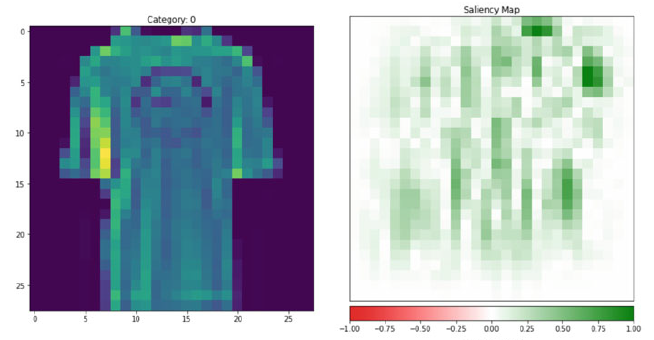
\includegraphics[scale=0.45]{pic/MA-Bilder/Literaturrecherche/Saliency-Map-Beispiel.PNG}
    \caption{Beispiel für Saliency Map, entnommen aus: \cite{kamath2021explainable}}
    \label{Fig:Saliency_Map_Beispiel}
\end{figure}

\subsubsection{TCAV}
TCAV steht für \enquote{Testing with Concept Activation Vectors} und wurde von \textcite{kim2018interpretability} vorgestellt. Diese Methode konzentriert sich darauf, mithilfe von Konzepten die Funktionsweise von neuronalen Netzen Menschen näher zu bringen. Nach \textcite{kim2018interpretability} bringen viele andere XAI-Methoden den Nachteil mit sich, dass die Fokussierung auf Merkmale schlecht für Nutzer zu interpretieren ist. Merkmale liegen häufig in niedriger Abstraktionsebene vor, aber Menschen denken nicht auf niedriger, sondern auf hoher Abstraktionsebene - in Konzepten. 
%Motiviert wird die TCAV-Methode durch eine Schwäche von Saliency Maps und den sogenannten \enquote{Confirmation Bias}. Sie untersuchten verschiedene Arten von Saliency Maps und fanden heraus, dass selbst, nachdem sie das Modell so modifizierten, dass dieses zufällige Vorhersagen traf, die Maps sich kaum veränderten. %Hier kommt der \enquote{Confirmation Bias} ins Spiel. Wenn Menschen etwas bestimmtes erwarten, z.B. das ein Bild einer Katze so erklärt wird, dass die Umrisse von Katzenohren hervorgehoben werden, vertrauen sie dieser Erklärung durch eine Saliency Map, selbst dann, wenn dies nicht durch das Modell erkannt wird. 
%Ein Problem kann sein, dass Pixel genutzt wurden und nciht high-Level (Menschen denken nciht in Pixel)
%Sie wollen high-Level-Konzepte nutzen. Sie sieht Interpretierbarkeit als Optimisierungsproblem, man muss eine Erklärung E finden, so dass Q maximiert ist. Das Q kann eine subjektive Measures sein, sodas man Menschen fragt, aber auch 
%\begin{equation}
%    \underset{E}{argmax} Q(E|?)
%\end{equation}

%Sie sagt auch ncoh, wie man das gut prüfen kann, ob eine Erklärung gut war: gib Menschen Task, für die Verständnis über das Modell wichtig ist --> wenn die die gut können, bedeutet dass, dass sie das Modell verstanden haben

%kommt nur im Youtube-Video vor:
%Modell Matters--> also linear ist einfacher als krumme komische Geraden
%Data Matters --> wenn die Daten voll gut linear abtrennbar sind, weil sie so sind, ist es einfach, aber wenn die überall drin liegen und die lineare Gerade dadurch sich nur annähert, ist doof, Daten sind halt nicht so
%Empfänger matters: wenn ich es Nutzern erläre oder Leuten, die es weiterentwickeln wollen, stellen die andere fragen
%Task matters: lokal vs. global, eibfach vs. komplex (dafür genauer), Domäne (einfach oder leicht)
 
%TCVA: ist eine Post-Methode
Die TCVA-Methode kann genutzt werden, um auf hoher Abstraktionsebene zu testen, ob ein bestimmtes Konzept in die Vorhersage des Algorithmus miteinfloss. Dies ist sogar dann möglich, wenn dieses Konzept nicht Teil des Trainingsdatensatzes war. Illustriert wird die Fuktionweise in Abbildung \ref{Fig:TCAV} \cite{kim2018interpretability}.

\begin{figure}[h]
    \centering
    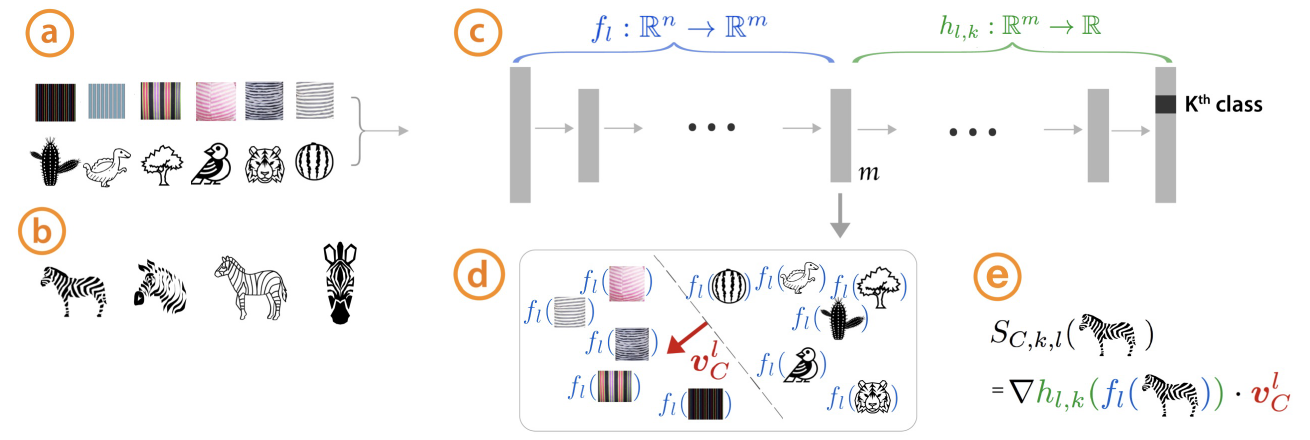
\includegraphics[scale=0.45]{pic/MA-Bilder/Literaturrecherche/TCAV.PNG}
    \caption{Funktionsweise von TCAV, entnommen aus: \cite{kim2018interpretability}}
    \label{Fig:TCAV}
\end{figure}
Als Beispiel ist hier ein neuronales Netz, welches Bilder klassifziert und ausgibt, ob sich auf dem Bild ein Zebra befand. Was nun von Interesse sein kann, ist die Frage, ob das Konzept \emph{Streifen} mit in die Bestimmung der Vorhersage einfloss. Konzepte lassen sich als Vektoren (CVA: Contept Activation Vector) definieren. Um einen solchen Vektor zu bilden, sind zunächst Beispiele von Nöten, z.B. Bilder von Streifen. Daneben werden noch andere, zufällige Bilder benötigt. Eine weitere Voraussetzung für das Durchführen der TCAV-Methode ist der Zugang zum Netzwerk und seinen Aktivierungen. Zu Beginn werden alle Beispiele (solche mit Streifen und solche ohne) durch das Netzwerk geleitet und die Aktivierungen gesammelt. Daraufhin wird ein linearer Klassifikationsalgorithmus trainiert, welcher die beiden Klassen voneinander abgrenzt. Der CVA steht nun orthogonal auf der durch den linearen Klassifzierungsalgorithmus erstellten Entscheidungsgrenze und zeigt auf die Bilder, welche Streifen enthielten. Nun kann mittels des Vektors das Konzept getestet werden.
\todo{Hier fehlt noch, wie das Testen an sich funktioniert}

%Man betrachtet Konzept zu CAV: Man nimmt jetzt das Konzept (den Vektor) und das Bild (das Zebra) und verändert das Bild so, dass man mehr oder weniger von dem Konzept nimmt und schaut, ob siech die Prediciton-Wahrscheinlichkeit für Klasse Zebra verändert. Wenn es sich gar nicht verändert, ist das Konzept nicht wichtig
%Man nimmt jetzt viele Zebra-Bilder und schaut wieviele positiv directional für CAV(Streifen) ausgaben

%Problem mit den Images, einige waren random und daher fragt sich KIM: Hat mein CAV nur hohe Empfindlichkeit durch Zufall geliefert? --> das kann man überprüfen, indem man ganz viele Random Images merhmals mit den Streifen vergleicht und hierfür mehrer TCAVs macht %todo weglassen oder verstehen :D
%Wenn das Konzept wirklich sinnvoll ist, dann der TCAV-Score auch immer ähnlich sein
%Vorteil: Nutzer kann mit eigenen Konzepten ankommen und braucht nix über ML zu wissen

%\cite{molnar2022}Methode kann globale erklärungen über Konzepte liefern
%\cite{kim2018interpretability} haben Methode vor allem auf Bildern angewendet, und es ist halt schwierig die Konzepte automatisch zu identifzieren, dafür braucht es halt Menschen

\todo[inline]{Ich würde noch die zwei unvollständigen Kapitel fertig schreiben und dann noch die Methode DeepLift, Neural Shrubs und etwas zu Feature Interaktionen schreiben}
\subsection{Weitere Methoden}
\todo[inline]{Wenn das in Ordnung ist, würde ich hier noch einige Methoden auf hoher Abstraktionsebene beschreiben. Es gibt halt sehr viele, und ich glaube nicht dass ich jede (und schon gar nicht zu genau) beschreibene sollt. In der folgenden Auflistung siehst du ein paar von den Methoden, welche mir theoretisch fehlen würde, auch wenn dies nicht alle sind, die ich insgesamt gefunden habe.}
\begin{itemize}
    \item CAM with global average pooling (Sonderformen: Grad-CAM, Guided Grad-CAM mit Feature Occlusion, Repsond CAM, Multi Layer CAM)
    \item DeepLIFT
    \item Prediction Difference Analysis 
    \item Slot Activation Vectors
    \item PRM (Peak Response Mapping)
    \item direct output labels
    \item Image Corruption and Testing Region of interest
    \item Attention map with autofocus convolutional layer
    \item DecnovNet
    \item SVD
    \item CCA
    \item SVCCA
    \item DWT
    \item Explanation Vector
    \item LSTMVis
\end{itemize}

\todo[inline]{Die Methoden könnten dann so oder so ähnlich beschrieben werden}
\textbf{PCA}
\begin{addmargin}[25pt]{0pt}
Principal Component Analysis wurde von \cite{pearson1901liii} eingeführt. und kann zur Feature Extraktion genutzt werden \cite{tjoa2020survey}. Hier wird weniger ein Modell erklärt, als dass die Dimensionen der jeweiligen Merkmale reduziert werden und somit für den Nutzer einfacher verständlich werden. %(https://medium.com/apprentice-journal/pca-application-in-machine-learning-4827c07a61db)
\end{addmargin}

\subsection{Präsentation von Erklärungen}
Neben dem Erstellen der Erklärung, existieren auch einige Hinweise in der wissenschaftlichen Literatur, wie diese an den Erklärungsempfänger zu übermitteln sind.
\subsubsection{Integration von Domänenwissen und Kontext}
Nach \cite{zhou20182d} ist die Integration von Domänenwissen besonders wichtig, um Erklärungen verständlicher und praxisorientierter zu gestalten. \cite{sun2005explanation} integrierten bspw. Domänenwissen in bayesche Netzwerke.

\subsubsection{Form der Präsentation}
\cite{weitz2019you} überprüfen in ihrer Veröffentlichung, ob ein virtueller Agent die von dem XAI-Algorithmus erstellten Erklärungen an Endnutzer kommunizieren könnte. Ergebnis dieser Untersuchung, dass menschliche Züge eines virtuellen Agenten die Interaktion erleichtern, was gleichzeitig zu einem besseren Verständnis und auch zu mehr Vertrauen auf Endnutzerseite führt. Hier sei jedoch angemerkt, dass Vertrauen schwer zu messen ist \cite{weitz2019you}.  Auch \cite{vaughan2020human} stellen heraus, dass für Menschen verbale sowie nonverbale Kommunikation zum Verständnis hilfreich ist.
Um für Menschen verständlichere Erklärungen generieren zu können, haben \cite{kim2020answering} eine Methode entwickelt, welche aus Charts (z.B. Balkendiagrammen) automatisch einen beschreibenden Text generieren kann.

\subsubsection{Interaktivität}
Bei der Präsentation können Visualisierungstools helfen. Interaktivität ist ein besonders wichtiges Element dieser Tools, da ein Vor- und Zurückgehen durch die Daten und Erklärungen hilfreich sein können, um die Daten und die Funktionsweise des Modells besser zu verstehen. Des Weiteren kann der Nutzer sich selbst aussuchen, was für sein Verständnis wichtig ist und wie er Informationen am besten aufnimmt \cite{vaughan2020human}. Es existieren auch Untersuchungen im wissenschaftlichen Kontext, welche die Vorteile von Interaktivität untersuchten. So fanden \cite{vaccaro2018illusion} heraus, dass Menschen mit dem Output eines System zufriedener sind, wenn sie diesen mithilfe von einem interaktiven Schieberegler abfragten. Außerdem hilft Interaktivität und die Möglichkeiten des Nutzers den Output der XAI-Methoden mitzubestimmen, dabei explorative Experimente durchzuführen \cite{weld2019challenge}. Dies erlauben beispielweise Drill-Down-Methoden hin zu konkreten Erklärungen und die Möglichkeit Erklärungen miteinander zu vergleichen oder die Wahlmöglichkeit bei den Darstellungen \cite{weld2019challenge}.

Tools können dabei helfen solche interaktiven Visualisierungsformen zu erstellen \cite{zhou20182d}. Ein solches Tool ist z.B. der Model Tracker, welcher Analysen bzgl. der Performance und Debugging ermöglicht \cite{amershi2015modeltracker}. Ein weiteres Visualisierungstool wurde von \cite{chen2016diagnostic} entwickelt, welches zehn verschiedene Techniken (shaded confusion matrix, ManiMatrix, learning curve, learning curve of multiple models, McNemar Test matrix, EnsembleMatrix, Customized SmartStripes, Customized ModelTracker, confusion matrix with sub-categories, force-directed graph) \todo{Eventuell erkläre ich diese noch oder lasse es ganz weg} zur Anwendung bereitstellt. Zur Visualisierung von Partial Dependence wurden Tools von \cite{krause2016interacting} bereitgestellt, welche sich vor allem an Data Scientists richten.

\begin{wrapfigure}{r}{0.5\textwidth}
    \centering
    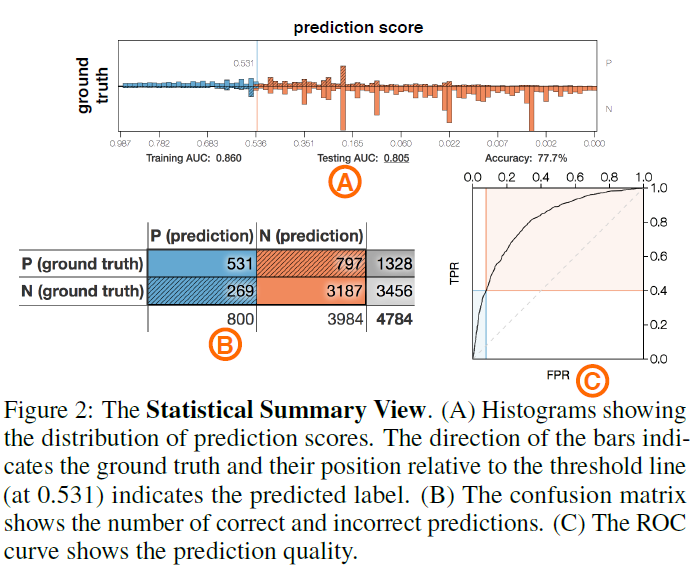
\includegraphics[scale=0.45]{pic/MA-Bilder/Literaturrecherche/25-statistsiche Summary.PNG}
    \caption{Statistische Zusammenfassung, entnommen aus \cite{krause2017workflow}}
    \label{Fig:Krause-statistischeSummary}
\end{wrapfigure}
Ein Beispiel für ein solches Tool wird an dieser Stelle kurz illustriert, um dessen Vorteile sichtbar zu machen. Der von \textcite{krause2017workflow}  entwickelte Workflow richtet sich an Domänen-Experten und Data Scientists. In ihrer Veröffentlichung wird demonstriert, wie sich durch Visualisierung ein Klassifikationsalgorithmus erklären lässt. Hierbei wird sich darauf konzentriert einzelne Instanzen zu erklären. Elemente ihrer Visualisierung sind: 
\begin{itemize}
    \item Aggregierte Statistiken verdeutlichen z.B. den Anteil korrekt und fehlerhaft klassifizierter Instanzen (vgl. Abbildung \ref{Fig:Krause-statistischeSummary})
    \item Erklärungen, welche die Relevanz einzelner Merkmale verdeutlichen
    \item Präsentation von Rohdaten, damit Nutzer diese als ergänzende Erklärungen heranziehen können
\end{itemize}
Das Prinzip des Workflows beruht auf Interaktivität, da dies die Bildung eines mentalen Modells auf Nutzerseite unterstützt und hiermit Algorithmusentscheidungen leichter nachzuvollziehen sind. Weiter abstrahieren sie von der Funktionsweise des ML-Algorithmus. Dies begründen sie darin, dass Nutzer, welche sich hiermit nicht auskennen, nur mit zu viel Wissen überfordert werden würden.
Workflow: - vorher: Erklärungen und Visualisierung (interaktiv Erklärungen für Daten anzeigen) - Outcome-Level: grundsätzliche Accuracy z.B. mit Confusion matrix - Feature-Level: Alle Erklärungen mit gleichen Merkmalen gebündelt anzeigen - Instance-Level: Erklärung für eine Instanz der Daten  Interaktive Auswahl an Erklärungen, Nutzer hat kein Zugriff auf die interen Struktur
Angewendete XAI-Methoden: Prospector [17], LIME, Martens und Provost [24 (Erklärungen für binären Input)
Grenzen des Ansatzes: nur binary-Data und kein Multihttps://de.overleaf.com/project/625d7985bac938c0561d8eda-Class
So sieht der Bums aus:
Statistische Zusammenfassung:

Explanation Explorer
\begin{figure}
    \centering
    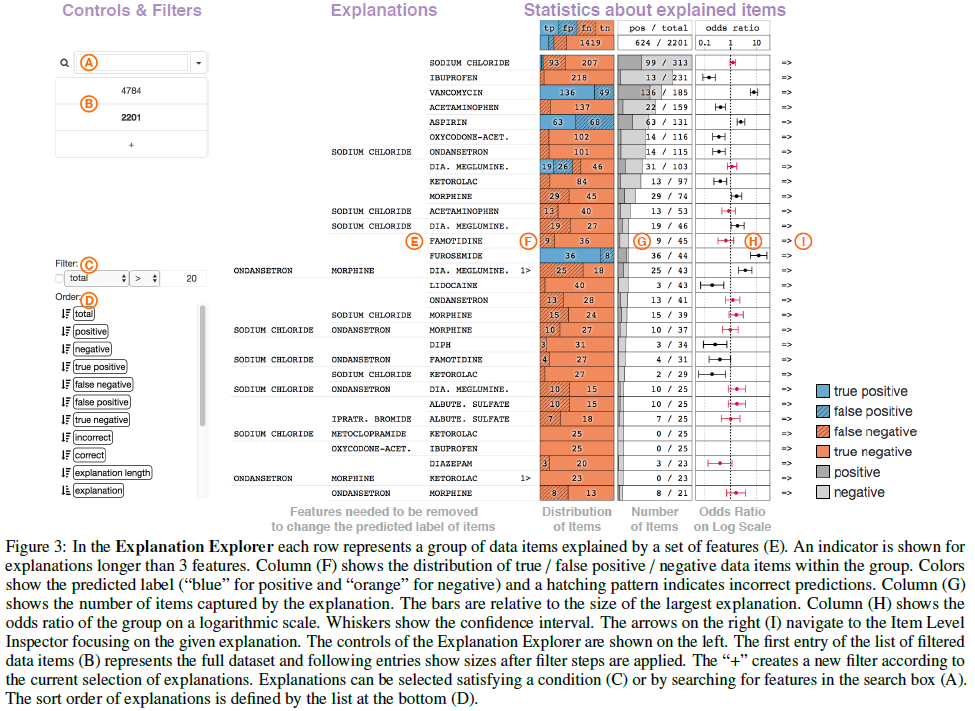
\includegraphics[scale=0.45]{pic/MA-Bilder/Literaturrecherche/25-explanationexplorer.PNG}
    \caption{explanation explorer, entommen aus: \cite{krause2017workflow}}
    \label{Fig:Krause-explanationExplorer}
\end{figure}
Itemlevel Explorer
\begin{figure}
    \centering
    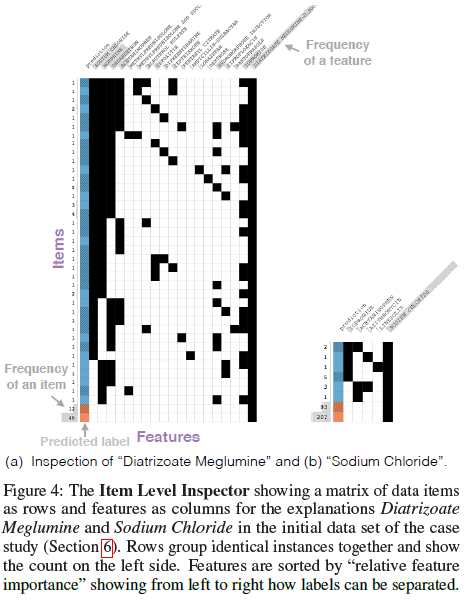
\includegraphics[scale=0.45]{pic/MA-Bilder/Literaturrecherche/25-itemlevelExplorer.PNG}
    \caption{item level explorer, entommen aus: \cite{krause2017workflow}}
    \label{Fig:Krause-itemLevelExplorer}
\end{figure}

Andere ähnliche Methoden wie die von \cite{krause2017workflow}: 
-ModelTracker [3]: Schnittstelle für Fehlererkennung und Fehlersuche bei binären Klassifizierern, die itemweise Verteilungen von Vorhersageergebnissen anzeigt. 
- Bilal et al.: confusion wheel visualization [1], um die Wahrscheinlichkeiten der Zugehörigkeit von Elementen zu verschiedenen Klassen für Mehrklassenklassifikatoren anzuzeigen. 
- Squares [26] bietet eine einzige, einheitliche Visualisierung von Leistungsmetriken und einen einfachen Zugang zu den Daten für das Debugging von Mehrklassenklassifikatoren.
- Cortez und Embrechts [9]: Ansatz der Sensitivitätsanalyse, der es den Benutzern ermöglicht, die Auswirkungen der Variation von Eingabewerten auf die Modellergebnisse zu verstehen
\subsection{XAI-Plattformen}
\todo[inline]{Ich überlege noch wie/ob ich einen Unterschied zwischen Visualisierungstools, Plattformen, Toolkits mache}
Zur Unterstützung bei der Anwendung von XAI-Methoden können Plattformen genutzt werden.

Für das Entwickeln von Plattformen haben \cite{rajabiyazdi2020machine} einige Charakteristiken identifiziert, welche optimalerweise vorhanden sein müssen. Zunächst wird auf die \emph{Mensch-Maschinen-Interaktion} eingegangen. In einer Benutzeroberfläche sollten kontextbezogene Informationen neben Gründen für eine Vorhersage vorhanden sein. Daneben sollte auch eine Darstellung über den Entwicklungsprozess vorhanden sein. \emph{Entscheidungsfindung} sollte durch eine Plattform auch unterstützt werden. Bei Entscheidungsunterstützungen sollte auch in der Plattform beachtet werden, dass diese den Plänen der Organisation folgen sollten. Daneben sollte der Prozess Entscheidungsfindung auch das Fachwissen der Nutzer unterstützen. Das Tool sollte außerdem Risiken aufzeigen, welcher mit einer Entscheidung, die auf Grundlage des Outputs getroffen werden einhergehen. Die \emph{Architektur} eines Systems ist im Idealfall in einer Plattform zu zeigen. Inhalte, die in Bezug auf die Architektur erfasst werden sollten sind z.B. die Datenerfassung, die Datenanalyse, oder das Bewerten von Prognosen. Auch Informationen anderer Systeme sollten integriert werden. Kommt es zu Ausfällen bei Prognosen, hat die Plattform auf diese aufmerksam zu machen. \cite{rajabiyazdi2020machine} haben selbst eine experimentelle Plattform vorgestellt, welche als Automated Reliability Decision Aid System (ARDAS) bezeichnet wird.

Zum Anwenden verschiedener XAI-Methoden existieren Software-Toolkits. Ein Beispiel ist das AI Explainability 360 Toolkit von IBM \footnote{https://aix360.mybluemix.net/} \cite{arya2021ai}. Dieses Toolkit unterstützt die Entwicklung von ML-Algorithmen in der Programmiersprache Python mithilfe von acht verschiedenen Erklärungsmethoden:
\begin{itemize}
    \item \emph{Boolean Decision Rules via Column Generation} werden mithilfe des BRCGExplainer erklärt, welcher binäre Klassifikation unterstützt und direkt interpretierbar ist \cite{dash2018boolean}
    \item Die direkt interpretierbaren \emph{Generalized Linear Rule Models} werden mithilfe des GLRMExplainer erklärt \cite{wei2019generalized}
    \item Der \emph{ProtodashExplainer} ist für das Erläutern von Datensätzen zuständig. Hier werden repräsentative Teile der Daten ausgewählt oder Testinstanzen erklärt \cite{gurumoorthy2019efficient}.
    \item Der \emph{ProfWeightExplainer} liefert globale Erklärungen durch das Darstellen von Gewichten neuronaler Netze \cite{dhurandhar2018improving}.
    \item Personenspezifische Erklärungen werden mithilfe des \emph{TEDExplainers} umgesetzt \cite{hind2019ted}.
    \item Die Methode von \cite{dhurandhar2018explanations} (\emph{CEMExplainer}) wird genutzt, um lokale Erklärungen zu generieren. Dies sind konstrative Erklärungen. Z.B. wird die Frage beantwortet, was minimal ausreichend ist, um die ursprüngliche Klassenvorhersage beizubehalten.
    \item Für Erklärungen von Bildern wird der \emph{CEMMAFImageExplainer} nach \cite{luss2019generating} eingesetzt.
    \item Abhängigkeiten von Merkmalen werden mithilfe von dem \emph{IPVAEExplainer} nach \cite{kumar2017variational} verdeutlicht.
\end{itemize}
Daneben bietet das Explainability 360 Toolkit auch Bewertungsmetriken an und eine erweiterbare Softwarearchitektur. \cite{arya2021ai} empfehlen für das Arbeiten mit ihrem Toolkit des Weiteren einen drei-schrittigen Ablauf, welcher zunächst das Filtern auf verschiedene Instanzen vorsieht. Daraufhin sollten Merkmale einzelner Instanzen präsentiert werden und diese sollten mit anderen Instanzen verglichen werden. Abschließend sollten Ekrlärungen generiert werden, z.B. kontrafaktische Erklärungen. Auch \cite{arya2021ai} weisen darauf hin, dass es schwierig ist zu entscheiden, welche Erklärung genau zu wählen ist. Zielgruppe dieses Tookits sind Entwickler und Data Scientists. Zur Unterstützung werden außerdem Tutorials angeboten, welche auch mit fachlichem Kontext (Medizin) vorhanden sind.
\begin{figure}[h]
    \centering
    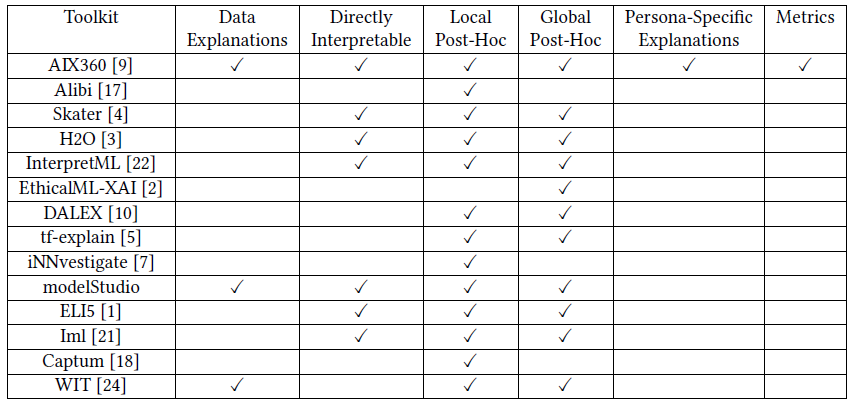
\includegraphics[scale=0.6]{pic/MA-Bilder/Literaturrecherche/30-Toolkits.PNG}
    \caption{Toolkits im Vergleich, entommen aus: \cite{arya2021ai}}
    \label{Fig:toolkitsvergleich}
\end{figure}

Neben dem Explainability 360 Toolkit weisen \cite{arya2021ai} auch auf andere Toolkits hin und vergleichen diese in Abbildung \ref{Fig:toolkitsvergleich} in Bezug auf ihre Funktionalitäten.
\subsection{Vorgehen bei Entwicklung}
\subsubsection{Vorgehensmodell für transparentes ML}
Grundsätzlich ist es bei einem praktischen Problem der realen Welt empfohlen, dass bei der Entwicklung von Software mit Endnutzern und Domänenexperten zusammengearbeitet wird und der gemeinsame Prozess so gestaltet wird, dass Endnutzer und Domänenexperten Feedback geben können \cite{zhou20182d}. Hierfür haben \cite{zhou20182d} ein Modell entwickelt, welches \emph{twodimensional (2D) transparency space} heißt und in Abbildung \ref{Fig:2D-Transparenz} zu sehen ist. Dieses Modell beschreibt den Workflow des transparenten ML (vgl. Kapitel \ref{subsubsec_TML}) und integriert sowohl ML-Experten als auch Domänennutzer in den Entwicklungsprozess.
\begin{figure}[h]
    \centering
    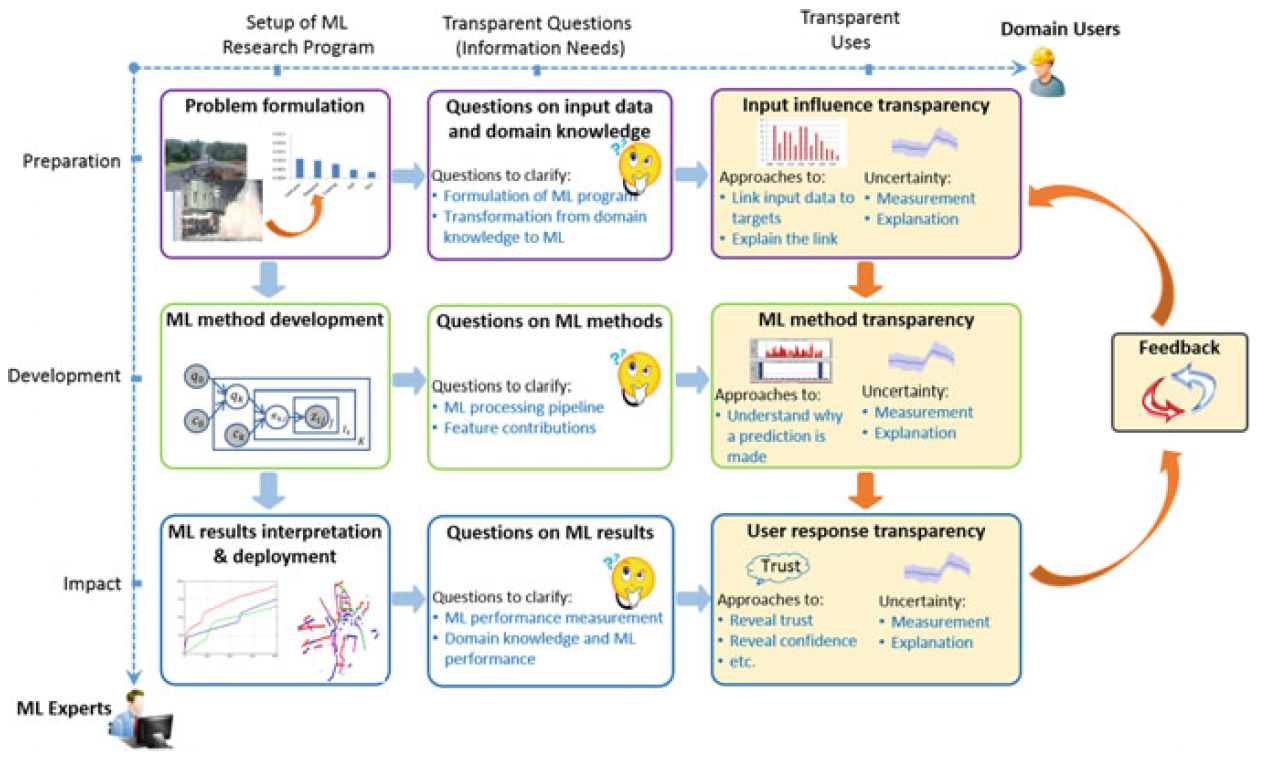
\includegraphics[scale=0.55]{pic/MA-Bilder/Literaturrecherche/4-2D-TransparencyWorkflow.PNG}
    \caption{2D transparency space, entnommen aus \cite{zhou20182d}}
    \label{Fig:2D-Transparenz}
\end{figure}

Aus Nutzerperspektive ergeben sich nach diesem Vorgehen drei Hauptaspekte. Zunächst wird das ML-Forschungsprogramm eingerichtet, was der Problemdefinition dient \cite{zhou20182d}. Gleichzeitig sollten Nutzer sogenannte \emph{transparente Fragen} stellen. Hier werden Informationsbedarfe für das ML-System aufgedeckt und beantwortet. Während der Vorbereitung ist beispielsweise wichtig, wie das Problem in ML überführt wird. In der Entwicklungsphase hingegen kann interessant sein, wie auf Daten zugegriffen wird. Wie die Leistung oder die Interpretation der Ergebnisse aussieht, sind transparente Fragen, welche während des Deployments stattfinden. Der dritte Baustein aus Nutzerperspektive ist der \emph{transparente Nutzen}. Während der Vorbereitung sollte verständlich gemacht werden, in welcher Form sich Inputs auf Outputs auswirken. Gleichzeitig sollen Unklarheiten über die Geschäftsanforderungen an das ML-System aufgelöst werden. Weiter sollte die ML-Methode selbst transparent gemacht werden, indem dessen Funktionsweise dargelegt wird. Eine Frage, welche hier beantwortet werden sollte ist z.B. \enquote{Warum wird diese mithilfe von Wissen über die Domäne Entscheidung getroffen?}. Während des Deployments sollten Reaktionen der Benutzer untersucht werden, um deren Vertrauen und Zuversicht zum ML-System zu stärken \cite{zhou20182d}. Ein wichtiger Bestandteil sind die Feedback-Schleifen. Sollte zum Ende des Projektes herausgefunden werden, dass Nutzer kein Vertrauen in das System haben, sollte die Problemdefinition und die Art der Überführung des Domänenproblems in ein ML-System erneut überdacht werden \cite{zhou20182d}.

Auch \cite{vaughan2020human} weist darauf hin, wie wichtig es ist verschiedene Stakeholder einzubeziehen, um dessen Bedürfnisse zu kennen. Dies sei besonders wichtig, um den Einsatz des ML-Systems im realen Kontext einschätzen zu können. Mögliche Stakeholder sind: Entwickler, Designer, Data Scientists, Manager, Regulierungsbehörden, Nutzer, Personen, welche in sonstiger Weise vom System betroffen sind.

Stakeholder früh einzubinden kann weiter das Problem des kognitiven Bias' bei Nutzern lösen, welcher bewirkt dass sie Erklärungen falsch oder anders verstehen. Erklärungen sollten Nutzern früh präsentiert werden, auch wenn dies bedeutet, dass noch Fehler in den Erklärungen vorhanden sein könnten\cite{nourani2021anchoring}. Für das Präsentieren der Erklärungen empfehlen \cite{nourani2021anchoring} zu Beginn high-level-Erklärungen, um ein grundsätzliches Bild darüber zu schaffen, wie das System funktioniert. Danach sollten einzelne Instanzen gezeigt werden. Die Erklärmethode sollte hier bewusst gewählt werden.

%\cite{hoang2021aid} haben AID: Active Distillation Machine to Leverage Pre-Trained Black-Box Models in Private Data Settings: aus bestehenden System Transparenz über Vorhersagen gewinnen, ohne auf alle Daten zugreifen zu dürfen --> Sicherstellung von Privacy. Dies wird durch die folgenden Module ermöglicht. Ausgehend von einem Blackbox-Modell, das auf privaten EHR -Daten trainiert wurde, lernt AID (I) ein Surrogatmodell, das globale und lokale interpretierbare Repräsentationen enthält; und (II) wendet eine aktive Strategie an, um das Blackbox-Modell sequentiell nach markierten Daten abzufragen, um sein Wissen in diese Repräsentationen zu destillieren.

%\cite{hernandez2021explainable} EU Proposal for Artificial Intelligence Act, 2021 sagt hochrisikosysteme (z.B. Luftfahrt, was Thema des Papers ist) sollen folgendes erfüllen: 1. Verwendung hochwertiger Trainings-, Validierungs- und Testdaten 2. Verwendung von Dokumentations- und Entwurfsprotokollierungsfunktionen, die eine kontinuierliche Dokumentation gewährleisten 3. Gewährleistung von Transparenz und Information der Nutzer über die Anwendung von KI-Systemen 4. Sicherstellung der menschlichen Aufsicht während des gesamten Prozesses 5. Sicherstellung der Genauigkeit, Robustheit und Cybersicherheit des Systems

\subsubsection{Transparenz während der Implementation}
Auch während der Implementation gibt es Maßnahmen, welche das ML-System transparenter machen. So empfiehlt z.B. \cite{huvc2021anomaly} das Anwenden einfacher Methoden.
Unterstützt werden kann transparente Entwicklung durch eine Toolbox namens Bob \footnote{https://www.idiap.ch/software/bob/}. Diese Toolbox bietet (Python-/C++)-Entwicklern Hilfestellungen bei der Siganlverarbeitung und dem ML. Unterstützt wird Reproduzierbarkeit durch Protokolle, aber auch durchschaubarer Code, Dokumentationen und Unit-Tests. 

Den Ansatz der Vereinfachung verfolgen auch \cite{zucker2020arbiter}, die eine eigene domänenspezifischen Sprache entwickelt haben, welche im Rahmen des ethischen ML neben Fairness, Zurechenbarkeit und Reproduzierbarkeit auch Transparenz gewährleistet. Unter einer domänenspezifischen Sprache, werden Programmiersprachen verstanden, welche nur in einem bestimmten Kontext eingesetzt werden. Hierdurch sind sie jedoch auch etwas begrenzter in ihrer Funktionalität. Diese domänenspezifische Sprache heißt \emph{Arbiter} und ist außerdem deklarativ. Dies bedeutet, dass Nutzer angeben, welches Ziel zu erreichen ist und das System selbst bestimmen kann, wie dies zu erreichen ist \cite{van2004concepts}. Transparenz während der Entwicklung wird mithilfe von \emph{Arbiter} vor allem dadurch geschaffen, dass Python Code kürzer dargestellt wird. Außerdem wird klarer herausgestellt, was eine bestimmte Zeile Code tut. Ein Beispiel für die Nutzung von \emph{Arbiter} ist in Abbildung \ref{Fig:Arbiter} zu sehen.
\begin{figure}
    \centering
    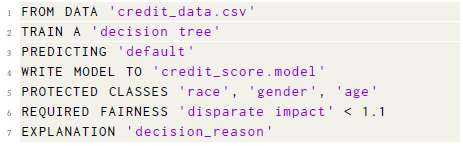
\includegraphics[scale=0.8]{pic/MA-Bilder/Literaturrecherche/45-CodeSnippet.PNG}
    \caption{Beispiel Arbiter, entnommen aus \cite{zucker2020arbiter}}
    \label{Fig:Arbiter}
\end{figure}

\subsubsection{AutoML}
Bei der Entwicklung eines ML-Systems kann es vorkommen, dass unterschiedliche Algorithmen ausprobiert werden. Zur automatisierten Unterstützung kann hierfür AutoML Anwendung finden. Dies sind Methoden, welche die Algorithmenauswahl und die Abstimmung der Parameter übernehmen, da es für Menschen zu aufwendig sein kann, dies händisch für eine Vielzahl an Möglichkeiten durchzuprobieren \cite{wang2019atmseer}. Um diesen automatischen Prozess transparent zu machen haben \cite{wang2019atmseer} das Tool \emph{ATMSeer} entwickelt. Dies ist ein Visualisierungstool, welches es Entwicklern ermöglicht einen Überblick über den AutoML-Prozess zu bekommen oder Statistiken auf unterschiedlichen Granularitätsebenen anzeigen zu lassen. 
%AuotML auch empfohlen von: \cite{waring2020automated}

\subsubsection{Verteiltes Lernen}
\begin{figure}[h]
    \centering
    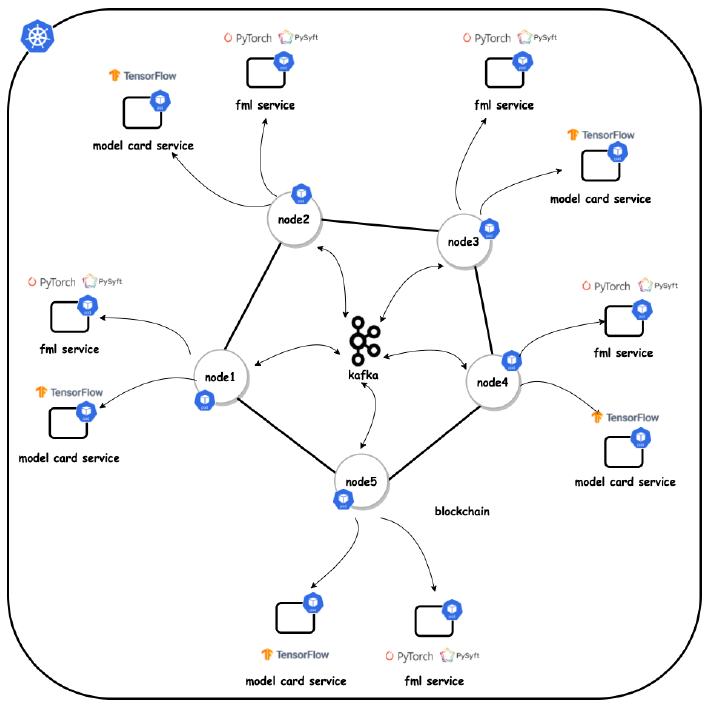
\includegraphics[scale=0.45]{pic/MA-Bilder/Literaturrecherche/56-BassaMLArchitektur.PNG}
    \caption{Architektur von Bassa-ML, entnommen aus: \cite{bandara2022bassa}}
    \label{Fig:Bass-ML-Architektur}
\end{figure}
Eine weitere Besonderheit bei dem Trainieren von ML-Modellen während der Entwicklung ist das verteilte Lernen. Dies sollte ursprünglich Datenschutzprobleme lösen, jedoch arbeiten die meisten Ansätze in der Praxis mit zentralisierten Koordination, welche anfällig für Angriffe von außen sind. Weiter besteht ein Problem beim verteilten Lernen darin, dass nicht klar ist, woher welche Daten stammen \cite{bandara2022bassa}.
\cite{bandara2022bassa} haben eine transparenzschaffende Maßnahme mithilfe der Blockchain-Technologie implementiert, welche Vertrauen und Transaprenz über die im verteilten Lernen erstellten Modelle schaffen soll. Ihre Lösung heißt Bassa-ML, welche ModelCards in einer Blockchain speichert und die Historie der verschiedenen Modelle transparent macht. Jeder Teilnehmer des Netzwerkes erstellt lokale Modelle und die zugehörigen ModelCards, welche zu lokalen Modellen aggregiert werden können, wenn Blöcke für das Block-Chain-Netzwerk erstellt werden. Die grobe Systemarchitektur ist schematisch in Abbildung \ref{Fig:Bass-ML-Architektur} dargestellt.

Auch \cite{zerka2020blockchain} machen sich die Vorteile von Block-Chain-Ansätzen zu nutze. Sie entwickelten \emph{Chained Distributed Machine learning (C-DistriM)}. Vorteile von solchen Ansätzen bestehen vor allem in der Transparenz über die Herkunft der Daten und in der Überwachung des Lernprozesses \cite{zerka2020blockchain}.
\subsection{Dokumentation}
\subsubsection{Dokumentation des ML-Algorithmus}
Für die Dokumentation des Algorithmus kann sich an Model Cards for Model Reporting orientiert werden.
\todo[inline]{Hier erkläre ich noch Model Cards for Model Reporting}
Es existieren auch Beispiele für die Anwendung von Model Cards for Model Reporting in der medizinischen Branche \cite{sendak2020human} sowie der Biologie \cite{grasso2020applying}.

Daneben können zur Dokumentation des Algorithmus auch Grafiken genutzt werden, welche häufig schon während der Entwicklung angewendet werden. So könnte eine Confusion-Matrix \cite{hasib2022machine} genau so wie die Darstellung von Precision, Recall, Specificity und F1-Score \cite{huvc2021anomaly} mit in die Dokumentation einfließen.
\todo[inline]{Hier werde ich noch kurz erklären, was die Metriken aussagen und vlt. Bilder einbauen}

\subsubsection{Dokumentation der Modellauswahl}
Auch die Modellauswahl sollte dokumentiert werden. So kann von Interesse sein, welche Verfahren ausprobiert wurden. Weiter könnte dokumentiert werden, ob oder wann z.B. um Überanpassung zu vermeiden mit dem Training gestoppt wurde \cite{de2018algorithmic}.

\subsubsection{Ganzheitliche Dokumentation}
Ein bekanntes Beispiel für die ganzheitliche Dokumentation eines ML-Systems ist ABOUT ML. Dies ist eine Sammlung von Best Pratices zur Dokumentation von Daten, Modellen und betrachtet hierbei den gesamten Lebenszyklus \cite{vaughan2020human, raji2019ml}. Daneben werden auch Artefakte oder Prozesse dokumentiert und es richtet sich an unterschiedliche Arten von Stakeholdern \cite{raji2019ml}.

Ein Framework, an dem sich bei der Dokumentation orientiert werden kann, wurde von \cite{hernandez2021explainable} im Bereich der Luftfahrt entwickelt. Dieses sollte zwar ursprünglich  setzt zwar den initialen Fokus darauf Vertrauen zu schaffen, aber kann auch zu mehr Transparenz beitragen. Aspekte, welche in die Dokumentation mit einfließen könnten, sind:
\begin{itemize}
    \item Zweck des Systems: Was macht der Algorithmus? Welcher Algorithmus wurde aus welchen Gründen ausgewählt (mögliche Gründe: Performance oder Genauigkeit)?
    \item Technische Robustheit: Datenquellen (Qualität, Zugang, Integrität, Schutz und Sicherheit), Lebenszyklus, Zuverlässigkeit, Reproduzierbarkeit, Interpretierbarkeit/Erklärbarkeit
    \item Maßnahmen im Bereich der IT-Sicherheit
    \item Darstellung von nutzerfreundlichen Erklärungen sowie Reporting und Auditing
\end{itemize}

Ein weiteres Framework wurde von \cite{garbin2022assessing} entwickelt. Dieses legt zwar auch den Fokus eher auf Audits von ML-Systemen, kann jedoch auch dabei helfen ein System transparenter zu machen. In folgender Aufzählung sind kurz die wichtigsten Aspekte dargestellt, gekürzt um die Punkte, welche sich konkret auf das Durchführen von Audits beziehen:
\todo[inline]{Die beiden Checklisten gieße ich eventuell noch in den Text - auf jeden Fall fließen die Inhalte irgendwie in meine Handreichung ein, da besonders die zweite Abbildung meine dritte Forschungsfrage beantwortet}
\begin{itemize}
    \item Scoping: Dokumentation der Systemanforderungen und der angewendeten ML-Prinzipen, Use-Cases für ein ethisches Review und einer social impact analysis
    \item Mapping: Mapping von Stakeholdern auf Anforderungen, Dokumentation der Stakeholder-Interviews
    \item Artefakte: Checklisten, Model Cards, Datasheets for Datesets
    \item Testen: gegenseitige Prüfung der Dokumentation
    \item Reflektion: Zeitplan
\end{itemize}
Zusätzlich geben \cite{garbin2022assessing} einen Überblick über mögliche Checklisten und geben an, welche Checkliste in welchem zeitlichen Stadium der ML-Entwicklung \ref{Fig:ChecklisteJeStadium} angewendet wird und an wen diese sich richtet \ref{Fig:ChecklisteJeRolle}.
\begin{figure}[h]
    \centering
    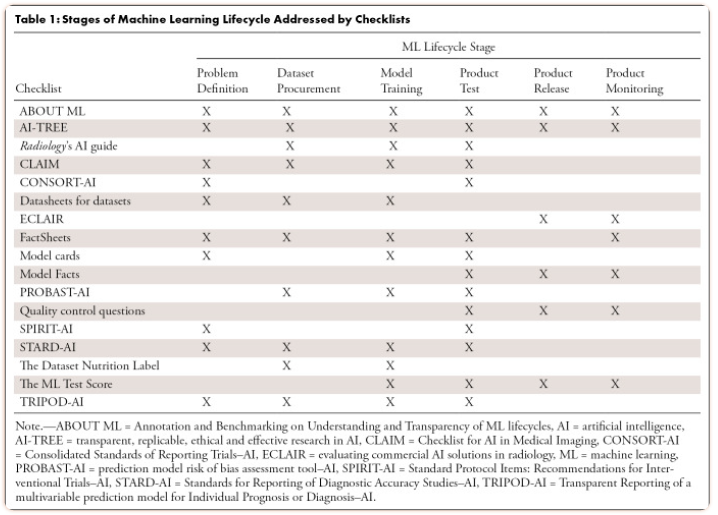
\includegraphics[scale=0.45]{pic/MA-Bilder/Literaturrecherche/49-ChecklistNachStages.PNG}
    \caption{Checkliste je ML-Stadium, entommen aus: \cite{garbin2022assessing}}
    \label{Fig:ChecklisteJeStadium}
\end{figure}
\begin{figure}[h]
    \centering
    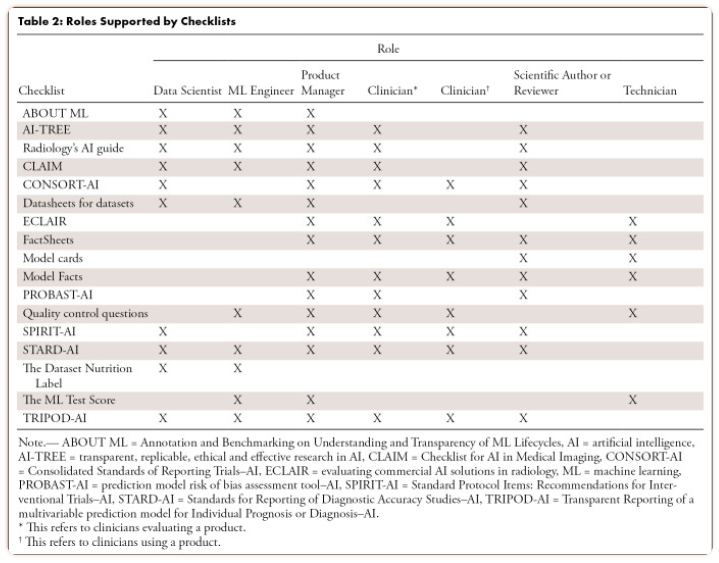
\includegraphics[scale=0.45]{pic/MA-Bilder/Literaturrecherche/49-ChecklistNachRollen.PNG}
    \caption{Checkliste je Publikum, entommen aus: \cite{garbin2022assessing}}
    \label{Fig:ChecklisteJeRolle}
\end{figure}

Weiterführend finden sich in der Veröffentlichung von \cite{garbin2022assessing} Hinweise darüber, wann welche Dokumentationsmethode eingesetzt werden kann. Konkret gehen sie auf Datasheets for Datasets, Modelcards und Modelfact ein (siehe Abbildung \ref{Fig:Datsheet_Datest_Modelfact}).
\begin{figure}
    \centering
    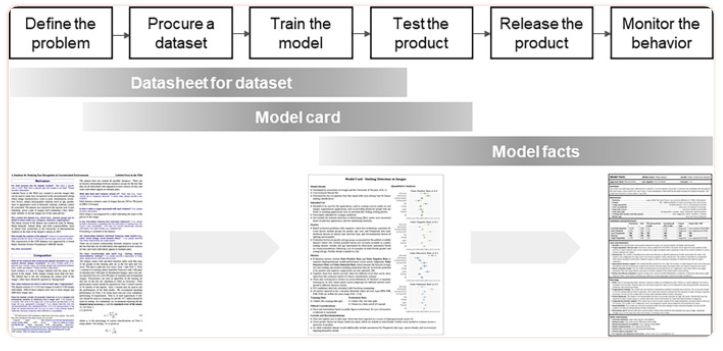
\includegraphics[scale=0.45]{pic/MA-Bilder/Literaturrecherche/49-ZusammenspielDatasheets_Modelcard_Modelfacts.PNG}
    \caption{Übersicht XAI-Methode mit Audience, entommen aus: \cite{garbin2022assessing}}
    \label{Fig:Datsheet_Datest_Modelfact}
\end{figure}
\subsection{Probleme mit Transparenz}
Bisher wurden in der Arbeit neben transparenzschaffenden Maßnahmen vor allem die positiven Aspekte von Transparenz im ML herausgestellt. Jedoch ergab die Literaturrecherche auch einige negative Aspekte von Transparenz oder deckte Bereiche auf, in denen noch Forschungs- oder Klärungsbedarf besteht.

\subsubsection{Offene Fragen bei Transparenz} 
\cite{zhou20182d} beschreiben das Konzept des transparenten ML (vgl. Kapitel \ref{subsec_Konzepte}) und führen hierbei zusätzlich offene Fragen an, die von ihrem Konzept noch nicht abgedeckt werden. So beschreiben sie, dass grundsätzlich Vertrauen bei transparenten ML zwar wichtig ist, jedoch wenig darüber bekannt ist, wie Vertrauen in Menschen entsteht. \cite{vaughan2020human} führen hierzu an, dass es vorkomme, dass Menschen einem ML-System mehr vertrauen, welches viele Features benutzt, obwohl sie es nicht verstehen. Ein Modell, welches sie verstehen, aber beispielsweise nur wenige Features nutze, führt zu weniger Vertrauen in das System.
Weiter bewege nach \cite{zhou20182d} Nutzer von ML-Systemen das Risiko bei der Nutzung eines solchen Systems. So seien diese Systeme nicht perfekt und ideal wäre eine Abwägung der Kosten, wenn auf Grundlage eines Systems in der realen Welt eine falsche Entscheidung getroffen wird. Weiter leiden bisherige XAI-Methoden vor allem unter einer Verallgemeinerung der Erklärungsempfänger. So bringen alle menschlichen Betrachter unterschiedliche Bildung, Kultur oder Geschlecht mit, was die Anforderungen an die Art und Weise der geforderten Kommunikation bedingt.
Besonders zu viel Transparenz und die Kommunikation besonders komplizierter Modelle sei nicht geeignet für Fachfremde, da hier das technische Hintergrundwissen nicht vorhanden ist \cite{de2018algorithmic}. Des Weiteren ist schwer zu entscheiden, welches Maß an Transparenz gut ist. Zu wenig Transparenz kann problematisch werden \cite{kulesza2013too} und wichtige Aspekte werden einfach ausgelassen \cite{blacklaws2018algorithms}. Zu viel Transparenz und zu viele Erklärungen führen jedoch dazu, dass Nutzer sehr viel Zeit und unter Umständen Wissensakkumulation dafür aufbringen müssen, die Erklärungen zu verstehen \cite{blacklaws2018algorithms}. \cite{blacklaws2018algorithms} sprechen hier von dem Transparenzparadoxon.
Auch \cite{biessmann2021turing} fanden heraus, dass das Erstellen von \enquote{guten und nutzerfreundlichen} Erklärungen nicht trivial ist. Sie führten einen Touringtest durch, in denen die Studienteilnehmer bestimmen sollten, ob eine vorliegende Erklärung (Markierung von 3 Buzz-Words bei einer Textklassifikation) von einem Menschen oder einer angewendeten XAI-Methode getroffen wurde. Ergebnis der Studie war, dass Menschen später nicht in der Lage waren, zu sagen, ob eine Klassifikationsentscheidung automatisiert oder von Hand getroffen wurde.

\subsubsection{Zeitaufwand}
Des Weiteren ist es laut \cite{vaughan2020human} vorgekommen, dass Nutzer das Erstellen eines mentalen Modells mithilfe von Erklärungen als Zeitverschwendung betrachteten. 

\subsubsection{Gefahren durch Transparenz}
Neben den bereits angeführten Problemen können einige Aspekte von Transparenz jedoch auch schwerwiegende Folgen in der Praxis haben, wenn Systeme z.B. in der Medizin oder im Verkehr eingesetzt werden. 
Erklärungen lassen sich z.B. manipulieren, sodass Nutzer den Erklärungen nicht mehr trauen können \cite{tjoa2020survey}. Ein Beispiel hierzu wird von \cite{ghorbani2019interpretation} beschrieben, das zeigt, wie aus einem originalen Bild ein für den Nutzer kaum zu unterscheidbares zweites Bild erstellt werden kann, dass jedoch eine gänzlich andere Erklärung erhält.
Neben funktionalen Problemen, welche kritisch für das Vertrauen und die korrekte Anwendung sind, bestehen noch weitere Probleme in Bezug auf Datenschutz \cite{de2018algorithmic}. Dies liegt auf der Hand, wenn wie in \todo[inline]{Hier verweise ich noch auf die Stelle (die habe ich nur noch nicht geschrieben :D)} beschrieben konkrete Beispiele oder Auszüge aus den Trainingsdaten offen gelegt werden, jedoch existieren auch subtilere Angriffe auf die Privatsphäre bei ML-Systemen. \cite{shokri2017membership} beschreiben die \enquote{Membership Inference Attack}, welche sich bei ML-Algorithmen anwenden lässt und es einem Angreifer ermöglicht herauszufinden, ob ein bestimmter Datenpunkt in dem genutzten Trainingsdatensatz vorhanden war.

%Fairness-Methoden gibt es auch noch und es wurden auch welche gefunden, aber wegen Zeit wurde sich darauf nicht konzentriert (Quelle 5, 7, 18, 19, 22, 57, 59, 62, 63, denton2020bringing, 65 )
%Ausblick für später: \cite{de2018algorithmic} Kann Transparenz Accountability ersetzen?
%Ethische Betrachtung/Motivation für Transparenz: 46
%rechtliche Betrachtung: 54

%Branchenspezifische Quellen:
%-Medizin: \cite{garbin2022assessing} \cite{keller2020augmenting} \cite{zerka2020blockchain}
%- Luftfahrt: \cite{hernandez2021explainable}, \cite{westin2020building}
%- IT-Security \cite{wang2020explainable}, \cite{huvc2021anomaly}, \cite{pan2021automated}


%Stehen geblieben bei Zeile: 397
% ===========================Selbstständigkeitserklärung======================
\chapter*{Eidesstattliche Versicherung} % war: Selbständigkeitserklärung
\vspace{1cm}

\todo[noline]{Bitte verwenden Sie hier in jedem Fall die offizielle von der Prüfungsbehörde vorgegebene Formulierung der Selbständigkeitserklärung.}
%
Hiermit versichere ich an Eides statt, dass ich die vorliegende Arbeit selbstständig verfasst und keine anderen als die angegebenen Hilfsmittel – insbesondere keine im Quellenverzeichnis nicht benannten Internet-Quellen – benutzt habe. Alle Stellen, die wörtlich oder sinngemäß aus Veröffentlichungen entnommen wurden, sind als solche kenntlich gemacht. Ich versichere weiterhin, dass ich die Arbeit vorher nicht in einem anderen Prüfungsverfahren eingereicht habe und die eingereichte schriftliche Fassung der auf dem elektronischen Speichermedium entspricht.

Ggf. streichen: Ich bin damit einverstanden, dass meine Abschlussarbeit in den Bestand der Fachbereichsbibliothek eingestellt wird.

\makeatletter
Hamburg, den {\@date}
\makeatother

\vspace{2cm}
\rule{6cm}{0.25pt}\\
\makeatletter
{\@author} \par
\makeatother


% =============================Literaturverzeichnis=============================
\begin{raggedright}         % Schaltet Blocksatz ab, erzeugt ein stimmigeres
                            %  Schriftbild im Literaturverzeichnis.
  \printbibliography        % Falls Biblatex verwendet wird.
  \label{sec:literaturverzeichnis}
\end{raggedright}


% ===================================Anhang=====================================
\appendix
\setcounter{figure}{0}
\renewcommand\thetable{A.\arabic{figure}}
\setcounter{table}{0}
\renewcommand\thetable{A.\arabic{table}}


% ================================Todo list==============================
\listoftodos
 \todototoc

\end{document}